\documentclass[twoside]{book}

% Packages required by doxygen
\usepackage{calc}
\usepackage{doxygen}
\usepackage{graphicx}
\usepackage[utf8]{inputenc}
\usepackage{makeidx}
\usepackage{multicol}
\usepackage{multirow}
\usepackage{textcomp}
\usepackage[table]{xcolor}

% NLS support packages
\usepackage[french]{babel}

% Font selection
\usepackage[T1]{fontenc}
\usepackage{mathptmx}
\usepackage[scaled=.90]{helvet}
\usepackage{courier}
\usepackage{amssymb}
\usepackage{sectsty}
\renewcommand{\familydefault}{\sfdefault}
\allsectionsfont{%
  \fontseries{bc}\selectfont%
  \color{darkgray}%
}
\renewcommand{\DoxyLabelFont}{%
  \fontseries{bc}\selectfont%
  \color{darkgray}%
}

% Page & text layout
\usepackage{geometry}
\geometry{%
  a4paper,%
  top=2.5cm,%
  bottom=2.5cm,%
  left=2.5cm,%
  right=2.5cm%
}
\tolerance=750
\hfuzz=15pt
\hbadness=750
\setlength{\emergencystretch}{15pt}
\setlength{\parindent}{0cm}
\setlength{\parskip}{0.2cm}
\makeatletter
\renewcommand{\paragraph}{%
  \@startsection{paragraph}{4}{0ex}{-1.0ex}{1.0ex}{%
    \normalfont\normalsize\bfseries\SS@parafont%
  }%
}
\renewcommand{\subparagraph}{%
  \@startsection{subparagraph}{5}{0ex}{-1.0ex}{1.0ex}{%
    \normalfont\normalsize\bfseries\SS@subparafont%
  }%
}
\makeatother

% Headers & footers
\usepackage{fancyhdr}
\pagestyle{fancyplain}
\fancyhead[LE]{\fancyplain{}{\bfseries\thepage}}
\fancyhead[CE]{\fancyplain{}{}}
\fancyhead[RE]{\fancyplain{}{\bfseries\leftmark}}
\fancyhead[LO]{\fancyplain{}{\bfseries\rightmark}}
\fancyhead[CO]{\fancyplain{}{}}
\fancyhead[RO]{\fancyplain{}{\bfseries\thepage}}
\fancyfoot[LE]{\fancyplain{}{}}
\fancyfoot[CE]{\fancyplain{}{}}
\fancyfoot[RE]{\fancyplain{}{\bfseries\scriptsize Généré le Dimanche 25 Mai 2014 22\-:27\-:42 pour Simulation d'evacuation d'immeuble avec systeme multi-\/agents par Doxygen }}
\fancyfoot[LO]{\fancyplain{}{\bfseries\scriptsize Généré le Dimanche 25 Mai 2014 22\-:27\-:42 pour Simulation d'evacuation d'immeuble avec systeme multi-\/agents par Doxygen }}
\fancyfoot[CO]{\fancyplain{}{}}
\fancyfoot[RO]{\fancyplain{}{}}
\renewcommand{\footrulewidth}{0.4pt}
\renewcommand{\chaptermark}[1]{%
  \markboth{#1}{}%
}
\renewcommand{\sectionmark}[1]{%
  \markright{\thesection\ #1}%
}

% Indices & bibliography
\usepackage{natbib}
\usepackage[titles]{tocloft}
\setcounter{tocdepth}{3}
\setcounter{secnumdepth}{5}
\makeindex

% Custom commands
\newcommand{\clearemptydoublepage}{%
  \newpage{\pagestyle{empty}\cleardoublepage}%
}


%===== C O N T E N T S =====

\begin{document}

% Titlepage & ToC
\pagenumbering{roman}
\begin{titlepage}
\vspace*{7cm}
\begin{center}%
{\Large Simulation d'evacuation d'immeuble avec systeme multi-\/agents \\[1ex]\large 0.\-1 }\\
\vspace*{1cm}
{\large Généré par Doxygen 1.8.5}\\
\vspace*{0.5cm}
{\small Dimanche 25 Mai 2014 22:27:42}\\
\end{center}
\end{titlepage}
\clearemptydoublepage
\tableofcontents
\clearemptydoublepage
\pagenumbering{arabic}

%--- Begin generated contents ---
\chapter{Index hiérarchique}
\section{Hiérarchie des classes}
Cette liste d'héritage est classée approximativement par ordre alphabétique \-:\begin{DoxyCompactList}
\item \contentsline{section}{Agent\-Package}{\pageref{struct_agent_package}}{}
\item \contentsline{section}{Coordonnes2\-D}{\pageref{class_coordonnes2_d}}{}
\item \contentsline{section}{Couleur}{\pageref{class_couleur}}{}
\item \contentsline{section}{Fenetre}{\pageref{class_fenetre}}{}
\item \contentsline{section}{Graphe}{\pageref{class_graphe}}{}
\item \contentsline{section}{Node}{\pageref{class_node}}{}
\item Observer\begin{DoxyCompactList}
\item \contentsline{section}{T\-E\-R\-Observer}{\pageref{class_t_e_r_observer}}{}
\end{DoxyCompactList}
\item \contentsline{section}{Pathfinder}{\pageref{class_pathfinder}}{}
\item Turtle\begin{DoxyCompactList}
\item \contentsline{section}{Humain}{\pageref{class_humain}}{}
\item \contentsline{section}{Mur}{\pageref{class_mur}}{}
\end{DoxyCompactList}
\end{DoxyCompactList}

\chapter{Index des classes}
\section{Liste des classes}
Liste des classes, structures, unions et interfaces avec une brève description \-:\begin{DoxyCompactList}
\item\contentsline{section}{{\bf Agent\-Package} \\*Objet servant d'archive pour le transfert d'attribut des agents d'un processus à un autre }{\pageref{struct_agent_package}}{}
\item\contentsline{section}{{\bf Coordonnes2\-D} \\*Classe representant une position(coordonnees) d'un point }{\pageref{class_coordonnes2_d}}{}
\item\contentsline{section}{{\bf Couleur} \\*Classe representant une \doxyref{Couleur}{p.}{class_couleur} }{\pageref{class_couleur}}{}
\item\contentsline{section}{{\bf Fenetre} \\*Classe representant une \doxyref{Fenetre}{p.}{class_fenetre} S\-D\-L }{\pageref{class_fenetre}}{}
\item\contentsline{section}{{\bf Graphe} \\*Classe representant le monde Repast en memoire }{\pageref{class_graphe}}{}
\item\contentsline{section}{{\bf Humain} \\*Classe representant un agent humain }{\pageref{class_humain}}{}
\item\contentsline{section}{{\bf Mur} \\*Classe representant un \doxyref{Mur}{p.}{class_mur} }{\pageref{class_mur}}{}
\item\contentsline{section}{{\bf Node} \\*Classe representant un \doxyref{Node}{p.}{class_node} Un \doxyref{Node}{p.}{class_node} est une \char`\"{}case\char`\"{} de la matrice representant le monde Repast, chaque node contient les heuristiques,g,h et f, une position X et Y , un \doxyref{Node}{p.}{class_node} Parent, et un boolean indiquant si le node est un mur ou pas }{\pageref{class_node}}{}
\item\contentsline{section}{{\bf Pathfinder} \\*Classe representant une instance de l'algorithme A$\ast$ }{\pageref{class_pathfinder}}{}
\item\contentsline{section}{{\bf T\-E\-R\-Observer} \\*Classe representant un observateur, qui s'occupe de la gestion des agents dans ce processus }{\pageref{class_t_e_r_observer}}{}
\end{DoxyCompactList}

\chapter{Index des fichiers}
\section{Liste des fichiers}
Liste de tous les fichiers documentés avec une brève description \-:\begin{DoxyCompactList}
\item\contentsline{section}{code/include/{\bf Agent\-Package.\-h} \\*Classe representant une archive serialisee }{\pageref{_agent_package_8h}}{}
\item\contentsline{section}{code/include/{\bf coordonnes2d.\-h} \\*Classe representant une position(coordonnees) d'un point }{\pageref{coordonnes2d_8h}}{}
\item\contentsline{section}{code/include/{\bf couleur.\-h} \\*Classe representant une \doxyref{Couleur}{p.}{class_couleur} }{\pageref{couleur_8h}}{}
\item\contentsline{section}{code/include/{\bf fenetre.\-h} \\*Classe representant une fenetre S\-D\-L }{\pageref{fenetre_8h}}{}
\item\contentsline{section}{code/include/{\bf Graphe.\-h} \\*Classe representant le monde Repast en memoire afin d'appliquer l'algorithme A$\ast$ }{\pageref{_graphe_8h}}{}
\item\contentsline{section}{code/include/{\bf Humain.\-h} \\*Classe representant un agent \doxyref{Humain}{p.}{class_humain} }{\pageref{_humain_8h}}{}
\item\contentsline{section}{code/include/{\bf Mur.\-h} \\*Classe representant un \doxyref{Mur}{p.}{class_mur} }{\pageref{_mur_8h}}{}
\item\contentsline{section}{code/include/{\bf Node.\-h} \\*Classe representant un \doxyref{Node}{p.}{class_node} }{\pageref{_node_8h}}{}
\item\contentsline{section}{code/include/{\bf Path\-Finder.\-h} \\*Classe representant une instance de l'algorithme A$\ast$ }{\pageref{_path_finder_8h}}{}
\item\contentsline{section}{code/include/{\bf T\-E\-R\-Observer.\-h} \\*Classe representant un \doxyref{T\-E\-R\-Observer}{p.}{class_t_e_r_observer} }{\pageref{_t_e_r_observer_8h}}{}
\end{DoxyCompactList}

\chapter{Documentation des classes}
\section{Référence de la structure Agent\-Package}
\label{struct_agent_package}\index{Agent\-Package@{Agent\-Package}}


Objet servant d'archive pour le transfert d'attribut des agents d'un processus à un autre.  




{\ttfamily \#include $<$Agent\-Package.\-h$>$}

\subsection*{Fonctions membres publiques}
\begin{DoxyCompactItemize}
\item 
{\footnotesize template$<$class Archive $>$ }\\void {\bfseries serialize} (Archive \&ar, const unsigned int version)\label{struct_agent_package_a0ffe06e4b5a46a985ce640cd061f4324}

\item 
repast\-::\-Agent\-Id {\bfseries get\-Id} () const \label{struct_agent_package_a2a7beccac99040e280a4e79f84345179}

\end{DoxyCompactItemize}
\subsection*{Attributs publics}
\begin{DoxyCompactItemize}
\item 
int {\bf id}
\item 
int {\bf proc}
\item 
int {\bf type}
\item 
int {\bf current\-Proc}
\item 
std\-::vector$<$ int $>$ {\bf chemin\-X}
\item 
std\-::vector$<$ int $>$ {\bf chemin\-Y}
\item 
int {\bf etape}
\item 
int {\bf type\-Personne}
\end{DoxyCompactItemize}


\subsection{Description détaillée}
Objet servant d'archive pour le transfert d'attribut des agents d'un processus à un autre. 

\subsection{Documentation des données membres}
\index{Agent\-Package@{Agent\-Package}!chemin\-X@{chemin\-X}}
\index{chemin\-X@{chemin\-X}!AgentPackage@{Agent\-Package}}
\subsubsection[{chemin\-X}]{\setlength{\rightskip}{0pt plus 5cm}std\-::vector$<$int$>$ Agent\-Package\-::chemin\-X}\label{struct_agent_package_a7023c0492848b76c886feed44c97dbbe}
attribut chemin\-X de la classe \doxyref{Humain}{p.}{class_humain} \index{Agent\-Package@{Agent\-Package}!chemin\-Y@{chemin\-Y}}
\index{chemin\-Y@{chemin\-Y}!AgentPackage@{Agent\-Package}}
\subsubsection[{chemin\-Y}]{\setlength{\rightskip}{0pt plus 5cm}std\-::vector$<$int$>$ Agent\-Package\-::chemin\-Y}\label{struct_agent_package_aa4d44851a12b4a5cbb965999c9f325cd}
attribut chemin\-Y de la classe \doxyref{Humain}{p.}{class_humain} \index{Agent\-Package@{Agent\-Package}!current\-Proc@{current\-Proc}}
\index{current\-Proc@{current\-Proc}!AgentPackage@{Agent\-Package}}
\subsubsection[{current\-Proc}]{\setlength{\rightskip}{0pt plus 5cm}int Agent\-Package\-::current\-Proc}\label{struct_agent_package_acce31a89aa42cc20ea8e346dabf789d9}
id du processus courant \index{Agent\-Package@{Agent\-Package}!etape@{etape}}
\index{etape@{etape}!AgentPackage@{Agent\-Package}}
\subsubsection[{etape}]{\setlength{\rightskip}{0pt plus 5cm}int Agent\-Package\-::etape}\label{struct_agent_package_abf854b3cfca5add73170fdc862b8b477}
attribut etape de la classe \doxyref{Humain}{p.}{class_humain} \index{Agent\-Package@{Agent\-Package}!id@{id}}
\index{id@{id}!AgentPackage@{Agent\-Package}}
\subsubsection[{id}]{\setlength{\rightskip}{0pt plus 5cm}int Agent\-Package\-::id}\label{struct_agent_package_acb97295bf92e52e7791297ccfe00a9f0}
id de l'agent \index{Agent\-Package@{Agent\-Package}!proc@{proc}}
\index{proc@{proc}!AgentPackage@{Agent\-Package}}
\subsubsection[{proc}]{\setlength{\rightskip}{0pt plus 5cm}int Agent\-Package\-::proc}\label{struct_agent_package_a424b83e665a649a53251684d53b7f6ec}
id processus createur de l'agent \index{Agent\-Package@{Agent\-Package}!type@{type}}
\index{type@{type}!AgentPackage@{Agent\-Package}}
\subsubsection[{type}]{\setlength{\rightskip}{0pt plus 5cm}int Agent\-Package\-::type}\label{struct_agent_package_a47cb43c3eb16f7ab9fed25c310ea1f7a}
type d'agent \index{Agent\-Package@{Agent\-Package}!type\-Personne@{type\-Personne}}
\index{type\-Personne@{type\-Personne}!AgentPackage@{Agent\-Package}}
\subsubsection[{type\-Personne}]{\setlength{\rightskip}{0pt plus 5cm}int Agent\-Package\-::type\-Personne}\label{struct_agent_package_ac2a45d712ab4e8befb526865a12d67f3}
attribut type\-Personne de la classe \doxyref{Humain}{p.}{class_humain} 

La documentation de cette structure a été générée à partir du fichier suivant \-:\begin{DoxyCompactItemize}
\item 
code/include/{\bf Agent\-Package.\-h}\end{DoxyCompactItemize}

\section{Référence de la classe Coordonnes2\-D}
\label{class_coordonnes2_d}\index{Coordonnes2\-D@{Coordonnes2\-D}}


Classe representant une position(coordonnees) d'un point.  




{\ttfamily \#include $<$coordonnes2d.\-h$>$}

\subsection*{Fonctions membres publiques}
\begin{DoxyCompactItemize}
\item 
{\bf Coordonnes2\-D} ()
\begin{DoxyCompactList}\small\item\em Constructeur. \end{DoxyCompactList}\item 
{\bf Coordonnes2\-D} (int X, int Y)
\begin{DoxyCompactList}\small\item\em Constructeur. \end{DoxyCompactList}\item 
{\bf Coordonnes2\-D} (const {\bf Coordonnes2\-D} \&c)
\begin{DoxyCompactList}\small\item\em Constructeur. \end{DoxyCompactList}\item 
virtual {\bf $\sim$\-Coordonnes2\-D} ()
\begin{DoxyCompactList}\small\item\em Destructeur. \end{DoxyCompactList}\item 
int {\bf get\-X} () const 
\begin{DoxyCompactList}\small\item\em Getter. \end{DoxyCompactList}\item 
int {\bf get\-Y} () const 
\begin{DoxyCompactList}\small\item\em Getter. \end{DoxyCompactList}\item 
int {\bf get\-Cadran} () const 
\begin{DoxyCompactList}\small\item\em Getter. \end{DoxyCompactList}\item 
void {\bf set\-X} (int X)
\begin{DoxyCompactList}\small\item\em Setter. \end{DoxyCompactList}\item 
void {\bf set\-Y} (int Y)
\begin{DoxyCompactList}\small\item\em Setter. \end{DoxyCompactList}\item 
void {\bf set\-Cadran} (int val)
\begin{DoxyCompactList}\small\item\em Setter. \end{DoxyCompactList}\end{DoxyCompactItemize}
\subsection*{Attributs protégés}
\begin{DoxyCompactItemize}
\item 
int {\bf m\-\_\-\-X}
\item 
int {\bf m\-\_\-\-Y}
\item 
int {\bf m\-\_\-cadran}
\end{DoxyCompactItemize}


\subsection{Description détaillée}
Classe representant une position(coordonnees) d'un point. 

La classe est composee des coordonnees x et y d'un point ainsi que le cadran dans lequel il se trouve. 

\subsection{Documentation des constructeurs et destructeur}
\index{Coordonnes2\-D@{Coordonnes2\-D}!Coordonnes2\-D@{Coordonnes2\-D}}
\index{Coordonnes2\-D@{Coordonnes2\-D}!Coordonnes2D@{Coordonnes2\-D}}
\subsubsection[{Coordonnes2\-D}]{\setlength{\rightskip}{0pt plus 5cm}Coordonnes2\-D\-::\-Coordonnes2\-D (
\begin{DoxyParamCaption}
{}
\end{DoxyParamCaption}
)}\label{class_coordonnes2_d_aa5b01dbc1c5305dbf1dd51f20eeec05e}


Constructeur. 

Default constructor

Constructeur de la classe \doxyref{Coordonnes2\-D}{p.}{class_coordonnes2_d} \index{Coordonnes2\-D@{Coordonnes2\-D}!Coordonnes2\-D@{Coordonnes2\-D}}
\index{Coordonnes2\-D@{Coordonnes2\-D}!Coordonnes2D@{Coordonnes2\-D}}
\subsubsection[{Coordonnes2\-D}]{\setlength{\rightskip}{0pt plus 5cm}Coordonnes2\-D\-::\-Coordonnes2\-D (
\begin{DoxyParamCaption}
\item[{int}]{X, }
\item[{int}]{Y}
\end{DoxyParamCaption}
)}\label{class_coordonnes2_d_a3a4031367715512fb9d3aad9bc9a5564}


Constructeur. 

Constructeur de la classe \doxyref{Coordonnes2\-D}{p.}{class_coordonnes2_d}


\begin{DoxyParams}{Paramètres}
{\em X} & \-: coordonnee X a stocker \\
\hline
{\em Y} & \-: coordonnee Y a stocker \\
\hline
\end{DoxyParams}
\index{Coordonnes2\-D@{Coordonnes2\-D}!Coordonnes2\-D@{Coordonnes2\-D}}
\index{Coordonnes2\-D@{Coordonnes2\-D}!Coordonnes2D@{Coordonnes2\-D}}
\subsubsection[{Coordonnes2\-D}]{\setlength{\rightskip}{0pt plus 5cm}Coordonnes2\-D\-::\-Coordonnes2\-D (
\begin{DoxyParamCaption}
\item[{const {\bf Coordonnes2\-D} \&}]{c}
\end{DoxyParamCaption}
)}\label{class_coordonnes2_d_a32915a0b2cfc5dce3ed491fb3fa0abae}


Constructeur. 

Constructeur de copie de la classe \doxyref{Coordonnes2\-D}{p.}{class_coordonnes2_d}


\begin{DoxyParams}{Paramètres}
{\em c} & \-: reference sur l'element a copier \\
\hline
\end{DoxyParams}


Voici le graphe d'appel pour cette fonction \-:
\nopagebreak
\begin{figure}[H]
\begin{center}
\leavevmode
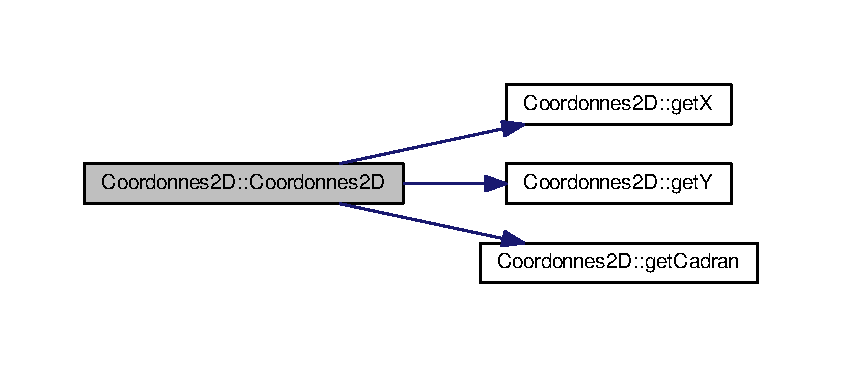
\includegraphics[width=350pt]{class_coordonnes2_d_a32915a0b2cfc5dce3ed491fb3fa0abae_cgraph}
\end{center}
\end{figure}


\index{Coordonnes2\-D@{Coordonnes2\-D}!$\sim$\-Coordonnes2\-D@{$\sim$\-Coordonnes2\-D}}
\index{$\sim$\-Coordonnes2\-D@{$\sim$\-Coordonnes2\-D}!Coordonnes2D@{Coordonnes2\-D}}
\subsubsection[{$\sim$\-Coordonnes2\-D}]{\setlength{\rightskip}{0pt plus 5cm}Coordonnes2\-D\-::$\sim$\-Coordonnes2\-D (
\begin{DoxyParamCaption}
{}
\end{DoxyParamCaption}
)\hspace{0.3cm}{\ttfamily [virtual]}}\label{class_coordonnes2_d_a65b01695cc5bd68968db3ded7a1fcf74}


Destructeur. 

Default destructor

Destructeur de la classe \doxyref{Coordonnes2\-D}{p.}{class_coordonnes2_d} 

\subsection{Documentation des fonctions membres}
\index{Coordonnes2\-D@{Coordonnes2\-D}!get\-Cadran@{get\-Cadran}}
\index{get\-Cadran@{get\-Cadran}!Coordonnes2D@{Coordonnes2\-D}}
\subsubsection[{get\-Cadran}]{\setlength{\rightskip}{0pt plus 5cm}int Coordonnes2\-D\-::get\-Cadran (
\begin{DoxyParamCaption}
{}
\end{DoxyParamCaption}
) const\hspace{0.3cm}{\ttfamily [inline]}}\label{class_coordonnes2_d_a923a832cec319899e4435240e1d1a2ce}


Getter. 

Getter de l'attribut m\-\_\-cadran de la classe \doxyref{Coordonnes2\-D}{p.}{class_coordonnes2_d}

\begin{DoxyReturn}{Renvoie}
l'attribut m\-\_\-cadran de la classe \doxyref{Coordonnes2\-D}{p.}{class_coordonnes2_d} 
\end{DoxyReturn}


Voici le graphe des appelants de cette fonction \-:
\nopagebreak
\begin{figure}[H]
\begin{center}
\leavevmode
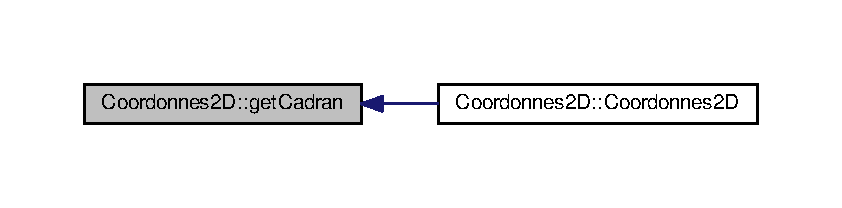
\includegraphics[width=350pt]{class_coordonnes2_d_a923a832cec319899e4435240e1d1a2ce_icgraph}
\end{center}
\end{figure}


\index{Coordonnes2\-D@{Coordonnes2\-D}!get\-X@{get\-X}}
\index{get\-X@{get\-X}!Coordonnes2D@{Coordonnes2\-D}}
\subsubsection[{get\-X}]{\setlength{\rightskip}{0pt plus 5cm}int Coordonnes2\-D\-::get\-X (
\begin{DoxyParamCaption}
{}
\end{DoxyParamCaption}
) const\hspace{0.3cm}{\ttfamily [inline]}}\label{class_coordonnes2_d_ac06b44e9c6584d4de6746f6b14472cdb}


Getter. 

Getter de l'attribut m\-\_\-\-X de la classe \doxyref{Coordonnes2\-D}{p.}{class_coordonnes2_d}

\begin{DoxyReturn}{Renvoie}
l'attribut m\-\_\-\-X de la classe \doxyref{Coordonnes2\-D}{p.}{class_coordonnes2_d} 
\end{DoxyReturn}


Voici le graphe des appelants de cette fonction \-:
\nopagebreak
\begin{figure}[H]
\begin{center}
\leavevmode
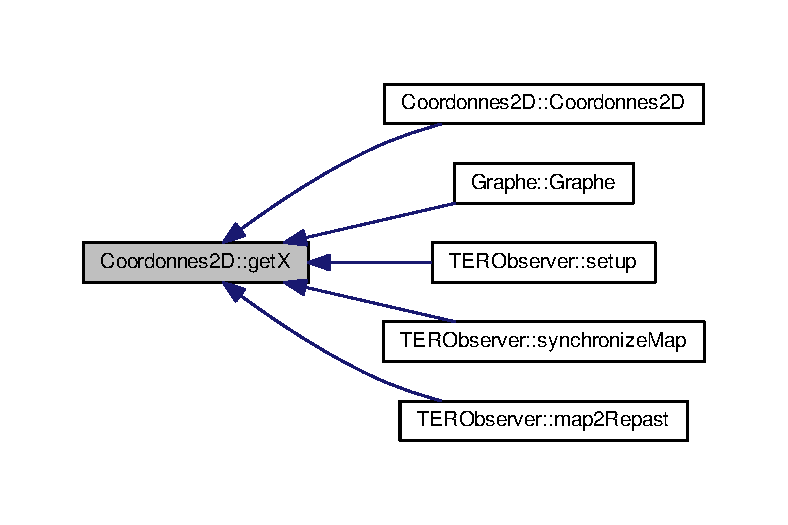
\includegraphics[width=350pt]{class_coordonnes2_d_ac06b44e9c6584d4de6746f6b14472cdb_icgraph}
\end{center}
\end{figure}


\index{Coordonnes2\-D@{Coordonnes2\-D}!get\-Y@{get\-Y}}
\index{get\-Y@{get\-Y}!Coordonnes2D@{Coordonnes2\-D}}
\subsubsection[{get\-Y}]{\setlength{\rightskip}{0pt plus 5cm}int Coordonnes2\-D\-::get\-Y (
\begin{DoxyParamCaption}
{}
\end{DoxyParamCaption}
) const\hspace{0.3cm}{\ttfamily [inline]}}\label{class_coordonnes2_d_a52192f87a21074e41b7d7b22f258a549}


Getter. 

Getter de l'attribut m\-\_\-\-Y de la classe \doxyref{Coordonnes2\-D}{p.}{class_coordonnes2_d}

\begin{DoxyReturn}{Renvoie}
l'attribut m\-\_\-\-Y de la classe \doxyref{Coordonnes2\-D}{p.}{class_coordonnes2_d} 
\end{DoxyReturn}


Voici le graphe des appelants de cette fonction \-:
\nopagebreak
\begin{figure}[H]
\begin{center}
\leavevmode
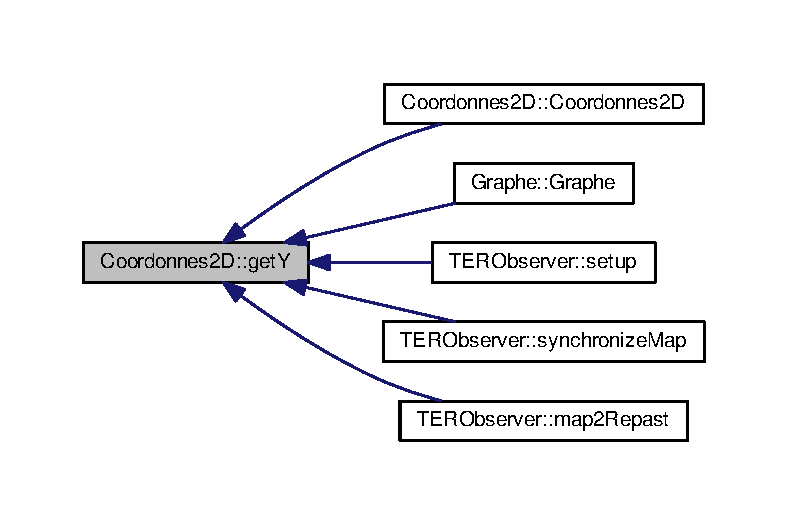
\includegraphics[width=350pt]{class_coordonnes2_d_a52192f87a21074e41b7d7b22f258a549_icgraph}
\end{center}
\end{figure}


\index{Coordonnes2\-D@{Coordonnes2\-D}!set\-Cadran@{set\-Cadran}}
\index{set\-Cadran@{set\-Cadran}!Coordonnes2D@{Coordonnes2\-D}}
\subsubsection[{set\-Cadran}]{\setlength{\rightskip}{0pt plus 5cm}void Coordonnes2\-D\-::set\-Cadran (
\begin{DoxyParamCaption}
\item[{int}]{val}
\end{DoxyParamCaption}
)\hspace{0.3cm}{\ttfamily [inline]}}\label{class_coordonnes2_d_a83505a182e95dee074796050f5fc960b}


Setter. 

Setter de l'attribut m\-\_\-cadran de la classe \doxyref{Coordonnes2\-D}{p.}{class_coordonnes2_d} \index{Coordonnes2\-D@{Coordonnes2\-D}!set\-X@{set\-X}}
\index{set\-X@{set\-X}!Coordonnes2D@{Coordonnes2\-D}}
\subsubsection[{set\-X}]{\setlength{\rightskip}{0pt plus 5cm}void Coordonnes2\-D\-::set\-X (
\begin{DoxyParamCaption}
\item[{int}]{X}
\end{DoxyParamCaption}
)\hspace{0.3cm}{\ttfamily [inline]}}\label{class_coordonnes2_d_acd18a61d429f17132bd6af7c66c5f56d}


Setter. 

Setter de l'attribut m\-\_\-\-X de la classe \doxyref{Coordonnes2\-D}{p.}{class_coordonnes2_d} 

Voici le graphe des appelants de cette fonction \-:
\nopagebreak
\begin{figure}[H]
\begin{center}
\leavevmode
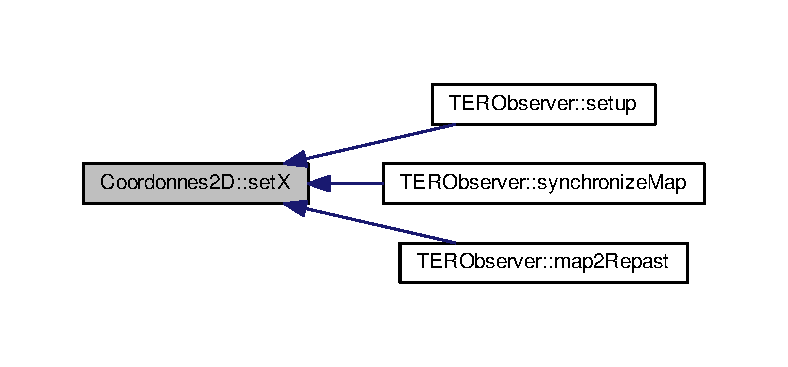
\includegraphics[width=350pt]{class_coordonnes2_d_acd18a61d429f17132bd6af7c66c5f56d_icgraph}
\end{center}
\end{figure}


\index{Coordonnes2\-D@{Coordonnes2\-D}!set\-Y@{set\-Y}}
\index{set\-Y@{set\-Y}!Coordonnes2D@{Coordonnes2\-D}}
\subsubsection[{set\-Y}]{\setlength{\rightskip}{0pt plus 5cm}void Coordonnes2\-D\-::set\-Y (
\begin{DoxyParamCaption}
\item[{int}]{Y}
\end{DoxyParamCaption}
)\hspace{0.3cm}{\ttfamily [inline]}}\label{class_coordonnes2_d_a1b611c902888fced2b0712ed6e84a3fb}


Setter. 

Setter de l'attribut m\-\_\-\-Y de la classe \doxyref{Coordonnes2\-D}{p.}{class_coordonnes2_d} 

Voici le graphe des appelants de cette fonction \-:
\nopagebreak
\begin{figure}[H]
\begin{center}
\leavevmode
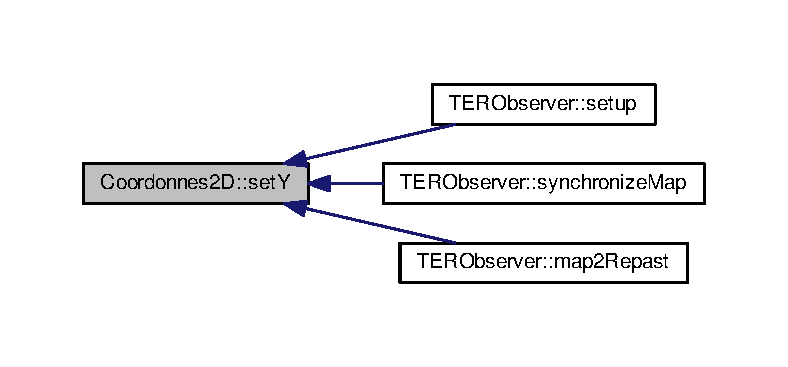
\includegraphics[width=350pt]{class_coordonnes2_d_a1b611c902888fced2b0712ed6e84a3fb_icgraph}
\end{center}
\end{figure}




\subsection{Documentation des données membres}
\index{Coordonnes2\-D@{Coordonnes2\-D}!m\-\_\-cadran@{m\-\_\-cadran}}
\index{m\-\_\-cadran@{m\-\_\-cadran}!Coordonnes2D@{Coordonnes2\-D}}
\subsubsection[{m\-\_\-cadran}]{\setlength{\rightskip}{0pt plus 5cm}int Coordonnes2\-D\-::m\-\_\-cadran\hspace{0.3cm}{\ttfamily [protected]}}\label{class_coordonnes2_d_ad09082ceb0a4e3ea127ff78192a58a68}
cadran de la fenetre \index{Coordonnes2\-D@{Coordonnes2\-D}!m\-\_\-\-X@{m\-\_\-\-X}}
\index{m\-\_\-\-X@{m\-\_\-\-X}!Coordonnes2D@{Coordonnes2\-D}}
\subsubsection[{m\-\_\-\-X}]{\setlength{\rightskip}{0pt plus 5cm}int Coordonnes2\-D\-::m\-\_\-\-X\hspace{0.3cm}{\ttfamily [protected]}}\label{class_coordonnes2_d_a27d023c95955192562e88d8dcb3550ea}
position X \index{Coordonnes2\-D@{Coordonnes2\-D}!m\-\_\-\-Y@{m\-\_\-\-Y}}
\index{m\-\_\-\-Y@{m\-\_\-\-Y}!Coordonnes2D@{Coordonnes2\-D}}
\subsubsection[{m\-\_\-\-Y}]{\setlength{\rightskip}{0pt plus 5cm}int Coordonnes2\-D\-::m\-\_\-\-Y\hspace{0.3cm}{\ttfamily [protected]}}\label{class_coordonnes2_d_aaae6b7822c9680973ad6e55255ffa45a}
position Y 

La documentation de cette classe a été générée à partir des fichiers suivants \-:\begin{DoxyCompactItemize}
\item 
code/include/{\bf coordonnes2d.\-h}\item 
code/src/coordonnes2d.\-cpp\end{DoxyCompactItemize}

\section{Référence de la classe Couleur}
\label{class_couleur}\index{Couleur@{Couleur}}


Classe representant une \doxyref{Couleur}{p.}{class_couleur}.  




{\ttfamily \#include $<$couleur.\-h$>$}

\subsection*{Fonctions membres publiques}
\begin{DoxyCompactItemize}
\item 
{\bf Couleur} (Uint8 R, Uint8 G, Uint8 B)
\begin{DoxyCompactList}\small\item\em Constructeur. \end{DoxyCompactList}\item 
virtual {\bf $\sim$\-Couleur} ()
\begin{DoxyCompactList}\small\item\em Destructeur. \end{DoxyCompactList}\item 
Uint32 {\bf get\-Color} ()
\begin{DoxyCompactList}\small\item\em Getter. \end{DoxyCompactList}\item 
S\-D\-L\-\_\-\-Color {\bf get\-S\-D\-L\-Color} ()
\begin{DoxyCompactList}\small\item\em Getter. \end{DoxyCompactList}\item 
Uint8 {\bf get\-R} ()
\begin{DoxyCompactList}\small\item\em Getter. \end{DoxyCompactList}\item 
Uint8 {\bf get\-G} ()
\begin{DoxyCompactList}\small\item\em Getter. \end{DoxyCompactList}\item 
Uint8 {\bf get\-B} ()
\begin{DoxyCompactList}\small\item\em Getter. \end{DoxyCompactList}\item 
void {\bf set\-Color} (Uint32 val)
\begin{DoxyCompactList}\small\item\em Setter. \end{DoxyCompactList}\item 
void {\bf set\-S\-D\-L\-Color} (S\-D\-L\-\_\-\-Color val)
\begin{DoxyCompactList}\small\item\em Setter. \end{DoxyCompactList}\item 
void {\bf set\-R} (Uint8 val)
\begin{DoxyCompactList}\small\item\em Setter. \end{DoxyCompactList}\item 
void {\bf set\-G} (Uint8 val)
\begin{DoxyCompactList}\small\item\em Setter. \end{DoxyCompactList}\item 
void {\bf set\-B} (Uint8 val)
\begin{DoxyCompactList}\small\item\em Setter. \end{DoxyCompactList}\item 
void {\bf set\-R\-G\-B} (Uint8 val\-R, Uint8 val\-G, Uint8 val\-B)
\begin{DoxyCompactList}\small\item\em Setter. \end{DoxyCompactList}\end{DoxyCompactItemize}
\subsection*{Attributs protégés}
\begin{DoxyCompactItemize}
\item 
Uint8 {\bf m\-\_\-\-R}
\item 
Uint8 {\bf m\-\_\-\-G}
\item 
Uint8 {\bf m\-\_\-\-B}
\item 
S\-D\-L\-\_\-\-Color {\bf m\-\_\-color}
\item 
Uint32 {\bf m\-\_\-color\-\_\-uint32}
\end{DoxyCompactItemize}


\subsection{Description détaillée}
Classe representant une \doxyref{Couleur}{p.}{class_couleur}. 

La classe est composee des des quantité de Rouge, Vert et Bleu d'une couleur. 

\subsection{Documentation des constructeurs et destructeur}
\index{Couleur@{Couleur}!Couleur@{Couleur}}
\index{Couleur@{Couleur}!Couleur@{Couleur}}
\subsubsection[{Couleur}]{\setlength{\rightskip}{0pt plus 5cm}Couleur\-::\-Couleur (
\begin{DoxyParamCaption}
\item[{Uint8}]{R, }
\item[{Uint8}]{G, }
\item[{Uint8}]{B}
\end{DoxyParamCaption}
)}\label{class_couleur_a76e1f4a1d806979e4b9cda22544e43de}


Constructeur. 

Default constructor

Constructeur de la classe \doxyref{Couleur}{p.}{class_couleur}


\begin{DoxyParams}{Paramètres}
{\em R} & \-: quantite de rouge \\
\hline
{\em G} & \-: quantite de vert \\
\hline
{\em B} & \-: quantite de bleu \\
\hline
\end{DoxyParams}
\index{Couleur@{Couleur}!$\sim$\-Couleur@{$\sim$\-Couleur}}
\index{$\sim$\-Couleur@{$\sim$\-Couleur}!Couleur@{Couleur}}
\subsubsection[{$\sim$\-Couleur}]{\setlength{\rightskip}{0pt plus 5cm}Couleur\-::$\sim$\-Couleur (
\begin{DoxyParamCaption}
{}
\end{DoxyParamCaption}
)\hspace{0.3cm}{\ttfamily [virtual]}}\label{class_couleur_ad3be30be83649bc5db48ef46b592aec2}


Destructeur. 

Destructeur de la classe \doxyref{Couleur}{p.}{class_couleur} 

\subsection{Documentation des fonctions membres}
\index{Couleur@{Couleur}!get\-B@{get\-B}}
\index{get\-B@{get\-B}!Couleur@{Couleur}}
\subsubsection[{get\-B}]{\setlength{\rightskip}{0pt plus 5cm}Uint8 Couleur\-::get\-B (
\begin{DoxyParamCaption}
{}
\end{DoxyParamCaption}
)}\label{class_couleur_ab023b75cf9580d1f3071f8426030add7}


Getter. 

Getter de l'attribut m\-\_\-\-B de la classe \doxyref{Couleur}{p.}{class_couleur} 

Voici le graphe des appelants de cette fonction \-:
\nopagebreak
\begin{figure}[H]
\begin{center}
\leavevmode
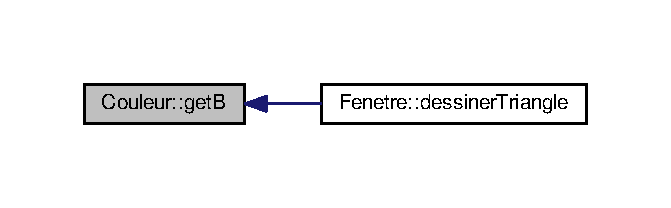
\includegraphics[width=322pt]{class_couleur_ab023b75cf9580d1f3071f8426030add7_icgraph}
\end{center}
\end{figure}


\index{Couleur@{Couleur}!get\-Color@{get\-Color}}
\index{get\-Color@{get\-Color}!Couleur@{Couleur}}
\subsubsection[{get\-Color}]{\setlength{\rightskip}{0pt plus 5cm}Uint32 Couleur\-::get\-Color (
\begin{DoxyParamCaption}
{}
\end{DoxyParamCaption}
)}\label{class_couleur_ac0aac7fb19221ae95f260a319417f0bc}


Getter. 

Getters

Getter de l'attribut m\-\_\-color\-\_\-uint32 de la classe \doxyref{Couleur}{p.}{class_couleur}

Getters \index{Couleur@{Couleur}!get\-G@{get\-G}}
\index{get\-G@{get\-G}!Couleur@{Couleur}}
\subsubsection[{get\-G}]{\setlength{\rightskip}{0pt plus 5cm}Uint8 Couleur\-::get\-G (
\begin{DoxyParamCaption}
{}
\end{DoxyParamCaption}
)}\label{class_couleur_a93a7af80f901c100e59eca533f4be51c}


Getter. 

Getter de l'attribut m\-\_\-\-G de la classe \doxyref{Couleur}{p.}{class_couleur} 

Voici le graphe des appelants de cette fonction \-:
\nopagebreak
\begin{figure}[H]
\begin{center}
\leavevmode
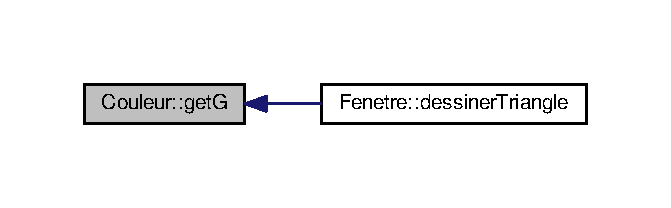
\includegraphics[width=322pt]{class_couleur_a93a7af80f901c100e59eca533f4be51c_icgraph}
\end{center}
\end{figure}


\index{Couleur@{Couleur}!get\-R@{get\-R}}
\index{get\-R@{get\-R}!Couleur@{Couleur}}
\subsubsection[{get\-R}]{\setlength{\rightskip}{0pt plus 5cm}Uint8 Couleur\-::get\-R (
\begin{DoxyParamCaption}
{}
\end{DoxyParamCaption}
)}\label{class_couleur_a5180881bc65a09404e3574041039c71b}


Getter. 

Getter de l'attribut m\-\_\-\-R de la classe \doxyref{Couleur}{p.}{class_couleur} 

Voici le graphe des appelants de cette fonction \-:
\nopagebreak
\begin{figure}[H]
\begin{center}
\leavevmode
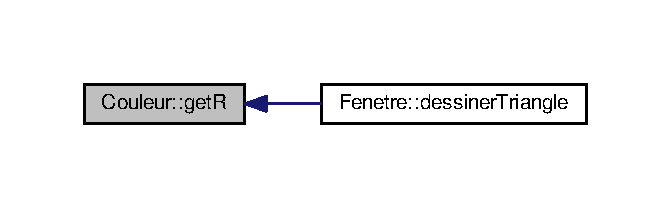
\includegraphics[width=322pt]{class_couleur_a5180881bc65a09404e3574041039c71b_icgraph}
\end{center}
\end{figure}


\index{Couleur@{Couleur}!get\-S\-D\-L\-Color@{get\-S\-D\-L\-Color}}
\index{get\-S\-D\-L\-Color@{get\-S\-D\-L\-Color}!Couleur@{Couleur}}
\subsubsection[{get\-S\-D\-L\-Color}]{\setlength{\rightskip}{0pt plus 5cm}S\-D\-L\-\_\-\-Color Couleur\-::get\-S\-D\-L\-Color (
\begin{DoxyParamCaption}
{}
\end{DoxyParamCaption}
)}\label{class_couleur_a1aaf4c0ae55292079975733a9a356549}


Getter. 

Getter de l'attribut m\-\_\-color de la classe \doxyref{Couleur}{p.}{class_couleur} \index{Couleur@{Couleur}!set\-B@{set\-B}}
\index{set\-B@{set\-B}!Couleur@{Couleur}}
\subsubsection[{set\-B}]{\setlength{\rightskip}{0pt plus 5cm}void Couleur\-::set\-B (
\begin{DoxyParamCaption}
\item[{Uint8}]{val}
\end{DoxyParamCaption}
)}\label{class_couleur_abfb5df8e05b8bed718c778b5c3805b82}


Setter. 

Setter de l'attribut m\-\_\-\-B de la classe \doxyref{Couleur}{p.}{class_couleur} 
\begin{DoxyParams}{Paramètres}
{\em val} & \-: valeur a attribuer a l'attribut m\-\_\-\-B de la classe \doxyref{Couleur}{p.}{class_couleur} \\
\hline
\end{DoxyParams}
\index{Couleur@{Couleur}!set\-Color@{set\-Color}}
\index{set\-Color@{set\-Color}!Couleur@{Couleur}}
\subsubsection[{set\-Color}]{\setlength{\rightskip}{0pt plus 5cm}void Couleur\-::set\-Color (
\begin{DoxyParamCaption}
\item[{Uint32}]{val}
\end{DoxyParamCaption}
)}\label{class_couleur_a3cb04e618c052235b4f346c4b12a9090}


Setter. 

Setters

Setter de l'attribut m\-\_\-color\-\_\-uint32 de la classe \doxyref{Couleur}{p.}{class_couleur} 
\begin{DoxyParams}{Paramètres}
{\em val} & \-: valeur a attribuer a l'attribut m\-\_\-color\-\_\-uint32 de la classe \doxyref{Couleur}{p.}{class_couleur}\\
\hline
\end{DoxyParams}
Setters \index{Couleur@{Couleur}!set\-G@{set\-G}}
\index{set\-G@{set\-G}!Couleur@{Couleur}}
\subsubsection[{set\-G}]{\setlength{\rightskip}{0pt plus 5cm}void Couleur\-::set\-G (
\begin{DoxyParamCaption}
\item[{Uint8}]{val}
\end{DoxyParamCaption}
)}\label{class_couleur_a9daf9b524e96bd6ab7a47f7f04918bf6}


Setter. 

Setter de l'attribut m\-\_\-\-G de la classe \doxyref{Couleur}{p.}{class_couleur} 
\begin{DoxyParams}{Paramètres}
{\em val} & \-: valeur a attribuer a l'attribut m\-\_\-\-G de la classe \doxyref{Couleur}{p.}{class_couleur} \\
\hline
\end{DoxyParams}
\index{Couleur@{Couleur}!set\-R@{set\-R}}
\index{set\-R@{set\-R}!Couleur@{Couleur}}
\subsubsection[{set\-R}]{\setlength{\rightskip}{0pt plus 5cm}void Couleur\-::set\-R (
\begin{DoxyParamCaption}
\item[{Uint8}]{val}
\end{DoxyParamCaption}
)}\label{class_couleur_a4528e835d33d36f9a572aede35af2dc8}


Setter. 

Setter de l'attribut m\-\_\-\-R de la classe \doxyref{Couleur}{p.}{class_couleur} 
\begin{DoxyParams}{Paramètres}
{\em val} & \-: valeur a attribuer a l'attribut m\-\_\-\-R de la classe \doxyref{Couleur}{p.}{class_couleur} \\
\hline
\end{DoxyParams}
\index{Couleur@{Couleur}!set\-R\-G\-B@{set\-R\-G\-B}}
\index{set\-R\-G\-B@{set\-R\-G\-B}!Couleur@{Couleur}}
\subsubsection[{set\-R\-G\-B}]{\setlength{\rightskip}{0pt plus 5cm}void Couleur\-::set\-R\-G\-B (
\begin{DoxyParamCaption}
\item[{Uint8}]{val\-R, }
\item[{Uint8}]{val\-G, }
\item[{Uint8}]{val\-B}
\end{DoxyParamCaption}
)}\label{class_couleur_a052ee51440843dbd62c6ee58bcfd657e}


Setter. 

Setter des attributs m\-\_\-\-R , m\-\_\-\-G , m\-\_\-\-B de la classe \doxyref{Couleur}{p.}{class_couleur} 
\begin{DoxyParams}{Paramètres}
{\em val\-R} & \-: valeur a attribuer a l'attribut m\-\_\-\-R de la classe \doxyref{Couleur}{p.}{class_couleur} \\
\hline
{\em val\-G} & \-: valeur a attribuer a l'attribut m\-\_\-\-G de la classe \doxyref{Couleur}{p.}{class_couleur} \\
\hline
{\em val\-B} & \-: valeur a attribuer a l'attribut m\-\_\-\-B de la classe \doxyref{Couleur}{p.}{class_couleur} \\
\hline
\end{DoxyParams}
\index{Couleur@{Couleur}!set\-S\-D\-L\-Color@{set\-S\-D\-L\-Color}}
\index{set\-S\-D\-L\-Color@{set\-S\-D\-L\-Color}!Couleur@{Couleur}}
\subsubsection[{set\-S\-D\-L\-Color}]{\setlength{\rightskip}{0pt plus 5cm}void Couleur\-::set\-S\-D\-L\-Color (
\begin{DoxyParamCaption}
\item[{S\-D\-L\-\_\-\-Color}]{val}
\end{DoxyParamCaption}
)}\label{class_couleur_ad47eb978662052be6e123a937a9ef962}


Setter. 

Setter de l'attribut m\-\_\-color de la classe \doxyref{Couleur}{p.}{class_couleur} 
\begin{DoxyParams}{Paramètres}
{\em val} & \-: valeur a attribuer a l'attribut m\-\_\-color de la classe \doxyref{Couleur}{p.}{class_couleur} \\
\hline
\end{DoxyParams}


\subsection{Documentation des données membres}
\index{Couleur@{Couleur}!m\-\_\-\-B@{m\-\_\-\-B}}
\index{m\-\_\-\-B@{m\-\_\-\-B}!Couleur@{Couleur}}
\subsubsection[{m\-\_\-\-B}]{\setlength{\rightskip}{0pt plus 5cm}Uint8 Couleur\-::m\-\_\-\-B\hspace{0.3cm}{\ttfamily [protected]}}\label{class_couleur_aecca85052daa7d274054e6b596ef45f9}
quantite de bleu \index{Couleur@{Couleur}!m\-\_\-color@{m\-\_\-color}}
\index{m\-\_\-color@{m\-\_\-color}!Couleur@{Couleur}}
\subsubsection[{m\-\_\-color}]{\setlength{\rightskip}{0pt plus 5cm}S\-D\-L\-\_\-\-Color Couleur\-::m\-\_\-color\hspace{0.3cm}{\ttfamily [protected]}}\label{class_couleur_a79655eaff895eb4660f5e5f2de29219d}
structure de donnee S\-D\-L pour representer une couleur \index{Couleur@{Couleur}!m\-\_\-color\-\_\-uint32@{m\-\_\-color\-\_\-uint32}}
\index{m\-\_\-color\-\_\-uint32@{m\-\_\-color\-\_\-uint32}!Couleur@{Couleur}}
\subsubsection[{m\-\_\-color\-\_\-uint32}]{\setlength{\rightskip}{0pt plus 5cm}Uint32 Couleur\-::m\-\_\-color\-\_\-uint32\hspace{0.3cm}{\ttfamily [protected]}}\label{class_couleur_a058a61c5628ab35f9460f1c7448a459a}
structure de donnee S\-D\-L pour representer une couleur \index{Couleur@{Couleur}!m\-\_\-\-G@{m\-\_\-\-G}}
\index{m\-\_\-\-G@{m\-\_\-\-G}!Couleur@{Couleur}}
\subsubsection[{m\-\_\-\-G}]{\setlength{\rightskip}{0pt plus 5cm}Uint8 Couleur\-::m\-\_\-\-G\hspace{0.3cm}{\ttfamily [protected]}}\label{class_couleur_a8f94550905b39dd43c5996eefb452c9c}
quantite de vert \index{Couleur@{Couleur}!m\-\_\-\-R@{m\-\_\-\-R}}
\index{m\-\_\-\-R@{m\-\_\-\-R}!Couleur@{Couleur}}
\subsubsection[{m\-\_\-\-R}]{\setlength{\rightskip}{0pt plus 5cm}Uint8 Couleur\-::m\-\_\-\-R\hspace{0.3cm}{\ttfamily [protected]}}\label{class_couleur_a15547a9f64d343ad8f1482acd09a4c2f}
quantite de rouge 

La documentation de cette classe a été générée à partir des fichiers suivants \-:\begin{DoxyCompactItemize}
\item 
code/include/{\bf couleur.\-h}\item 
code/src/couleur.\-cpp\end{DoxyCompactItemize}

\section{Référence de la classe Fenetre}
\label{class_fenetre}\index{Fenetre@{Fenetre}}


Classe representant une \doxyref{Fenetre}{p.}{class_fenetre} S\-D\-L.  




{\ttfamily \#include $<$fenetre.\-h$>$}

\subsection*{Fonctions membres publiques}
\begin{DoxyCompactItemize}
\item 
{\bf Fenetre} (std\-::string titre, boost\-::mpi\-::communicator $\ast${\bf world}, unsigned int cadran, unsigned int longueur=400, unsigned int hauteur=400)
\begin{DoxyCompactList}\small\item\em Constructeur. \end{DoxyCompactList}\item 
virtual {\bf $\sim$\-Fenetre} ()
\item 
void {\bfseries main\-\_\-loop} ()\label{class_fenetre_a2e1f40693f1610ec445296665e0504af}

\item 
void {\bf refresh} (void)
\begin{DoxyCompactList}\small\item\em rafraichissement de la fenetre \end{DoxyCompactList}\item 
unsigned int {\bf get\-Longueur} ()
\begin{DoxyCompactList}\small\item\em Getter de l'attribut m\-\_\-largeur de la classe \doxyref{Fenetre}{p.}{class_fenetre}. \end{DoxyCompactList}\item 
unsigned int {\bf get\-Hauteur} ()
\begin{DoxyCompactList}\small\item\em Getter de l'attribut m\-\_\-hauteur de la classe \doxyref{Fenetre}{p.}{class_fenetre}. \end{DoxyCompactList}\item 
void {\bf dessiner\-Triangle} (int pos\-X, int pos\-Y, double angle, int type)
\begin{DoxyCompactList}\small\item\em fonction qui dessine un triangle sur la fenetre \end{DoxyCompactList}\item 
void {\bf dessiner\-Mur} (int pos\-X, int pos\-Y)
\begin{DoxyCompactList}\small\item\em fonction qui dessine un carré 20x20 pixels (\doxyref{Mur}{p.}{class_mur}) sur la fenetre \end{DoxyCompactList}\item 
S\-D\-L\-\_\-\-Window $\ast$ {\bf get\-Screen} ()
\begin{DoxyCompactList}\small\item\em Getter de l'attribut m\-\_\-ecran de la classe \doxyref{Fenetre}{p.}{class_fenetre}. \end{DoxyCompactList}\item 
S\-D\-L\-\_\-\-G\-L\-Context {\bf get\-G\-L\-Context} ()
\begin{DoxyCompactList}\small\item\em Getter de l'attribut m\-\_\-context de la classe \doxyref{Fenetre}{p.}{class_fenetre}. \end{DoxyCompactList}\item 
int {\bf get\-Cadran} ()
\begin{DoxyCompactList}\small\item\em Getter de l'attribut m\-\_\-cadran de la classe \doxyref{Fenetre}{p.}{class_fenetre}. \end{DoxyCompactList}\item 
void {\bf clear} (void)\label{class_fenetre_a1ca0cdad76751701230756f891e1c1be}

\begin{DoxyCompactList}\small\item\em fonction qui redessine en blanc la fenetre (effacement) \end{DoxyCompactList}\item 
void {\bf dormir} (int val)
\begin{DoxyCompactList}\small\item\em fonction qui endors le processus qui s'occupe de la fenetre \end{DoxyCompactList}\end{DoxyCompactItemize}
\subsection*{Attributs protégés}
\begin{DoxyCompactItemize}
\item 
boost\-::mpi\-::communicator $\ast$ {\bf world}
\item 
unsigned int {\bf m\-\_\-largeur}
\item 
unsigned int {\bf m\-\_\-hauteur}
\item 
unsigned int {\bf m\-\_\-cadran}
\item 
std\-::string {\bf m\-\_\-titre}
\item 
S\-D\-L\-\_\-\-Window $\ast$ {\bf m\-\_\-ecran}
\item 
S\-D\-L\-\_\-\-G\-L\-Context {\bf m\-\_\-context}
\item 
Uint32 {\bf m\-\_\-bg\-\_\-color}
\item 
S\-D\-L\-\_\-\-Event {\bf m\-\_\-e}
\end{DoxyCompactItemize}


\subsection{Description détaillée}
Classe representant une \doxyref{Fenetre}{p.}{class_fenetre} S\-D\-L. 

La classe est composee des dimensions de la fentre, du titre, du cadran auquel elle appartient, un communicateur avec les autres processus. 

\subsection{Documentation des constructeurs et destructeur}
\index{Fenetre@{Fenetre}!Fenetre@{Fenetre}}
\index{Fenetre@{Fenetre}!Fenetre@{Fenetre}}
\subsubsection[{Fenetre}]{\setlength{\rightskip}{0pt plus 5cm}Fenetre\-::\-Fenetre (
\begin{DoxyParamCaption}
\item[{std\-::string}]{titre, }
\item[{boost\-::mpi\-::communicator $\ast$}]{world, }
\item[{unsigned int}]{cadran, }
\item[{unsigned int}]{longueur = {\ttfamily 400}, }
\item[{unsigned int}]{hauteur = {\ttfamily 400}}
\end{DoxyParamCaption}
)}\label{class_fenetre_a541961b7302c76d76a2db26ba6d75ecd}


Constructeur. 

Default constructor

Constructeur de la classe \doxyref{Fenetre}{p.}{class_fenetre}


\begin{DoxyParams}{Paramètres}
{\em world} & \-: canal de communication avec les autres processus \\
\hline
{\em cadran} & \-: numero de cadran du monde dont s'occupe le processus qui contient la fenetre \\
\hline
{\em longueur} & \-: longueur de la fenetre en pixels(400 par default) \\
\hline
{\em hauteur} & \-: hauteur de la fenetre en pixels(400 par default) \\
\hline
\end{DoxyParams}
\index{Fenetre@{Fenetre}!$\sim$\-Fenetre@{$\sim$\-Fenetre}}
\index{$\sim$\-Fenetre@{$\sim$\-Fenetre}!Fenetre@{Fenetre}}
\subsubsection[{$\sim$\-Fenetre}]{\setlength{\rightskip}{0pt plus 5cm}Fenetre\-::$\sim$\-Fenetre (
\begin{DoxyParamCaption}
{}
\end{DoxyParamCaption}
)\hspace{0.3cm}{\ttfamily [virtual]}}\label{class_fenetre_a4738cb1dcb874908428b66b5ecd794c4}
Default destructor 

\subsection{Documentation des fonctions membres}
\index{Fenetre@{Fenetre}!dessiner\-Mur@{dessiner\-Mur}}
\index{dessiner\-Mur@{dessiner\-Mur}!Fenetre@{Fenetre}}
\subsubsection[{dessiner\-Mur}]{\setlength{\rightskip}{0pt plus 5cm}void Fenetre\-::dessiner\-Mur (
\begin{DoxyParamCaption}
\item[{int}]{pos\-X, }
\item[{int}]{pos\-Y}
\end{DoxyParamCaption}
)}\label{class_fenetre_a7f2786a8441da33363c05fbcd0cdb4af}


fonction qui dessine un carré 20x20 pixels (\doxyref{Mur}{p.}{class_mur}) sur la fenetre 


\begin{DoxyParams}{Paramètres}
{\em pos\-X} & \-: position X ou l'on veut dessiner le mur \\
\hline
{\em pos\-Y} & \-: position Y ou l'on veut dessiner le mur \\
\hline
\end{DoxyParams}
\index{Fenetre@{Fenetre}!dessiner\-Triangle@{dessiner\-Triangle}}
\index{dessiner\-Triangle@{dessiner\-Triangle}!Fenetre@{Fenetre}}
\subsubsection[{dessiner\-Triangle}]{\setlength{\rightskip}{0pt plus 5cm}void Fenetre\-::dessiner\-Triangle (
\begin{DoxyParamCaption}
\item[{int}]{pos\-X, }
\item[{int}]{pos\-Y, }
\item[{double}]{angle, }
\item[{int}]{type}
\end{DoxyParamCaption}
)}\label{class_fenetre_a13c7ea9a022308e15be7bd3e74c7b30f}


fonction qui dessine un triangle sur la fenetre 


\begin{DoxyParams}{Paramètres}
{\em pos\-X} & \-: position X du centre de gravite du triangle a dessiner \\
\hline
{\em pos\-Y} & \-: position Y du centre de gravite du triangle a dessiner \\
\hline
{\em pos\-X} & \-: valeur de l'angle en degre duquel on doit faire pivoter le triangle (sens trigo) \\
\hline
{\em type} & \-: couleur du triangle a dessiner selon le type (A\-D\-U\-L\-T\-E, J\-E\-U\-N\-E , P\-E\-R\-S\-O\-N\-N\-E A\-G\-E\-E ou M\-A\-L\-A\-D\-E) \\
\hline
\end{DoxyParams}


Voici le graphe d'appel pour cette fonction \-:
\nopagebreak
\begin{figure}[H]
\begin{center}
\leavevmode
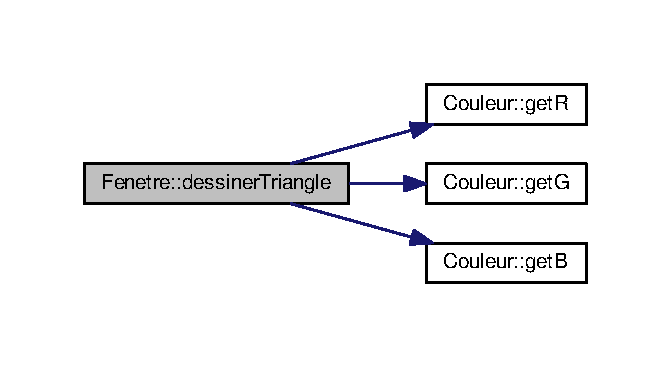
\includegraphics[width=322pt]{class_fenetre_a13c7ea9a022308e15be7bd3e74c7b30f_cgraph}
\end{center}
\end{figure}


\index{Fenetre@{Fenetre}!dormir@{dormir}}
\index{dormir@{dormir}!Fenetre@{Fenetre}}
\subsubsection[{dormir}]{\setlength{\rightskip}{0pt plus 5cm}void Fenetre\-::dormir (
\begin{DoxyParamCaption}
\item[{int}]{val}
\end{DoxyParamCaption}
)}\label{class_fenetre_a51514f010265cc7fda442f3d6e38e019}


fonction qui endors le processus qui s'occupe de la fenetre 


\begin{DoxyParams}{Paramètres}
{\em val} & \-: valeur en millisecondes durant laquelle le processus doit s'endormir \\
\hline
\end{DoxyParams}
\index{Fenetre@{Fenetre}!get\-Cadran@{get\-Cadran}}
\index{get\-Cadran@{get\-Cadran}!Fenetre@{Fenetre}}
\subsubsection[{get\-Cadran}]{\setlength{\rightskip}{0pt plus 5cm}int Fenetre\-::get\-Cadran (
\begin{DoxyParamCaption}
{}
\end{DoxyParamCaption}
)}\label{class_fenetre_ac9b0a5adee0900502417cee80a0d3fc2}


Getter de l'attribut m\-\_\-cadran de la classe \doxyref{Fenetre}{p.}{class_fenetre}. 

\begin{DoxyReturn}{Renvoie}
valeur de l'attribut m\-\_\-cadran de la classe \doxyref{Fenetre}{p.}{class_fenetre} 
\end{DoxyReturn}
\index{Fenetre@{Fenetre}!get\-G\-L\-Context@{get\-G\-L\-Context}}
\index{get\-G\-L\-Context@{get\-G\-L\-Context}!Fenetre@{Fenetre}}
\subsubsection[{get\-G\-L\-Context}]{\setlength{\rightskip}{0pt plus 5cm}S\-D\-L\-\_\-\-G\-L\-Context Fenetre\-::get\-G\-L\-Context (
\begin{DoxyParamCaption}
{}
\end{DoxyParamCaption}
)}\label{class_fenetre_aea9e7ae52ee5fd2c27b3328fb86f9ccc}


Getter de l'attribut m\-\_\-context de la classe \doxyref{Fenetre}{p.}{class_fenetre}. 

\begin{DoxyReturn}{Renvoie}
valeur de l'attribut m\-\_\-context de la classe \doxyref{Fenetre}{p.}{class_fenetre} 
\end{DoxyReturn}
\index{Fenetre@{Fenetre}!get\-Hauteur@{get\-Hauteur}}
\index{get\-Hauteur@{get\-Hauteur}!Fenetre@{Fenetre}}
\subsubsection[{get\-Hauteur}]{\setlength{\rightskip}{0pt plus 5cm}unsigned int Fenetre\-::get\-Hauteur (
\begin{DoxyParamCaption}
{}
\end{DoxyParamCaption}
)}\label{class_fenetre_ae3fe2005d680e693f08d776bd27ef92c}


Getter de l'attribut m\-\_\-hauteur de la classe \doxyref{Fenetre}{p.}{class_fenetre}. 

\begin{DoxyReturn}{Renvoie}
valeur de l'attribut m\-\_\-hauteur de la classe \doxyref{Fenetre}{p.}{class_fenetre} 
\end{DoxyReturn}
\index{Fenetre@{Fenetre}!get\-Longueur@{get\-Longueur}}
\index{get\-Longueur@{get\-Longueur}!Fenetre@{Fenetre}}
\subsubsection[{get\-Longueur}]{\setlength{\rightskip}{0pt plus 5cm}unsigned int Fenetre\-::get\-Longueur (
\begin{DoxyParamCaption}
{}
\end{DoxyParamCaption}
)}\label{class_fenetre_a0b3faa02287224f074dcd181d8a7ab60}


Getter de l'attribut m\-\_\-largeur de la classe \doxyref{Fenetre}{p.}{class_fenetre}. 

Getters and setters

\begin{DoxyReturn}{Renvoie}
valeur de l'attribut m\-\_\-largeur de la classe \doxyref{Fenetre}{p.}{class_fenetre} 
\end{DoxyReturn}
\index{Fenetre@{Fenetre}!get\-Screen@{get\-Screen}}
\index{get\-Screen@{get\-Screen}!Fenetre@{Fenetre}}
\subsubsection[{get\-Screen}]{\setlength{\rightskip}{0pt plus 5cm}S\-D\-L\-\_\-\-Window $\ast$ Fenetre\-::get\-Screen (
\begin{DoxyParamCaption}
{}
\end{DoxyParamCaption}
)}\label{class_fenetre_a25e91de01f1e88c883e2a5e4f77b72e3}


Getter de l'attribut m\-\_\-ecran de la classe \doxyref{Fenetre}{p.}{class_fenetre}. 

\begin{DoxyReturn}{Renvoie}
valeur de l'attribut m\-\_\-ecran de la classe \doxyref{Fenetre}{p.}{class_fenetre} 
\end{DoxyReturn}
\index{Fenetre@{Fenetre}!refresh@{refresh}}
\index{refresh@{refresh}!Fenetre@{Fenetre}}
\subsubsection[{refresh}]{\setlength{\rightskip}{0pt plus 5cm}void Fenetre\-::refresh (
\begin{DoxyParamCaption}
\item[{void}]{}
\end{DoxyParamCaption}
)}\label{class_fenetre_a13e5aea291576c47d2ef088ce708df80}


rafraichissement de la fenetre 

Methode qui efface et redessine la fentre (mise a jour de l'affichage) 

\subsection{Documentation des données membres}
\index{Fenetre@{Fenetre}!m\-\_\-bg\-\_\-color@{m\-\_\-bg\-\_\-color}}
\index{m\-\_\-bg\-\_\-color@{m\-\_\-bg\-\_\-color}!Fenetre@{Fenetre}}
\subsubsection[{m\-\_\-bg\-\_\-color}]{\setlength{\rightskip}{0pt plus 5cm}Uint32 Fenetre\-::m\-\_\-bg\-\_\-color\hspace{0.3cm}{\ttfamily [protected]}}\label{class_fenetre_a0577caa70cbbc72ea151ec1eba2b2a29}
\doxyref{Couleur}{p.}{class_couleur} d'arriere plan de la fenetre \index{Fenetre@{Fenetre}!m\-\_\-cadran@{m\-\_\-cadran}}
\index{m\-\_\-cadran@{m\-\_\-cadran}!Fenetre@{Fenetre}}
\subsubsection[{m\-\_\-cadran}]{\setlength{\rightskip}{0pt plus 5cm}unsigned int Fenetre\-::m\-\_\-cadran\hspace{0.3cm}{\ttfamily [protected]}}\label{class_fenetre_a708d917f79791e58b236212be41f4a14}
cadran duquel s'occupe la fenetre \index{Fenetre@{Fenetre}!m\-\_\-context@{m\-\_\-context}}
\index{m\-\_\-context@{m\-\_\-context}!Fenetre@{Fenetre}}
\subsubsection[{m\-\_\-context}]{\setlength{\rightskip}{0pt plus 5cm}S\-D\-L\-\_\-\-G\-L\-Context Fenetre\-::m\-\_\-context\hspace{0.3cm}{\ttfamily [protected]}}\label{class_fenetre_a2282055fd9d9a2c5d6ff8d8d211c73f8}
Contexte de la fenetre S\-D\-L (voir doc S\-D\-L) \index{Fenetre@{Fenetre}!m\-\_\-e@{m\-\_\-e}}
\index{m\-\_\-e@{m\-\_\-e}!Fenetre@{Fenetre}}
\subsubsection[{m\-\_\-e}]{\setlength{\rightskip}{0pt plus 5cm}S\-D\-L\-\_\-\-Event Fenetre\-::m\-\_\-e\hspace{0.3cm}{\ttfamily [protected]}}\label{class_fenetre_ae72eb6882b7aaf9f0696a70b2c0ed741}
Evenements de la fenetre \index{Fenetre@{Fenetre}!m\-\_\-ecran@{m\-\_\-ecran}}
\index{m\-\_\-ecran@{m\-\_\-ecran}!Fenetre@{Fenetre}}
\subsubsection[{m\-\_\-ecran}]{\setlength{\rightskip}{0pt plus 5cm}S\-D\-L\-\_\-\-Window$\ast$ Fenetre\-::m\-\_\-ecran\hspace{0.3cm}{\ttfamily [protected]}}\label{class_fenetre_a7265b8325c0a09c8b7739c3b1dccee55}
structure de donnee pour representer une fenetre en S\-D\-L \index{Fenetre@{Fenetre}!m\-\_\-hauteur@{m\-\_\-hauteur}}
\index{m\-\_\-hauteur@{m\-\_\-hauteur}!Fenetre@{Fenetre}}
\subsubsection[{m\-\_\-hauteur}]{\setlength{\rightskip}{0pt plus 5cm}unsigned int Fenetre\-::m\-\_\-hauteur\hspace{0.3cm}{\ttfamily [protected]}}\label{class_fenetre_a6d76ce7b192ecabb41668d1c6a76dccd}
hauteur de la fenetre en pixels \index{Fenetre@{Fenetre}!m\-\_\-largeur@{m\-\_\-largeur}}
\index{m\-\_\-largeur@{m\-\_\-largeur}!Fenetre@{Fenetre}}
\subsubsection[{m\-\_\-largeur}]{\setlength{\rightskip}{0pt plus 5cm}unsigned int Fenetre\-::m\-\_\-largeur\hspace{0.3cm}{\ttfamily [protected]}}\label{class_fenetre_a23ee3848c7e626351b3f21f96da6bf62}
longueur de la fenetre en pixels \index{Fenetre@{Fenetre}!m\-\_\-titre@{m\-\_\-titre}}
\index{m\-\_\-titre@{m\-\_\-titre}!Fenetre@{Fenetre}}
\subsubsection[{m\-\_\-titre}]{\setlength{\rightskip}{0pt plus 5cm}std\-::string Fenetre\-::m\-\_\-titre\hspace{0.3cm}{\ttfamily [protected]}}\label{class_fenetre_a7b775013b790c82cee030d6956d4e1d2}
Titre de la fenetre \index{Fenetre@{Fenetre}!world@{world}}
\index{world@{world}!Fenetre@{Fenetre}}
\subsubsection[{world}]{\setlength{\rightskip}{0pt plus 5cm}boost\-::mpi\-::communicator$\ast$ Fenetre\-::world\hspace{0.3cm}{\ttfamily [protected]}}\label{class_fenetre_aaf5939d59b369131da7b5a1c9522f27c}
canal de communication inter-\/processus 

La documentation de cette classe a été générée à partir des fichiers suivants \-:\begin{DoxyCompactItemize}
\item 
code/include/{\bf fenetre.\-h}\item 
code/src/fenetre.\-cpp\end{DoxyCompactItemize}

\section{Référence de la classe Graphe}
\label{class_graphe}\index{Graphe@{Graphe}}


Classe representant le monde Repast en memoire.  




{\ttfamily \#include $<$Graphe.\-h$>$}

\subsection*{Fonctions membres publiques}
\begin{DoxyCompactItemize}
\item 
{\bf Graphe} (int $\ast$$\ast$map, int longueur\-\_\-map, int hauteur\-\_\-map, {\bf Coordonnes2\-D} depart, std\-::vector$<$ {\bf Coordonnes2\-D} $>$ \&sorties)
\begin{DoxyCompactList}\small\item\em Constructeur. \end{DoxyCompactList}\item 
virtual {\bf $\sim$\-Graphe} ()
\begin{DoxyCompactList}\small\item\em Destructeur. \end{DoxyCompactList}\item 
std\-::vector$<$ int $>$ {\bf Nodes2\-Chemin\-X} (std\-::vector$<$ {\bf Node} $\ast$ $>$ chemin)
\begin{DoxyCompactList}\small\item\em Conversion \doxyref{Node}{p.}{class_node} -\/$>$ Entiers (X) \end{DoxyCompactList}\item 
std\-::vector$<$ int $>$ {\bf Nodes2\-Chemin\-Y} (std\-::vector$<$ {\bf Node} $\ast$ $>$ chemin)
\begin{DoxyCompactList}\small\item\em Conversion \doxyref{Node}{p.}{class_node} -\/$>$ Entiers (Y) \end{DoxyCompactList}\item 
std\-::vector$<$ {\bf Node} $\ast$ $>$ {\bf get\-Chemin} ()
\begin{DoxyCompactList}\small\item\em Getter de l'attribut m\-\_\-chemin de la classe \doxyref{Graphe}{p.}{class_graphe}. \end{DoxyCompactList}\item 
std\-::vector$<$ {\bf Node} $\ast$ $>$ {\bf calcul\-Sortie} (std\-::vector$<$ {\bf Coordonnes2\-D} $>$ \&sorties, {\bf Node} $\ast$depart)
\begin{DoxyCompactList}\small\item\em Calcule la sortie la plus proche du point de depart. \end{DoxyCompactList}\end{DoxyCompactItemize}


\subsection{Description détaillée}
Classe representant le monde Repast en memoire. 

La classe est composee de du chemin le plus court, d'une matrice d'objets \doxyref{Node}{p.}{class_node} 

\subsection{Documentation des constructeurs et destructeur}
\index{Graphe@{Graphe}!Graphe@{Graphe}}
\index{Graphe@{Graphe}!Graphe@{Graphe}}
\subsubsection[{Graphe}]{\setlength{\rightskip}{0pt plus 5cm}Graphe\-::\-Graphe (
\begin{DoxyParamCaption}
\item[{int $\ast$$\ast$}]{map, }
\item[{int}]{longueur\-\_\-map, }
\item[{int}]{hauteur\-\_\-map, }
\item[{{\bf Coordonnes2\-D}}]{depart, }
\item[{std\-::vector$<$ {\bf Coordonnes2\-D} $>$ \&}]{sorties}
\end{DoxyParamCaption}
)}\label{class_graphe_abd3e45f6d615a90d71106d29e6968c0f}


Constructeur. 

Constructeur de la classe \doxyref{Graphe}{p.}{class_graphe}


\begin{DoxyParams}{Paramètres}
{\em map} & \-: matrice d'entiers representant le monde repast en memoire \\
\hline
{\em longueur\-\_\-map} & \-: nombre de colonnes de la matrice \\
\hline
{\em hauteur} & \-: nombre de lignes de la matrice \\
\hline
{\em depart} & \-: Objet \doxyref{Coordonnes2\-D}{p.}{class_coordonnes2_d} representant le point de depart du chemin a calculer \\
\hline
{\em sorties} & \-: Tableau de toutes les sorties(points d'arrivees possibles) \\
\hline
\end{DoxyParams}


Voici le graphe d'appel pour cette fonction \-:
\nopagebreak
\begin{figure}[H]
\begin{center}
\leavevmode
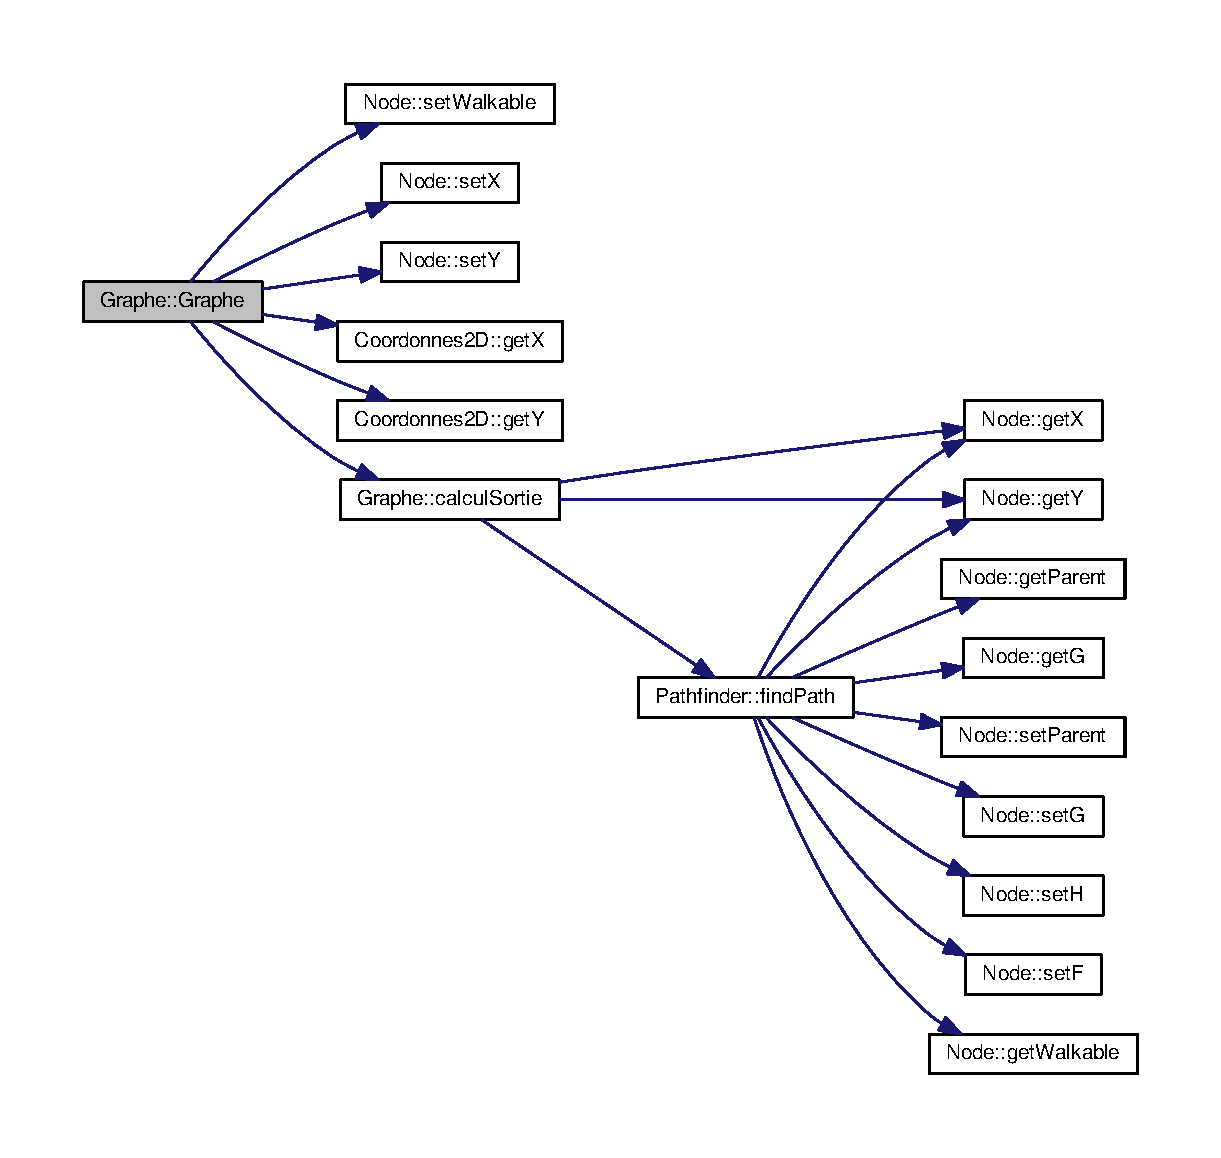
\includegraphics[width=350pt]{class_graphe_abd3e45f6d615a90d71106d29e6968c0f_cgraph}
\end{center}
\end{figure}


\index{Graphe@{Graphe}!$\sim$\-Graphe@{$\sim$\-Graphe}}
\index{$\sim$\-Graphe@{$\sim$\-Graphe}!Graphe@{Graphe}}
\subsubsection[{$\sim$\-Graphe}]{\setlength{\rightskip}{0pt plus 5cm}Graphe\-::$\sim$\-Graphe (
\begin{DoxyParamCaption}
{}
\end{DoxyParamCaption}
)\hspace{0.3cm}{\ttfamily [virtual]}}\label{class_graphe_a673c897db564767e9ace7169a5357310}


Destructeur. 

Destructeur de la classe \doxyref{Graphe}{p.}{class_graphe} 

\subsection{Documentation des fonctions membres}
\index{Graphe@{Graphe}!calcul\-Sortie@{calcul\-Sortie}}
\index{calcul\-Sortie@{calcul\-Sortie}!Graphe@{Graphe}}
\subsubsection[{calcul\-Sortie}]{\setlength{\rightskip}{0pt plus 5cm}std\-::vector$<$ {\bf Node} $\ast$ $>$ Graphe\-::calcul\-Sortie (
\begin{DoxyParamCaption}
\item[{std\-::vector$<$ {\bf Coordonnes2\-D} $>$ \&}]{sorties, }
\item[{{\bf Node} $\ast$}]{depart}
\end{DoxyParamCaption}
)}\label{class_graphe_a7c51dfd09bcf7d8505ec47a96b5d9c61}


Calcule la sortie la plus proche du point de depart. 


\begin{DoxyParams}{Paramètres}
{\em sorties} & \-: tableau contenant les coordonnees de toutes les sorties \\
\hline
{\em depart} & \-: \doxyref{Node}{p.}{class_node} de depart\\
\hline
\end{DoxyParams}
\begin{DoxyReturn}{Renvoie}
un chemin vers la sortie la plus proche de la position de depart 
\end{DoxyReturn}


Voici le graphe d'appel pour cette fonction \-:
\nopagebreak
\begin{figure}[H]
\begin{center}
\leavevmode
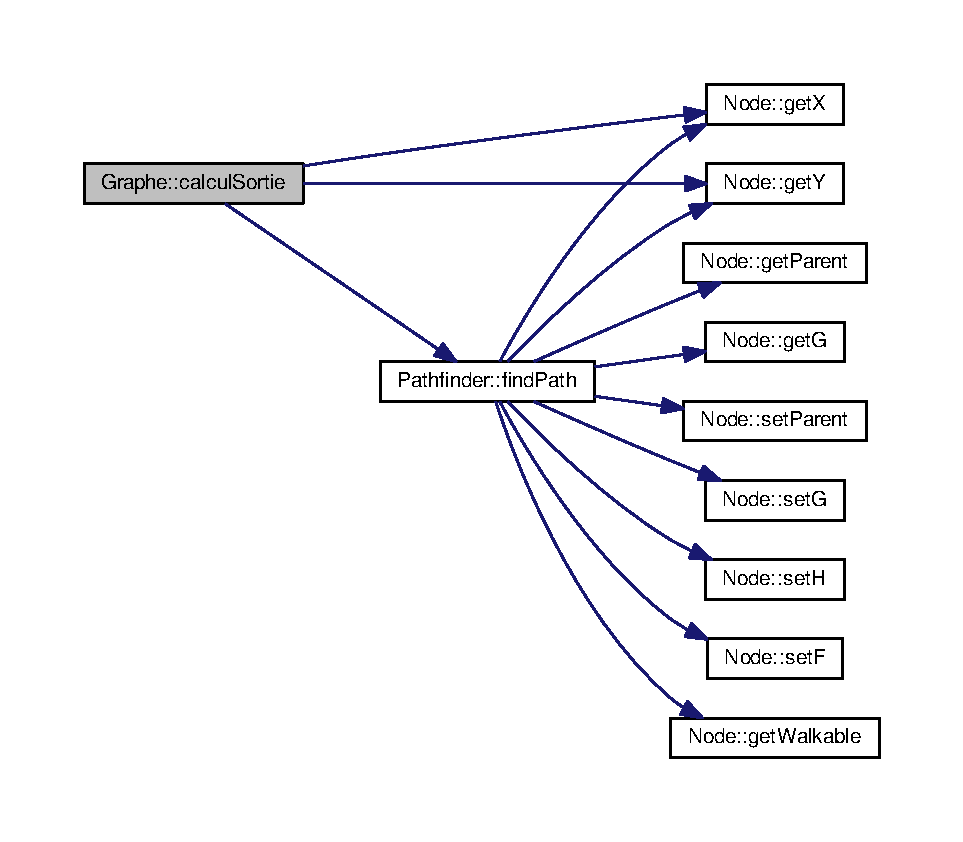
\includegraphics[width=350pt]{class_graphe_a7c51dfd09bcf7d8505ec47a96b5d9c61_cgraph}
\end{center}
\end{figure}




Voici le graphe des appelants de cette fonction \-:
\nopagebreak
\begin{figure}[H]
\begin{center}
\leavevmode
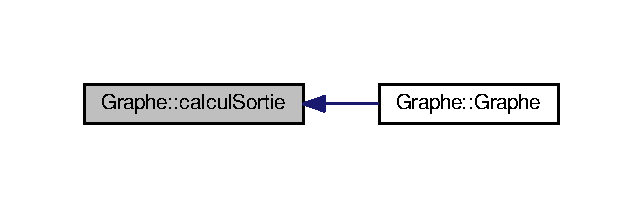
\includegraphics[width=308pt]{class_graphe_a7c51dfd09bcf7d8505ec47a96b5d9c61_icgraph}
\end{center}
\end{figure}


\index{Graphe@{Graphe}!get\-Chemin@{get\-Chemin}}
\index{get\-Chemin@{get\-Chemin}!Graphe@{Graphe}}
\subsubsection[{get\-Chemin}]{\setlength{\rightskip}{0pt plus 5cm}std\-::vector$<${\bf Node}$\ast$$>$ Graphe\-::get\-Chemin (
\begin{DoxyParamCaption}
{}
\end{DoxyParamCaption}
)\hspace{0.3cm}{\ttfamily [inline]}}\label{class_graphe_a6fae3a8286508021f0e040bc075e0c1d}


Getter de l'attribut m\-\_\-chemin de la classe \doxyref{Graphe}{p.}{class_graphe}. 

\begin{DoxyReturn}{Renvoie}
l'attribut m\-\_\-chemin de la classe \doxyref{Graphe}{p.}{class_graphe} 
\end{DoxyReturn}
\index{Graphe@{Graphe}!Nodes2\-Chemin\-X@{Nodes2\-Chemin\-X}}
\index{Nodes2\-Chemin\-X@{Nodes2\-Chemin\-X}!Graphe@{Graphe}}
\subsubsection[{Nodes2\-Chemin\-X}]{\setlength{\rightskip}{0pt plus 5cm}std\-::vector$<$ int $>$ Graphe\-::\-Nodes2\-Chemin\-X (
\begin{DoxyParamCaption}
\item[{std\-::vector$<$ {\bf Node} $\ast$ $>$}]{chemin}
\end{DoxyParamCaption}
)}\label{class_graphe_ac0e1b15961de7b45d61794b651654a66}


Conversion \doxyref{Node}{p.}{class_node} -\/$>$ Entiers (X) 

Convertie un tableau d'objets \doxyref{Node}{p.}{class_node} en tableau d'entier contenant les coordonnes X


\begin{DoxyParams}{Paramètres}
{\em chemin} & \-: tableau d'objets \doxyref{Node}{p.}{class_node} representant le chemin \\
\hline
\end{DoxyParams}
\begin{DoxyReturn}{Renvoie}
tableau d'entier contenant les coordonnes X du chemin 
\end{DoxyReturn}
\index{Graphe@{Graphe}!Nodes2\-Chemin\-Y@{Nodes2\-Chemin\-Y}}
\index{Nodes2\-Chemin\-Y@{Nodes2\-Chemin\-Y}!Graphe@{Graphe}}
\subsubsection[{Nodes2\-Chemin\-Y}]{\setlength{\rightskip}{0pt plus 5cm}std\-::vector$<$ int $>$ Graphe\-::\-Nodes2\-Chemin\-Y (
\begin{DoxyParamCaption}
\item[{std\-::vector$<$ {\bf Node} $\ast$ $>$}]{chemin}
\end{DoxyParamCaption}
)}\label{class_graphe_a3dc187933cfa37d917db230bd8b87db1}


Conversion \doxyref{Node}{p.}{class_node} -\/$>$ Entiers (Y) 

Convertie un tableau d'objets \doxyref{Node}{p.}{class_node} en tableau d'entier contenant les coordonnes Y


\begin{DoxyParams}{Paramètres}
{\em chemin} & \-: tableau d'objets \doxyref{Node}{p.}{class_node} representant le chemin \\
\hline
\end{DoxyParams}
\begin{DoxyReturn}{Renvoie}
tableau d'entier contenant les coordonnes Y du chemin 
\end{DoxyReturn}


La documentation de cette classe a été générée à partir des fichiers suivants \-:\begin{DoxyCompactItemize}
\item 
code/include/{\bf Graphe.\-h}\item 
code/src/Graphe.\-cpp\end{DoxyCompactItemize}

\section{Référence de la classe Humain}
\label{class_humain}\index{Humain@{Humain}}


classe representant un agent humain  




Graphe d'héritage de Humain\-:
\nopagebreak
\begin{figure}[H]
\begin{center}
\leavevmode
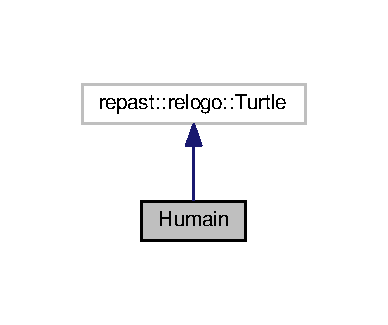
\includegraphics[width=186pt]{class_humain__inherit__graph}
\end{center}
\end{figure}


Graphe de collaboration de Humain\-:
\nopagebreak
\begin{figure}[H]
\begin{center}
\leavevmode
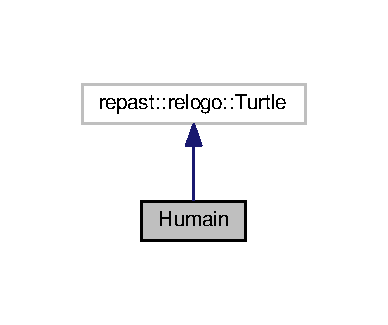
\includegraphics[width=186pt]{class_humain__coll__graph}
\end{center}
\end{figure}
\subsection*{Fonctions membres publiques}
\begin{DoxyCompactItemize}
\item 
{\bf Humain} (repast\-::\-Agent\-Id id, repast\-::relogo\-::\-Observer $\ast$obs)
\begin{DoxyCompactList}\small\item\em Constructeur. \end{DoxyCompactList}\item 
{\bf Humain} (repast\-::\-Agent\-Id id, repast\-::relogo\-::\-Observer $\ast$obs, const {\bf Agent\-Package} \&package)
\begin{DoxyCompactList}\small\item\em Constructeur pour le transfert d'agents. \end{DoxyCompactList}\item 
virtual {\bf $\sim$\-Humain} ()
\begin{DoxyCompactList}\small\item\em Destructeur. \end{DoxyCompactList}\item 
void {\bf get\-Pos} ()\label{class_humain_a6ef45c2a6398eee58bc985b0d3d04812}

\begin{DoxyCompactList}\small\item\em affiche la position d'un humain(coordonnees repast) \end{DoxyCompactList}\item 
void {\bf step} ()\label{class_humain_acfb526c278bfd003114e3f4270ab6342}

\begin{DoxyCompactList}\small\item\em fonction principale decrivant le comportement de l'agent (execute a chaque tick) \end{DoxyCompactList}\item 
void {\bf random\-Angle} (repast\-::\-Properties \&props)
\begin{DoxyCompactList}\small\item\em genere un angle aleatoire compris entre 0 et 359 (en degre) \end{DoxyCompactList}\item 
int {\bf random\-Type} (repast\-::\-Properties \&props)
\begin{DoxyCompactList}\small\item\em genere un type de personne aleatoire \end{DoxyCompactList}\item 
void {\bfseries afficher\-Pos} ({\bf Fenetre} $\ast$fen)\label{class_humain_aaef01ae3b778f16b1041f67c9c4a9424}

\item 
double {\bf get\-Angle} ()
\begin{DoxyCompactList}\small\item\em recupere l'angle actuel d'un agent \end{DoxyCompactList}\item 
double {\bf rad2deg} (double theta)
\begin{DoxyCompactList}\small\item\em conversion d'un angle de radians en degre \end{DoxyCompactList}\item 
double {\bf tourner\-Vers} (double x, double y)
\begin{DoxyCompactList}\small\item\em Calcule l'angle a prendre pour aller au point de coordonnees x/y. \end{DoxyCompactList}\item 
int {\bf get\-X\-Fichier} (void) const 
\begin{DoxyCompactList}\small\item\em Getter. \end{DoxyCompactList}\item 
int {\bf get\-Y\-Fichier} (void) const 
\begin{DoxyCompactList}\small\item\em Getter. \end{DoxyCompactList}\item 
int {\bf get\-X\-G\-L} (void) const 
\begin{DoxyCompactList}\small\item\em Getter. \end{DoxyCompactList}\item 
int {\bf get\-Y\-G\-L} (void) const 
\begin{DoxyCompactList}\small\item\em Getter. \end{DoxyCompactList}\item 
void {\bf set\-X\-Fichier} (int val)
\begin{DoxyCompactList}\small\item\em Setter. \end{DoxyCompactList}\item 
void {\bf set\-Y\-Fichier} (int val)
\begin{DoxyCompactList}\small\item\em Setter. \end{DoxyCompactList}\item 
void {\bf set\-X\-G\-L} (int val)
\begin{DoxyCompactList}\small\item\em Setter. \end{DoxyCompactList}\item 
void {\bf set\-Y\-G\-L} (int val)
\begin{DoxyCompactList}\small\item\em Setter. \end{DoxyCompactList}\item 
void {\bf set\-Angle} (double val)
\begin{DoxyCompactList}\small\item\em Setter. \end{DoxyCompactList}\item 
int {\bf get\-Type\-Personne} ()
\begin{DoxyCompactList}\small\item\em Getter. \end{DoxyCompactList}\item 
void {\bfseries set\-Type\-Personne} (int val)\label{class_humain_ade75c85dd706116d6bd20ef99da931ef}

\item 
int {\bf get\-Etape} ()
\begin{DoxyCompactList}\small\item\em Getter. \end{DoxyCompactList}\item 
bool {\bf get\-Sorti} ()
\begin{DoxyCompactList}\small\item\em Getter. \end{DoxyCompactList}\item 
std\-::vector$<$ int $>$ {\bf get\-Chemin\-X} ()
\begin{DoxyCompactList}\small\item\em Getter. \end{DoxyCompactList}\item 
std\-::vector$<$ int $>$ {\bf get\-Chemin\-Y} ()
\begin{DoxyCompactList}\small\item\em Getter. \end{DoxyCompactList}\item 
void {\bf set\-Chemin\-X\-Y} (std\-::vector$<$ int $>$ chemin\-X, std\-::vector$<$ int $>$ chemin\-Y, int etape, bool sorti)
\begin{DoxyCompactList}\small\item\em Setter. \end{DoxyCompactList}\end{DoxyCompactItemize}


\subsection{Description détaillée}
classe representant un agent humain 

La classe herite de la classe Turtle de repast, elle gere tout ce qui concerne le deplacement et l'orientation des humains, la communication entre humains, etc... 

\subsection{Documentation des constructeurs et destructeur}
\index{Humain@{Humain}!Humain@{Humain}}
\index{Humain@{Humain}!Humain@{Humain}}
\subsubsection[{Humain}]{\setlength{\rightskip}{0pt plus 5cm}Humain\-::\-Humain (
\begin{DoxyParamCaption}
\item[{repast\-::\-Agent\-Id}]{id, }
\item[{repast\-::relogo\-::\-Observer $\ast$}]{obs}
\end{DoxyParamCaption}
)\hspace{0.3cm}{\ttfamily [inline]}}\label{class_humain_a2ef84f203affc118025f145745323ddd}


Constructeur. 

Constructeur de la classe \doxyref{Humain}{p.}{class_humain}


\begin{DoxyParams}{Paramètres}
{\em id} & \-: Id de l'agent \\
\hline
{\em obs} & \-: pointeur vers l'Observer qui gere les agents \\
\hline
\end{DoxyParams}


Voici le graphe d'appel pour cette fonction \-:
\nopagebreak
\begin{figure}[H]
\begin{center}
\leavevmode
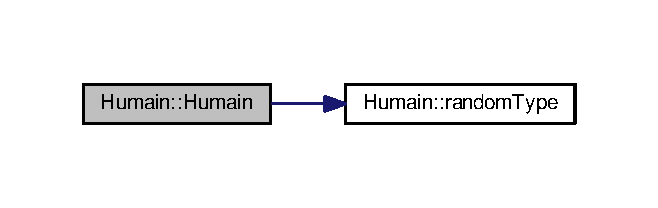
\includegraphics[width=316pt]{class_humain_a2ef84f203affc118025f145745323ddd_cgraph}
\end{center}
\end{figure}


\index{Humain@{Humain}!Humain@{Humain}}
\index{Humain@{Humain}!Humain@{Humain}}
\subsubsection[{Humain}]{\setlength{\rightskip}{0pt plus 5cm}Humain\-::\-Humain (
\begin{DoxyParamCaption}
\item[{repast\-::\-Agent\-Id}]{id, }
\item[{repast\-::relogo\-::\-Observer $\ast$}]{obs, }
\item[{const {\bf Agent\-Package} \&}]{package}
\end{DoxyParamCaption}
)\hspace{0.3cm}{\ttfamily [inline]}}\label{class_humain_a057f2b76521c2654a66dea6e9e2e33c5}


Constructeur pour le transfert d'agents. 

Constructeur de la classe \doxyref{Humain}{p.}{class_humain}


\begin{DoxyParams}{Paramètres}
{\em id} & \-: Id de l'agent \\
\hline
{\em obs} & \-: pointeur vers l'Observer qui gere les agents \\
\hline
{\em package} & \-: archive serialisee qui contient toutes les donnees necessaire pour creer un agent. \\
\hline
\end{DoxyParams}
\index{Humain@{Humain}!$\sim$\-Humain@{$\sim$\-Humain}}
\index{$\sim$\-Humain@{$\sim$\-Humain}!Humain@{Humain}}
\subsubsection[{$\sim$\-Humain}]{\setlength{\rightskip}{0pt plus 5cm}virtual Humain\-::$\sim$\-Humain (
\begin{DoxyParamCaption}
{}
\end{DoxyParamCaption}
)\hspace{0.3cm}{\ttfamily [inline]}, {\ttfamily [virtual]}}\label{class_humain_a08a0a8a77ce1877a76518e5d0acf03ca}


Destructeur. 

Destructeur de la classe \doxyref{Humain}{p.}{class_humain} 

\subsection{Documentation des fonctions membres}
\index{Humain@{Humain}!get\-Angle@{get\-Angle}}
\index{get\-Angle@{get\-Angle}!Humain@{Humain}}
\subsubsection[{get\-Angle}]{\setlength{\rightskip}{0pt plus 5cm}double Humain\-::get\-Angle (
\begin{DoxyParamCaption}
{}
\end{DoxyParamCaption}
)}\label{class_humain_a73d39a9d1f241d620ccac2f599e2dd97}


recupere l'angle actuel d'un agent 

\begin{DoxyReturn}{Renvoie}
l'angle de l'agent 
\end{DoxyReturn}


Voici le graphe des appelants de cette fonction \-:
\nopagebreak
\begin{figure}[H]
\begin{center}
\leavevmode
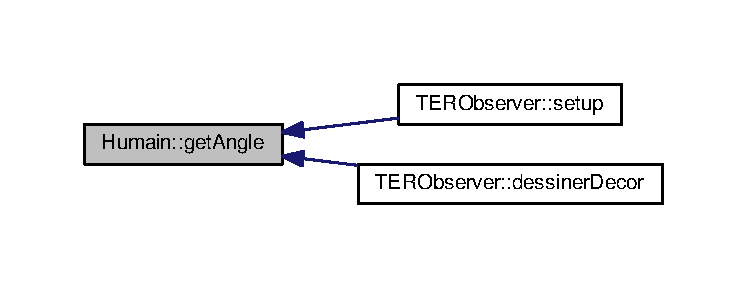
\includegraphics[width=350pt]{class_humain_a73d39a9d1f241d620ccac2f599e2dd97_icgraph}
\end{center}
\end{figure}


\index{Humain@{Humain}!get\-Chemin\-X@{get\-Chemin\-X}}
\index{get\-Chemin\-X@{get\-Chemin\-X}!Humain@{Humain}}
\subsubsection[{get\-Chemin\-X}]{\setlength{\rightskip}{0pt plus 5cm}std\-::vector$<$int$>$ Humain\-::get\-Chemin\-X (
\begin{DoxyParamCaption}
{}
\end{DoxyParamCaption}
)\hspace{0.3cm}{\ttfamily [inline]}}\label{class_humain_a68abc0ded73a07d369a74e5a4d3bd7e6}


Getter. 

\begin{DoxyReturn}{Renvoie}
l'attribut chemin\-X de la classe \doxyref{Humain}{p.}{class_humain} 
\end{DoxyReturn}


Voici le graphe des appelants de cette fonction \-:
\nopagebreak
\begin{figure}[H]
\begin{center}
\leavevmode
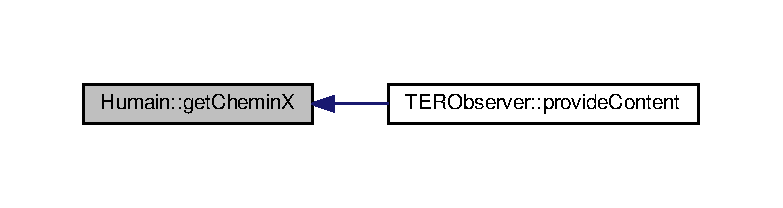
\includegraphics[width=350pt]{class_humain_a68abc0ded73a07d369a74e5a4d3bd7e6_icgraph}
\end{center}
\end{figure}


\index{Humain@{Humain}!get\-Chemin\-Y@{get\-Chemin\-Y}}
\index{get\-Chemin\-Y@{get\-Chemin\-Y}!Humain@{Humain}}
\subsubsection[{get\-Chemin\-Y}]{\setlength{\rightskip}{0pt plus 5cm}std\-::vector$<$int$>$ Humain\-::get\-Chemin\-Y (
\begin{DoxyParamCaption}
{}
\end{DoxyParamCaption}
)\hspace{0.3cm}{\ttfamily [inline]}}\label{class_humain_ad815b1e9aacefe7a41ded28772a41b9a}


Getter. 

\begin{DoxyReturn}{Renvoie}
l'attribut chemin\-Y de la classe \doxyref{Humain}{p.}{class_humain} 
\end{DoxyReturn}


Voici le graphe des appelants de cette fonction \-:
\nopagebreak
\begin{figure}[H]
\begin{center}
\leavevmode
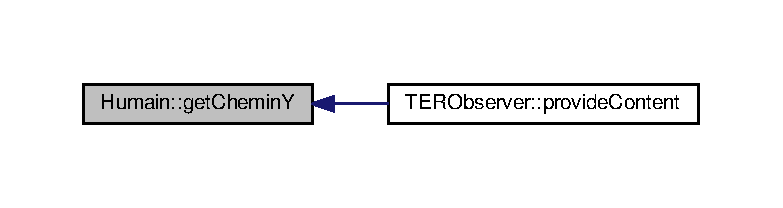
\includegraphics[width=350pt]{class_humain_ad815b1e9aacefe7a41ded28772a41b9a_icgraph}
\end{center}
\end{figure}


\index{Humain@{Humain}!get\-Etape@{get\-Etape}}
\index{get\-Etape@{get\-Etape}!Humain@{Humain}}
\subsubsection[{get\-Etape}]{\setlength{\rightskip}{0pt plus 5cm}int Humain\-::get\-Etape (
\begin{DoxyParamCaption}
{}
\end{DoxyParamCaption}
)\hspace{0.3cm}{\ttfamily [inline]}}\label{class_humain_a434d49c9e83f20f525106416f6c62a48}


Getter. 

\begin{DoxyReturn}{Renvoie}
l'attribut etape de la classe \doxyref{Humain}{p.}{class_humain} 
\end{DoxyReturn}


Voici le graphe des appelants de cette fonction \-:
\nopagebreak
\begin{figure}[H]
\begin{center}
\leavevmode
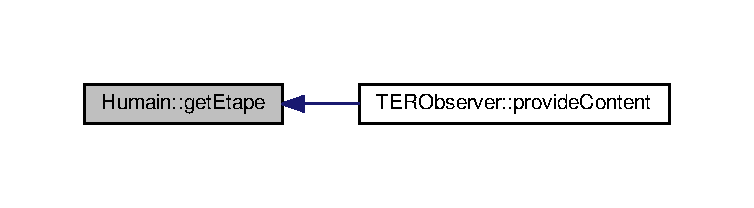
\includegraphics[width=350pt]{class_humain_a434d49c9e83f20f525106416f6c62a48_icgraph}
\end{center}
\end{figure}


\index{Humain@{Humain}!get\-Sorti@{get\-Sorti}}
\index{get\-Sorti@{get\-Sorti}!Humain@{Humain}}
\subsubsection[{get\-Sorti}]{\setlength{\rightskip}{0pt plus 5cm}bool Humain\-::get\-Sorti (
\begin{DoxyParamCaption}
{}
\end{DoxyParamCaption}
)\hspace{0.3cm}{\ttfamily [inline]}}\label{class_humain_a1351d4c106fc2e175cf19da0ca3fce52}


Getter. 

\begin{DoxyReturn}{Renvoie}
l'attribut sorti de la classe \doxyref{Humain}{p.}{class_humain} 
\end{DoxyReturn}


Voici le graphe des appelants de cette fonction \-:
\nopagebreak
\begin{figure}[H]
\begin{center}
\leavevmode
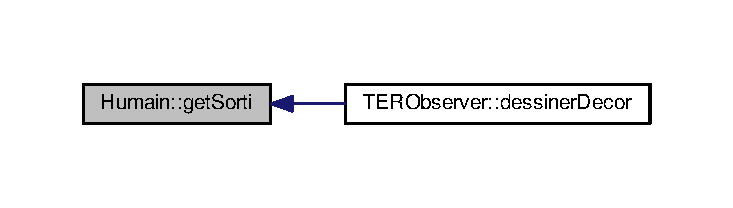
\includegraphics[width=350pt]{class_humain_a1351d4c106fc2e175cf19da0ca3fce52_icgraph}
\end{center}
\end{figure}


\index{Humain@{Humain}!get\-Type\-Personne@{get\-Type\-Personne}}
\index{get\-Type\-Personne@{get\-Type\-Personne}!Humain@{Humain}}
\subsubsection[{get\-Type\-Personne}]{\setlength{\rightskip}{0pt plus 5cm}int Humain\-::get\-Type\-Personne (
\begin{DoxyParamCaption}
{}
\end{DoxyParamCaption}
)\hspace{0.3cm}{\ttfamily [inline]}}\label{class_humain_ab8469bf829ed8100899bc57a62025cb9}


Getter. 

\begin{DoxyReturn}{Renvoie}
l'attribut type\-Personne de la classe \doxyref{Humain}{p.}{class_humain} 
\end{DoxyReturn}


Voici le graphe des appelants de cette fonction \-:
\nopagebreak
\begin{figure}[H]
\begin{center}
\leavevmode
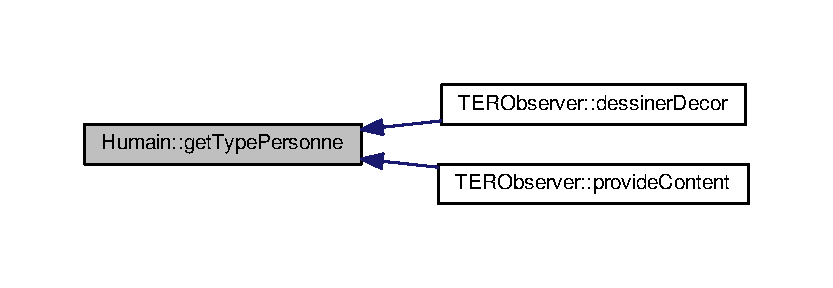
\includegraphics[width=350pt]{class_humain_ab8469bf829ed8100899bc57a62025cb9_icgraph}
\end{center}
\end{figure}


\index{Humain@{Humain}!get\-X\-Fichier@{get\-X\-Fichier}}
\index{get\-X\-Fichier@{get\-X\-Fichier}!Humain@{Humain}}
\subsubsection[{get\-X\-Fichier}]{\setlength{\rightskip}{0pt plus 5cm}int Humain\-::get\-X\-Fichier (
\begin{DoxyParamCaption}
\item[{void}]{}
\end{DoxyParamCaption}
) const\hspace{0.3cm}{\ttfamily [inline]}}\label{class_humain_a72f53748fcf1c862c46771208856a960}


Getter. 

\begin{DoxyReturn}{Renvoie}
l'attribut pos\-X\-Fichier de la classe \doxyref{Humain}{p.}{class_humain} 
\end{DoxyReturn}
\index{Humain@{Humain}!get\-X\-G\-L@{get\-X\-G\-L}}
\index{get\-X\-G\-L@{get\-X\-G\-L}!Humain@{Humain}}
\subsubsection[{get\-X\-G\-L}]{\setlength{\rightskip}{0pt plus 5cm}int Humain\-::get\-X\-G\-L (
\begin{DoxyParamCaption}
\item[{void}]{}
\end{DoxyParamCaption}
) const\hspace{0.3cm}{\ttfamily [inline]}}\label{class_humain_ad6179d5833fbc32eeb5cb440afdd58b0}


Getter. 

\begin{DoxyReturn}{Renvoie}
l'attribut pos\-X\-G\-L de la classe \doxyref{Humain}{p.}{class_humain} 
\end{DoxyReturn}
\index{Humain@{Humain}!get\-Y\-Fichier@{get\-Y\-Fichier}}
\index{get\-Y\-Fichier@{get\-Y\-Fichier}!Humain@{Humain}}
\subsubsection[{get\-Y\-Fichier}]{\setlength{\rightskip}{0pt plus 5cm}int Humain\-::get\-Y\-Fichier (
\begin{DoxyParamCaption}
\item[{void}]{}
\end{DoxyParamCaption}
) const\hspace{0.3cm}{\ttfamily [inline]}}\label{class_humain_a950ffa2b5fbfe59cdc5556598bb3fc36}


Getter. 

\begin{DoxyReturn}{Renvoie}
l'attribut pos\-Y\-Fichier de la classe \doxyref{Humain}{p.}{class_humain} 
\end{DoxyReturn}
\index{Humain@{Humain}!get\-Y\-G\-L@{get\-Y\-G\-L}}
\index{get\-Y\-G\-L@{get\-Y\-G\-L}!Humain@{Humain}}
\subsubsection[{get\-Y\-G\-L}]{\setlength{\rightskip}{0pt plus 5cm}int Humain\-::get\-Y\-G\-L (
\begin{DoxyParamCaption}
\item[{void}]{}
\end{DoxyParamCaption}
) const\hspace{0.3cm}{\ttfamily [inline]}}\label{class_humain_a476b49698c658f53675d8e2666990699}


Getter. 

\begin{DoxyReturn}{Renvoie}
l'attribut pos\-Y\-G\-L de la classe \doxyref{Humain}{p.}{class_humain} 
\end{DoxyReturn}
\index{Humain@{Humain}!rad2deg@{rad2deg}}
\index{rad2deg@{rad2deg}!Humain@{Humain}}
\subsubsection[{rad2deg}]{\setlength{\rightskip}{0pt plus 5cm}double Humain\-::rad2deg (
\begin{DoxyParamCaption}
\item[{double}]{theta}
\end{DoxyParamCaption}
)}\label{class_humain_a8987214bebd0063247cbfc1b4b5f1816}


conversion d'un angle de radians en degre 


\begin{DoxyParams}{Paramètres}
{\em theta} & \-: angle en radians\\
\hline
\end{DoxyParams}
\begin{DoxyReturn}{Renvoie}
angle en degre. 
\end{DoxyReturn}
\index{Humain@{Humain}!random\-Angle@{random\-Angle}}
\index{random\-Angle@{random\-Angle}!Humain@{Humain}}
\subsubsection[{random\-Angle}]{\setlength{\rightskip}{0pt plus 5cm}void Humain\-::random\-Angle (
\begin{DoxyParamCaption}
\item[{repast\-::\-Properties \&}]{props}
\end{DoxyParamCaption}
)}\label{class_humain_a415aa529a0f744d0b81bc80b93864665}


genere un angle aleatoire compris entre 0 et 359 (en degre) 


\begin{DoxyParams}{Paramètres}
{\em props} & \-: pointeur sur les proprietes de la simulation(pour le random seed) \\
\hline
\end{DoxyParams}


Voici le graphe des appelants de cette fonction \-:
\nopagebreak
\begin{figure}[H]
\begin{center}
\leavevmode
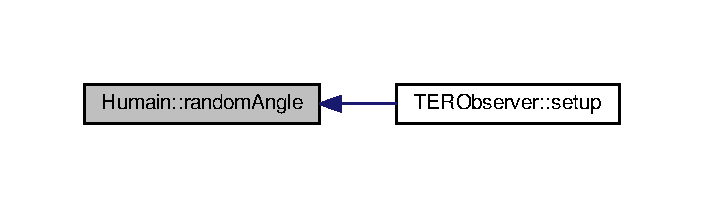
\includegraphics[width=338pt]{class_humain_a415aa529a0f744d0b81bc80b93864665_icgraph}
\end{center}
\end{figure}


\index{Humain@{Humain}!random\-Type@{random\-Type}}
\index{random\-Type@{random\-Type}!Humain@{Humain}}
\subsubsection[{random\-Type}]{\setlength{\rightskip}{0pt plus 5cm}int Humain\-::random\-Type (
\begin{DoxyParamCaption}
\item[{repast\-::\-Properties \&}]{props}
\end{DoxyParamCaption}
)}\label{class_humain_a0a9134ce08efbc5eb5714114de97fb63}


genere un type de personne aleatoire 


\begin{DoxyParams}{Paramètres}
{\em props} & \-: pointeur sur les proprietes de la simulation(pour le random seed)\\
\hline
\end{DoxyParams}
\begin{DoxyReturn}{Renvoie}
le typedepersonne genere. 
\end{DoxyReturn}


Voici le graphe des appelants de cette fonction \-:
\nopagebreak
\begin{figure}[H]
\begin{center}
\leavevmode
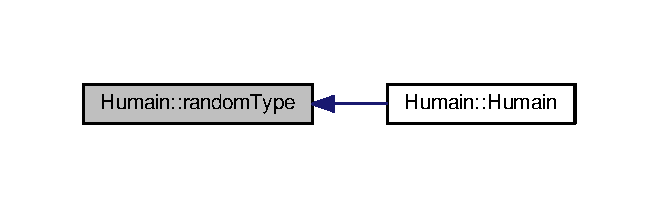
\includegraphics[width=316pt]{class_humain_a0a9134ce08efbc5eb5714114de97fb63_icgraph}
\end{center}
\end{figure}


\index{Humain@{Humain}!set\-Angle@{set\-Angle}}
\index{set\-Angle@{set\-Angle}!Humain@{Humain}}
\subsubsection[{set\-Angle}]{\setlength{\rightskip}{0pt plus 5cm}void Humain\-::set\-Angle (
\begin{DoxyParamCaption}
\item[{double}]{val}
\end{DoxyParamCaption}
)\hspace{0.3cm}{\ttfamily [inline]}}\label{class_humain_a2e50827e8e6c47f6671aae2bea409840}


Setter. 


\begin{DoxyParams}{Paramètres}
{\em val} & \-: nouvelle valeur pour l'attribut m\-\_\-angle de la classe \doxyref{Humain}{p.}{class_humain} \\
\hline
\end{DoxyParams}
\index{Humain@{Humain}!set\-Chemin\-X\-Y@{set\-Chemin\-X\-Y}}
\index{set\-Chemin\-X\-Y@{set\-Chemin\-X\-Y}!Humain@{Humain}}
\subsubsection[{set\-Chemin\-X\-Y}]{\setlength{\rightskip}{0pt plus 5cm}void Humain\-::set\-Chemin\-X\-Y (
\begin{DoxyParamCaption}
\item[{std\-::vector$<$ int $>$}]{chemin\-X, }
\item[{std\-::vector$<$ int $>$}]{chemin\-Y, }
\item[{int}]{etape, }
\item[{bool}]{sorti}
\end{DoxyParamCaption}
)\hspace{0.3cm}{\ttfamily [inline]}}\label{class_humain_a0dfad40c440229a41fb980af89385fc8}


Setter. 


\begin{DoxyParams}{Paramètres}
{\em chemin\-X} & \-: nouvelle valeur pour l'attribut chemin\-X de la classe \doxyref{Humain}{p.}{class_humain} \\
\hline
{\em chemin\-Y} & \-: nouvelle valeur pour l'attribut chemin\-Y de la classe \doxyref{Humain}{p.}{class_humain} \\
\hline
{\em etape} & \-: nouvelle valeur pour l'attribut etape de la classe \doxyref{Humain}{p.}{class_humain} \\
\hline
{\em sorti} & \-: nouvelle valeur pour l'attribut sorti de la classe \doxyref{Humain}{p.}{class_humain} \\
\hline
\end{DoxyParams}


Voici le graphe des appelants de cette fonction \-:
\nopagebreak
\begin{figure}[H]
\begin{center}
\leavevmode
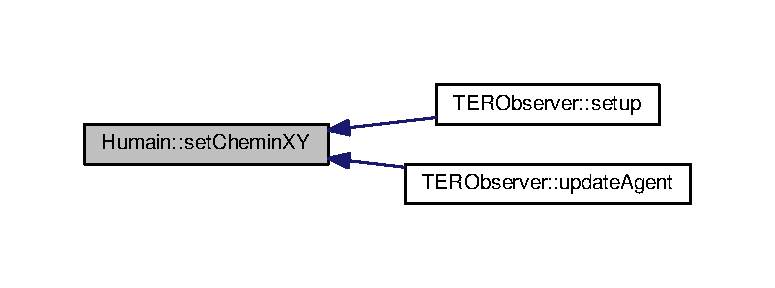
\includegraphics[width=350pt]{class_humain_a0dfad40c440229a41fb980af89385fc8_icgraph}
\end{center}
\end{figure}


\index{Humain@{Humain}!set\-X\-Fichier@{set\-X\-Fichier}}
\index{set\-X\-Fichier@{set\-X\-Fichier}!Humain@{Humain}}
\subsubsection[{set\-X\-Fichier}]{\setlength{\rightskip}{0pt plus 5cm}void Humain\-::set\-X\-Fichier (
\begin{DoxyParamCaption}
\item[{int}]{val}
\end{DoxyParamCaption}
)\hspace{0.3cm}{\ttfamily [inline]}}\label{class_humain_a8cc241895df70b2f6023552908903fab}


Setter. 


\begin{DoxyParams}{Paramètres}
{\em val} & \-: nouvelle valeur pour l'attribut pos\-X\-Fichier de la classe \doxyref{Humain}{p.}{class_humain} \\
\hline
\end{DoxyParams}
\index{Humain@{Humain}!set\-X\-G\-L@{set\-X\-G\-L}}
\index{set\-X\-G\-L@{set\-X\-G\-L}!Humain@{Humain}}
\subsubsection[{set\-X\-G\-L}]{\setlength{\rightskip}{0pt plus 5cm}void Humain\-::set\-X\-G\-L (
\begin{DoxyParamCaption}
\item[{int}]{val}
\end{DoxyParamCaption}
)\hspace{0.3cm}{\ttfamily [inline]}}\label{class_humain_aaa7d8c47d9f38e70454693ece8c78c81}


Setter. 


\begin{DoxyParams}{Paramètres}
{\em val} & \-: nouvelle valeur pour l'attribut pos\-X\-G\-L de la classe \doxyref{Humain}{p.}{class_humain} \\
\hline
\end{DoxyParams}
\index{Humain@{Humain}!set\-Y\-Fichier@{set\-Y\-Fichier}}
\index{set\-Y\-Fichier@{set\-Y\-Fichier}!Humain@{Humain}}
\subsubsection[{set\-Y\-Fichier}]{\setlength{\rightskip}{0pt plus 5cm}void Humain\-::set\-Y\-Fichier (
\begin{DoxyParamCaption}
\item[{int}]{val}
\end{DoxyParamCaption}
)\hspace{0.3cm}{\ttfamily [inline]}}\label{class_humain_a574c1d191014b8ce815b593b68422e54}


Setter. 


\begin{DoxyParams}{Paramètres}
{\em val} & \-: nouvelle valeur pour l'attribut pos\-Y\-Fichier de la classe \doxyref{Humain}{p.}{class_humain} \\
\hline
\end{DoxyParams}
\index{Humain@{Humain}!set\-Y\-G\-L@{set\-Y\-G\-L}}
\index{set\-Y\-G\-L@{set\-Y\-G\-L}!Humain@{Humain}}
\subsubsection[{set\-Y\-G\-L}]{\setlength{\rightskip}{0pt plus 5cm}void Humain\-::set\-Y\-G\-L (
\begin{DoxyParamCaption}
\item[{int}]{val}
\end{DoxyParamCaption}
)\hspace{0.3cm}{\ttfamily [inline]}}\label{class_humain_ab1ca792b176d3fb394f6aa411ba1e5f5}


Setter. 


\begin{DoxyParams}{Paramètres}
{\em val} & \-: nouvelle valeur pour l'attribut pos\-Y\-G\-L de la classe \doxyref{Humain}{p.}{class_humain} \\
\hline
\end{DoxyParams}
\index{Humain@{Humain}!tourner\-Vers@{tourner\-Vers}}
\index{tourner\-Vers@{tourner\-Vers}!Humain@{Humain}}
\subsubsection[{tourner\-Vers}]{\setlength{\rightskip}{0pt plus 5cm}double Humain\-::tourner\-Vers (
\begin{DoxyParamCaption}
\item[{double}]{x, }
\item[{double}]{y}
\end{DoxyParamCaption}
)}\label{class_humain_ad7777f2198c8f306bfc8040afe7f0802}


Calcule l'angle a prendre pour aller au point de coordonnees x/y. 


\begin{DoxyParams}{Paramètres}
{\em x} & \-: coordonne x de l'emplacement ou on veut aller \\
\hline
{\em y} & \-: coordonne y de l'emplacement ou on veut aller \\
\hline
\end{DoxyParams}
\begin{DoxyReturn}{Renvoie}
angle vers le point de destination. 
\end{DoxyReturn}


La documentation de cette classe a été générée à partir des fichiers suivants \-:\begin{DoxyCompactItemize}
\item 
code/include/{\bf Humain.\-h}\item 
code/src/Humain.\-cpp\end{DoxyCompactItemize}

\section{Référence de la classe Mur}
\label{class_mur}\index{Mur@{Mur}}


Classe representant un \doxyref{Mur}{p.}{class_mur}.  




{\ttfamily \#include $<$Mur.\-h$>$}



Graphe d'héritage de Mur\-:
\nopagebreak
\begin{figure}[H]
\begin{center}
\leavevmode
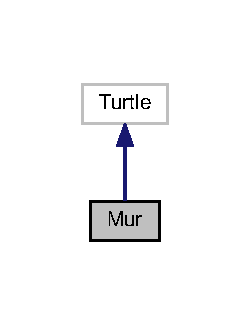
\includegraphics[width=120pt]{class_mur__inherit__graph}
\end{center}
\end{figure}


Graphe de collaboration de Mur\-:
\nopagebreak
\begin{figure}[H]
\begin{center}
\leavevmode
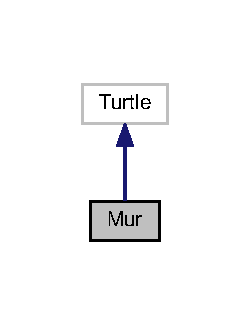
\includegraphics[width=120pt]{class_mur__coll__graph}
\end{center}
\end{figure}
\subsection*{Fonctions membres publiques}
\begin{DoxyCompactItemize}
\item 
{\bf Mur} (repast\-::\-Agent\-Id id, repast\-::relogo\-::\-Observer $\ast$obs)
\begin{DoxyCompactList}\small\item\em Constructeur. \end{DoxyCompactList}\item 
{\bf Mur} (repast\-::\-Agent\-Id id, repast\-::relogo\-::\-Observer $\ast$obs, const {\bf Agent\-Package} \&package)
\begin{DoxyCompactList}\small\item\em Constructeur pour le transfert d'agents (ici inutile car les murs ne se deplacent pas) \end{DoxyCompactList}\item 
virtual {\bf $\sim$\-Mur} ()
\begin{DoxyCompactList}\small\item\em Destructeur. \end{DoxyCompactList}\end{DoxyCompactItemize}


\subsection{Description détaillée}
Classe representant un \doxyref{Mur}{p.}{class_mur}. 

\subsection{Documentation des constructeurs et destructeur}
\index{Mur@{Mur}!Mur@{Mur}}
\index{Mur@{Mur}!Mur@{Mur}}
\subsubsection[{Mur}]{\setlength{\rightskip}{0pt plus 5cm}Mur\-::\-Mur (
\begin{DoxyParamCaption}
\item[{repast\-::\-Agent\-Id}]{id, }
\item[{repast\-::relogo\-::\-Observer $\ast$}]{obs}
\end{DoxyParamCaption}
)\hspace{0.3cm}{\ttfamily [inline]}}\label{class_mur_a82c0c9f5f75453e37c2972aae0f93eb4}


Constructeur. 

Constructeur de la classe \doxyref{Mur}{p.}{class_mur}


\begin{DoxyParams}{Paramètres}
{\em id} & \-: Id de l'agent \\
\hline
{\em obs} & \-: pointeur vers l'Observer qui gere les agents \\
\hline
\end{DoxyParams}
\index{Mur@{Mur}!Mur@{Mur}}
\index{Mur@{Mur}!Mur@{Mur}}
\subsubsection[{Mur}]{\setlength{\rightskip}{0pt plus 5cm}Mur\-::\-Mur (
\begin{DoxyParamCaption}
\item[{repast\-::\-Agent\-Id}]{id, }
\item[{repast\-::relogo\-::\-Observer $\ast$}]{obs, }
\item[{const {\bf Agent\-Package} \&}]{package}
\end{DoxyParamCaption}
)\hspace{0.3cm}{\ttfamily [inline]}}\label{class_mur_a3e715ac0818a44458fa461287dd73796}


Constructeur pour le transfert d'agents (ici inutile car les murs ne se deplacent pas) 

Constructeur de la classe \doxyref{Mur}{p.}{class_mur}


\begin{DoxyParams}{Paramètres}
{\em id} & \-: Id de l'agent \\
\hline
{\em obs} & \-: pointeur vers l'Observer qui gere les agents \\
\hline
{\em package} & \-: archive serialisee qui contient toutes les donnees necessaire pour creer un agent. \\
\hline
\end{DoxyParams}
\index{Mur@{Mur}!$\sim$\-Mur@{$\sim$\-Mur}}
\index{$\sim$\-Mur@{$\sim$\-Mur}!Mur@{Mur}}
\subsubsection[{$\sim$\-Mur}]{\setlength{\rightskip}{0pt plus 5cm}virtual Mur\-::$\sim$\-Mur (
\begin{DoxyParamCaption}
{}
\end{DoxyParamCaption}
)\hspace{0.3cm}{\ttfamily [inline]}, {\ttfamily [virtual]}}\label{class_mur_aa5655c3522b0a40f520666f7ca895f3d}


Destructeur. 

Destructeur de la classe \doxyref{Humain}{p.}{class_humain} 

La documentation de cette classe a été générée à partir du fichier suivant \-:\begin{DoxyCompactItemize}
\item 
code/include/{\bf Mur.\-h}\end{DoxyCompactItemize}

\section{Référence de la classe Node}
\label{class_node}\index{Node@{Node}}


Classe representant un \doxyref{Node}{p.}{class_node} Un \doxyref{Node}{p.}{class_node} est une \char`\"{}case\char`\"{} de la matrice representant le monde Repast, chaque node contient les heuristiques,g,h et f, une position X et Y , un \doxyref{Node}{p.}{class_node} Parent, et un boolean indiquant si le node est un mur ou pas.  




{\ttfamily \#include $<$Node.\-h$>$}

\subsection*{Fonctions membres publiques}
\begin{DoxyCompactItemize}
\item 
{\bf Node} ()
\begin{DoxyCompactList}\small\item\em Constructeur. \end{DoxyCompactList}\item 
virtual {\bf $\sim$\-Node} ()
\begin{DoxyCompactList}\small\item\em Destructeur. \end{DoxyCompactList}\item 
bool {\bf est\-Egal} ({\bf Node} const \&b) const 
\begin{DoxyCompactList}\small\item\em Compare deux objets de type \doxyref{Node}{p.}{class_node}. \end{DoxyCompactList}\item 
void {\bf set\-Parent} ({\bf Node} $\ast$val)
\begin{DoxyCompactList}\small\item\em Setter de l'attribut Parent de la classe \doxyref{Node}{p.}{class_node}. \end{DoxyCompactList}\item 
{\bf Node} $\ast$ {\bf get\-Parent} ()
\begin{DoxyCompactList}\small\item\em Getter de l'attribut m\-\_\-parent de la classe \doxyref{Node}{p.}{class_node}. \end{DoxyCompactList}\item 
void {\bf set\-Walkable} (bool val)
\begin{DoxyCompactList}\small\item\em Setter de l'attribut m\-\_\-walkable de la classe \doxyref{Node}{p.}{class_node}. \end{DoxyCompactList}\item 
void {\bf set\-G} (int val)
\begin{DoxyCompactList}\small\item\em Setter de l'attribut m\-\_\-\-G de la classe \doxyref{Node}{p.}{class_node}. \end{DoxyCompactList}\item 
void {\bf set\-F} (int val)
\begin{DoxyCompactList}\small\item\em Setter de l'attribut m\-\_\-\-F de la classe \doxyref{Node}{p.}{class_node}. \end{DoxyCompactList}\item 
void {\bf set\-H} (int val)
\begin{DoxyCompactList}\small\item\em Setter de l'attribut m\-\_\-h de la classe \doxyref{Node}{p.}{class_node}. \end{DoxyCompactList}\item 
void {\bf set\-X} (int val)
\begin{DoxyCompactList}\small\item\em Setter de l'attribut m\-\_\-\-X de la classe \doxyref{Node}{p.}{class_node}. \end{DoxyCompactList}\item 
void {\bf set\-Y} (int val)
\begin{DoxyCompactList}\small\item\em Setter de l'attribut m\-\_\-\-Y de la classe \doxyref{Node}{p.}{class_node}. \end{DoxyCompactList}\item 
bool {\bf get\-Walkable} ()
\begin{DoxyCompactList}\small\item\em Getter de l'attribut m\-\_\-walkable de la classe \doxyref{Node}{p.}{class_node}. \end{DoxyCompactList}\item 
int {\bf get\-G} ()
\begin{DoxyCompactList}\small\item\em Getter de l'attribut m\-\_\-\-G de la classe \doxyref{Node}{p.}{class_node}. \end{DoxyCompactList}\item 
int {\bf get\-F} ()
\begin{DoxyCompactList}\small\item\em Getter de l'attribut m\-\_\-\-F de la classe \doxyref{Node}{p.}{class_node}. \end{DoxyCompactList}\item 
int {\bf get\-H} ()
\begin{DoxyCompactList}\small\item\em Getter de l'attribut m\-\_\-\-H de la classe \doxyref{Node}{p.}{class_node}. \end{DoxyCompactList}\item 
int {\bf get\-X} ()
\begin{DoxyCompactList}\small\item\em Getter de l'attribut m\-\_\-\-X de la classe \doxyref{Node}{p.}{class_node}. \end{DoxyCompactList}\item 
int {\bf get\-Y} ()
\begin{DoxyCompactList}\small\item\em Getter de l'attribut m\-\_\-\-Y de la classe \doxyref{Node}{p.}{class_node}. \end{DoxyCompactList}\end{DoxyCompactItemize}


\subsection{Description détaillée}
Classe representant un \doxyref{Node}{p.}{class_node} Un \doxyref{Node}{p.}{class_node} est une \char`\"{}case\char`\"{} de la matrice representant le monde Repast, chaque node contient les heuristiques,g,h et f, une position X et Y , un \doxyref{Node}{p.}{class_node} Parent, et un boolean indiquant si le node est un mur ou pas. 

\subsection{Documentation des constructeurs et destructeur}
\index{Node@{Node}!Node@{Node}}
\index{Node@{Node}!Node@{Node}}
\subsubsection[{Node}]{\setlength{\rightskip}{0pt plus 5cm}Node\-::\-Node (
\begin{DoxyParamCaption}
{}
\end{DoxyParamCaption}
)}\label{class_node_ad7a34779cad45d997bfd6d3d8043c75f}


Constructeur. 

Constructeur de la classe \doxyref{Node}{p.}{class_node} \index{Node@{Node}!$\sim$\-Node@{$\sim$\-Node}}
\index{$\sim$\-Node@{$\sim$\-Node}!Node@{Node}}
\subsubsection[{$\sim$\-Node}]{\setlength{\rightskip}{0pt plus 5cm}Node\-::$\sim$\-Node (
\begin{DoxyParamCaption}
{}
\end{DoxyParamCaption}
)\hspace{0.3cm}{\ttfamily [virtual]}}\label{class_node_aa0840c3cb5c7159be6d992adecd2097c}


Destructeur. 

Destructeur de la classe \doxyref{Node}{p.}{class_node} 

\subsection{Documentation des fonctions membres}
\index{Node@{Node}!est\-Egal@{est\-Egal}}
\index{est\-Egal@{est\-Egal}!Node@{Node}}
\subsubsection[{est\-Egal}]{\setlength{\rightskip}{0pt plus 5cm}bool Node\-::est\-Egal (
\begin{DoxyParamCaption}
\item[{{\bf Node} const \&}]{b}
\end{DoxyParamCaption}
) const}\label{class_node_aa342abc3125e21fab6c9085aefb9f90f}


Compare deux objets de type \doxyref{Node}{p.}{class_node}. 


\begin{DoxyParams}{Paramètres}
{\em b} & \-: node a comparer au \doxyref{Node}{p.}{class_node} actuel \\
\hline
\end{DoxyParams}
\begin{DoxyReturn}{Renvoie}
un boolean idiquant si les deux nodes sont egaux. 
\end{DoxyReturn}
\index{Node@{Node}!get\-F@{get\-F}}
\index{get\-F@{get\-F}!Node@{Node}}
\subsubsection[{get\-F}]{\setlength{\rightskip}{0pt plus 5cm}int Node\-::get\-F (
\begin{DoxyParamCaption}
{}
\end{DoxyParamCaption}
)\hspace{0.3cm}{\ttfamily [inline]}}\label{class_node_a7b012d2404cc65fb58a9bb3a2dc6d724}


Getter de l'attribut m\-\_\-\-F de la classe \doxyref{Node}{p.}{class_node}. 

\begin{DoxyReturn}{Renvoie}
valeur de l'attribut m\-\_\-\-F de la classe \doxyref{Node}{p.}{class_node} 
\end{DoxyReturn}
\index{Node@{Node}!get\-G@{get\-G}}
\index{get\-G@{get\-G}!Node@{Node}}
\subsubsection[{get\-G}]{\setlength{\rightskip}{0pt plus 5cm}int Node\-::get\-G (
\begin{DoxyParamCaption}
{}
\end{DoxyParamCaption}
)\hspace{0.3cm}{\ttfamily [inline]}}\label{class_node_a9133c5c2e1c994b914535bbbefa33d7c}


Getter de l'attribut m\-\_\-\-G de la classe \doxyref{Node}{p.}{class_node}. 

\begin{DoxyReturn}{Renvoie}
valeur de l'attribut m\-\_\-\-G de la classe \doxyref{Node}{p.}{class_node} 
\end{DoxyReturn}


Voici le graphe des appelants de cette fonction \-:
\nopagebreak
\begin{figure}[H]
\begin{center}
\leavevmode
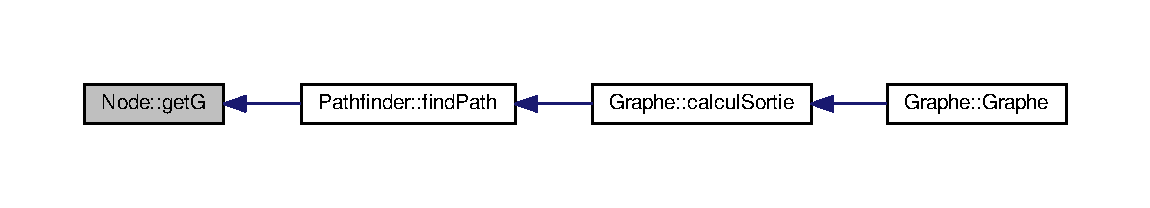
\includegraphics[width=350pt]{class_node_a9133c5c2e1c994b914535bbbefa33d7c_icgraph}
\end{center}
\end{figure}


\index{Node@{Node}!get\-H@{get\-H}}
\index{get\-H@{get\-H}!Node@{Node}}
\subsubsection[{get\-H}]{\setlength{\rightskip}{0pt plus 5cm}int Node\-::get\-H (
\begin{DoxyParamCaption}
{}
\end{DoxyParamCaption}
)\hspace{0.3cm}{\ttfamily [inline]}}\label{class_node_a1108111505a673b217d5e13d6ac36d14}


Getter de l'attribut m\-\_\-\-H de la classe \doxyref{Node}{p.}{class_node}. 

\begin{DoxyReturn}{Renvoie}
valeur de l'attribut m\-\_\-\-H de la classe \doxyref{Node}{p.}{class_node} 
\end{DoxyReturn}
\index{Node@{Node}!get\-Parent@{get\-Parent}}
\index{get\-Parent@{get\-Parent}!Node@{Node}}
\subsubsection[{get\-Parent}]{\setlength{\rightskip}{0pt plus 5cm}{\bf Node} $\ast$ Node\-::get\-Parent (
\begin{DoxyParamCaption}
{}
\end{DoxyParamCaption}
)}\label{class_node_a220a8d64cb0df1cce083ed38c1260615}


Getter de l'attribut m\-\_\-parent de la classe \doxyref{Node}{p.}{class_node}. 

\begin{DoxyReturn}{Renvoie}
valeur de l'attribut m\-\_\-parent de la classe \doxyref{Node}{p.}{class_node} 
\end{DoxyReturn}


Voici le graphe des appelants de cette fonction \-:
\nopagebreak
\begin{figure}[H]
\begin{center}
\leavevmode
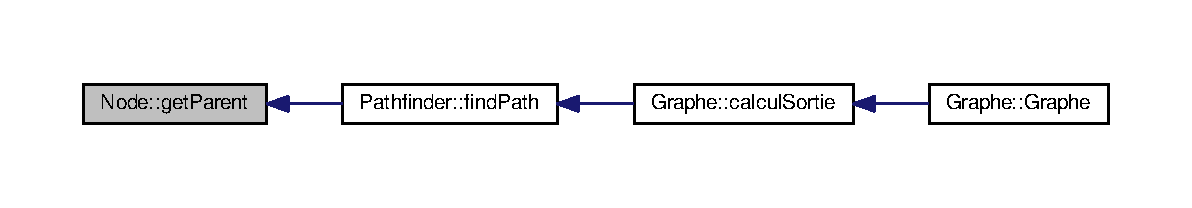
\includegraphics[width=350pt]{class_node_a220a8d64cb0df1cce083ed38c1260615_icgraph}
\end{center}
\end{figure}


\index{Node@{Node}!get\-Walkable@{get\-Walkable}}
\index{get\-Walkable@{get\-Walkable}!Node@{Node}}
\subsubsection[{get\-Walkable}]{\setlength{\rightskip}{0pt plus 5cm}bool Node\-::get\-Walkable (
\begin{DoxyParamCaption}
{}
\end{DoxyParamCaption}
)\hspace{0.3cm}{\ttfamily [inline]}}\label{class_node_af04dc1e91f0961108c3ffab1fc9e792a}


Getter de l'attribut m\-\_\-walkable de la classe \doxyref{Node}{p.}{class_node}. 

\begin{DoxyReturn}{Renvoie}
valeur de l'attribut m\-\_\-walkable de la classe \doxyref{Node}{p.}{class_node} 
\end{DoxyReturn}


Voici le graphe des appelants de cette fonction \-:
\nopagebreak
\begin{figure}[H]
\begin{center}
\leavevmode
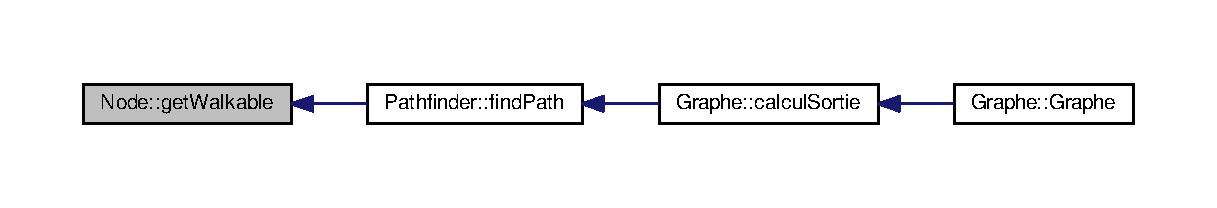
\includegraphics[width=350pt]{class_node_af04dc1e91f0961108c3ffab1fc9e792a_icgraph}
\end{center}
\end{figure}


\index{Node@{Node}!get\-X@{get\-X}}
\index{get\-X@{get\-X}!Node@{Node}}
\subsubsection[{get\-X}]{\setlength{\rightskip}{0pt plus 5cm}int Node\-::get\-X (
\begin{DoxyParamCaption}
{}
\end{DoxyParamCaption}
)\hspace{0.3cm}{\ttfamily [inline]}}\label{class_node_a6c026e5d8c28591c6e2bd08c68619fd1}


Getter de l'attribut m\-\_\-\-X de la classe \doxyref{Node}{p.}{class_node}. 

\begin{DoxyReturn}{Renvoie}
valeur de l'attribut m\-\_\-\-X de la classe \doxyref{Node}{p.}{class_node} 
\end{DoxyReturn}


Voici le graphe des appelants de cette fonction \-:
\nopagebreak
\begin{figure}[H]
\begin{center}
\leavevmode
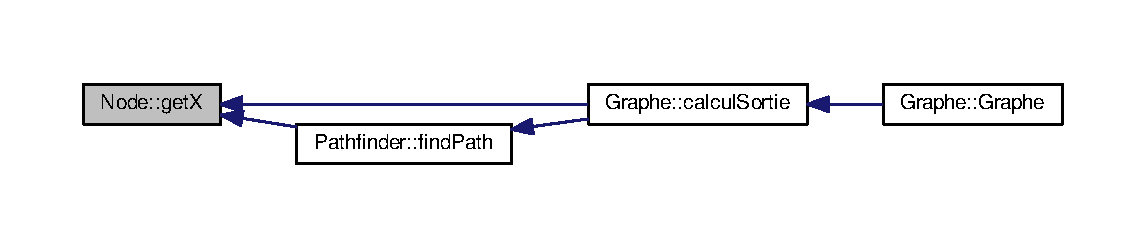
\includegraphics[width=350pt]{class_node_a6c026e5d8c28591c6e2bd08c68619fd1_icgraph}
\end{center}
\end{figure}


\index{Node@{Node}!get\-Y@{get\-Y}}
\index{get\-Y@{get\-Y}!Node@{Node}}
\subsubsection[{get\-Y}]{\setlength{\rightskip}{0pt plus 5cm}int Node\-::get\-Y (
\begin{DoxyParamCaption}
{}
\end{DoxyParamCaption}
)\hspace{0.3cm}{\ttfamily [inline]}}\label{class_node_abab48a3f494994d4f456897f3372d3ae}


Getter de l'attribut m\-\_\-\-Y de la classe \doxyref{Node}{p.}{class_node}. 

\begin{DoxyReturn}{Renvoie}
valeur de l'attribut m\-\_\-\-Y de la classe \doxyref{Node}{p.}{class_node} 
\end{DoxyReturn}


Voici le graphe des appelants de cette fonction \-:
\nopagebreak
\begin{figure}[H]
\begin{center}
\leavevmode
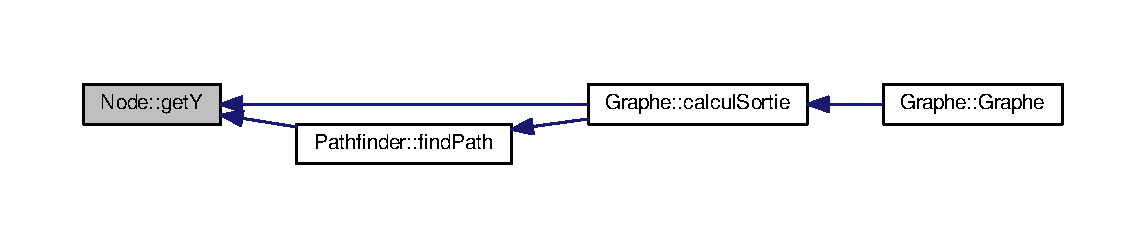
\includegraphics[width=350pt]{class_node_abab48a3f494994d4f456897f3372d3ae_icgraph}
\end{center}
\end{figure}


\index{Node@{Node}!set\-F@{set\-F}}
\index{set\-F@{set\-F}!Node@{Node}}
\subsubsection[{set\-F}]{\setlength{\rightskip}{0pt plus 5cm}void Node\-::set\-F (
\begin{DoxyParamCaption}
\item[{int}]{val}
\end{DoxyParamCaption}
)\hspace{0.3cm}{\ttfamily [inline]}}\label{class_node_a070cae6ce68d13a77b42686e6ecdef05}


Setter de l'attribut m\-\_\-\-F de la classe \doxyref{Node}{p.}{class_node}. 


\begin{DoxyParams}{Paramètres}
{\em val} & \-: valeur de l'attribut a modifier \\
\hline
\end{DoxyParams}


Voici le graphe des appelants de cette fonction \-:
\nopagebreak
\begin{figure}[H]
\begin{center}
\leavevmode
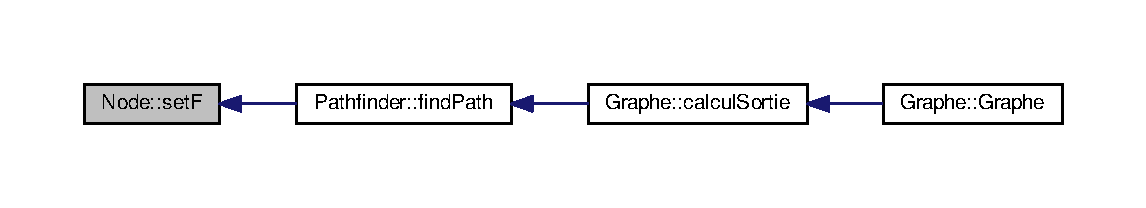
\includegraphics[width=350pt]{class_node_a070cae6ce68d13a77b42686e6ecdef05_icgraph}
\end{center}
\end{figure}


\index{Node@{Node}!set\-G@{set\-G}}
\index{set\-G@{set\-G}!Node@{Node}}
\subsubsection[{set\-G}]{\setlength{\rightskip}{0pt plus 5cm}void Node\-::set\-G (
\begin{DoxyParamCaption}
\item[{int}]{val}
\end{DoxyParamCaption}
)\hspace{0.3cm}{\ttfamily [inline]}}\label{class_node_a47181f2860b050a0036097d534051cfc}


Setter de l'attribut m\-\_\-\-G de la classe \doxyref{Node}{p.}{class_node}. 


\begin{DoxyParams}{Paramètres}
{\em val} & \-: valeur de l'attribut a modifier \\
\hline
\end{DoxyParams}


Voici le graphe des appelants de cette fonction \-:
\nopagebreak
\begin{figure}[H]
\begin{center}
\leavevmode
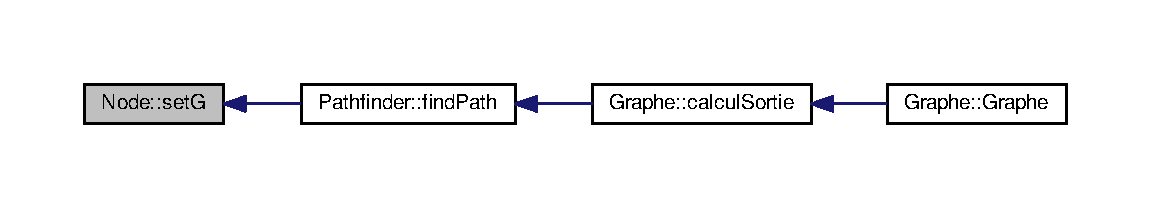
\includegraphics[width=350pt]{class_node_a47181f2860b050a0036097d534051cfc_icgraph}
\end{center}
\end{figure}


\index{Node@{Node}!set\-H@{set\-H}}
\index{set\-H@{set\-H}!Node@{Node}}
\subsubsection[{set\-H}]{\setlength{\rightskip}{0pt plus 5cm}void Node\-::set\-H (
\begin{DoxyParamCaption}
\item[{int}]{val}
\end{DoxyParamCaption}
)\hspace{0.3cm}{\ttfamily [inline]}}\label{class_node_a5f9637d2e5bed720d9ee7a5af8a00c36}


Setter de l'attribut m\-\_\-h de la classe \doxyref{Node}{p.}{class_node}. 


\begin{DoxyParams}{Paramètres}
{\em val} & \-: valeur de l'attribut a modifier \\
\hline
\end{DoxyParams}


Voici le graphe des appelants de cette fonction \-:
\nopagebreak
\begin{figure}[H]
\begin{center}
\leavevmode
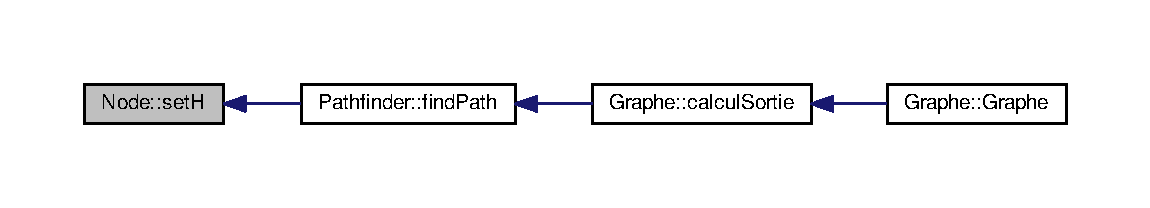
\includegraphics[width=350pt]{class_node_a5f9637d2e5bed720d9ee7a5af8a00c36_icgraph}
\end{center}
\end{figure}


\index{Node@{Node}!set\-Parent@{set\-Parent}}
\index{set\-Parent@{set\-Parent}!Node@{Node}}
\subsubsection[{set\-Parent}]{\setlength{\rightskip}{0pt plus 5cm}void Node\-::set\-Parent (
\begin{DoxyParamCaption}
\item[{{\bf Node} $\ast$}]{val}
\end{DoxyParamCaption}
)}\label{class_node_a39cc5b0b6814a6a2f4f0771203f334a1}


Setter de l'attribut Parent de la classe \doxyref{Node}{p.}{class_node}. 


\begin{DoxyParams}{Paramètres}
{\em val} & \-: valeur de l'attribut a modifier \\
\hline
\end{DoxyParams}


Voici le graphe des appelants de cette fonction \-:
\nopagebreak
\begin{figure}[H]
\begin{center}
\leavevmode
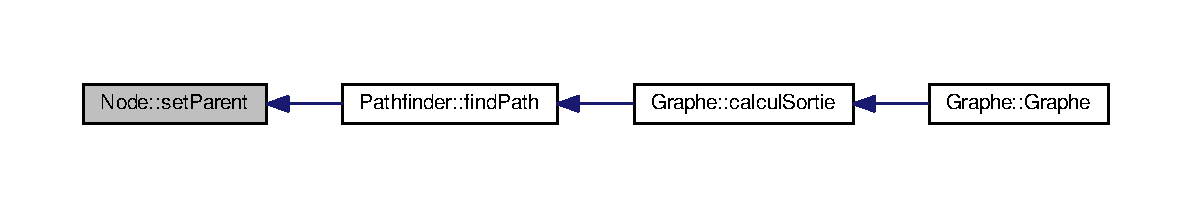
\includegraphics[width=350pt]{class_node_a39cc5b0b6814a6a2f4f0771203f334a1_icgraph}
\end{center}
\end{figure}


\index{Node@{Node}!set\-Walkable@{set\-Walkable}}
\index{set\-Walkable@{set\-Walkable}!Node@{Node}}
\subsubsection[{set\-Walkable}]{\setlength{\rightskip}{0pt plus 5cm}void Node\-::set\-Walkable (
\begin{DoxyParamCaption}
\item[{bool}]{val}
\end{DoxyParamCaption}
)\hspace{0.3cm}{\ttfamily [inline]}}\label{class_node_a281acda069a341e04b5e9dbd45c4658e}


Setter de l'attribut m\-\_\-walkable de la classe \doxyref{Node}{p.}{class_node}. 


\begin{DoxyParams}{Paramètres}
{\em val} & \-: valeur de l'attribut a modifier \\
\hline
\end{DoxyParams}


Voici le graphe des appelants de cette fonction \-:
\nopagebreak
\begin{figure}[H]
\begin{center}
\leavevmode
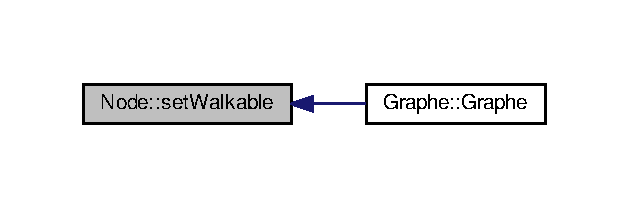
\includegraphics[width=302pt]{class_node_a281acda069a341e04b5e9dbd45c4658e_icgraph}
\end{center}
\end{figure}


\index{Node@{Node}!set\-X@{set\-X}}
\index{set\-X@{set\-X}!Node@{Node}}
\subsubsection[{set\-X}]{\setlength{\rightskip}{0pt plus 5cm}void Node\-::set\-X (
\begin{DoxyParamCaption}
\item[{int}]{val}
\end{DoxyParamCaption}
)\hspace{0.3cm}{\ttfamily [inline]}}\label{class_node_accabc02cdc5144636cab8d5079619d13}


Setter de l'attribut m\-\_\-\-X de la classe \doxyref{Node}{p.}{class_node}. 


\begin{DoxyParams}{Paramètres}
{\em val} & \-: valeur de l'attribut a modifier \\
\hline
\end{DoxyParams}


Voici le graphe des appelants de cette fonction \-:
\nopagebreak
\begin{figure}[H]
\begin{center}
\leavevmode
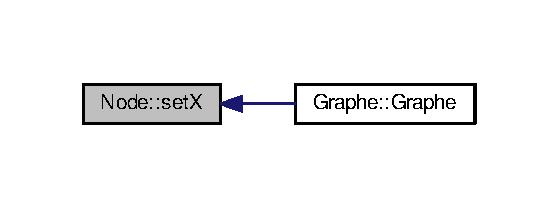
\includegraphics[width=268pt]{class_node_accabc02cdc5144636cab8d5079619d13_icgraph}
\end{center}
\end{figure}


\index{Node@{Node}!set\-Y@{set\-Y}}
\index{set\-Y@{set\-Y}!Node@{Node}}
\subsubsection[{set\-Y}]{\setlength{\rightskip}{0pt plus 5cm}void Node\-::set\-Y (
\begin{DoxyParamCaption}
\item[{int}]{val}
\end{DoxyParamCaption}
)\hspace{0.3cm}{\ttfamily [inline]}}\label{class_node_a475dd9a2117954dbfa44f8cd196d6008}


Setter de l'attribut m\-\_\-\-Y de la classe \doxyref{Node}{p.}{class_node}. 


\begin{DoxyParams}{Paramètres}
{\em val} & \-: valeur de l'attribut a modifier \\
\hline
\end{DoxyParams}


Voici le graphe des appelants de cette fonction \-:
\nopagebreak
\begin{figure}[H]
\begin{center}
\leavevmode
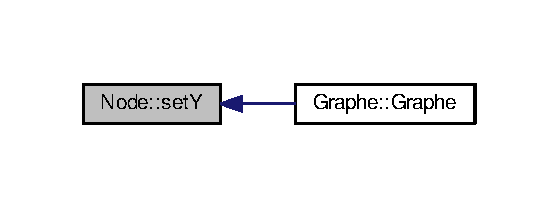
\includegraphics[width=268pt]{class_node_a475dd9a2117954dbfa44f8cd196d6008_icgraph}
\end{center}
\end{figure}




La documentation de cette classe a été générée à partir des fichiers suivants \-:\begin{DoxyCompactItemize}
\item 
code/include/{\bf Node.\-h}\item 
code/src/Node.\-cpp\end{DoxyCompactItemize}

\section{Référence de la classe Pathfinder}
\label{class_pathfinder}\index{Pathfinder@{Pathfinder}}


Classe representant une instance de l'algorithme A$\ast$.  




{\ttfamily \#include $<$Path\-Finder.\-h$>$}

\subsection*{Fonctions membres publiques}
\begin{DoxyCompactItemize}
\item 
{\bf Pathfinder} ()
\begin{DoxyCompactList}\small\item\em Constructeur. \end{DoxyCompactList}\item 
std\-::vector$<$ {\bf Node} $\ast$ $>$ {\bf find\-Path} (std\-::vector$<$ std\-::vector$<$ {\bf Node} $\ast$ $>$ $>$ \&graphe, {\bf Node} $\ast$depart, {\bf Node} $\ast$arrive)
\begin{DoxyCompactList}\small\item\em Application de l'algorithme A$\ast$ sur un objet \doxyref{Graphe}{p.}{class_graphe} dans le but de calculer un chemin du node Depart au node Arrivee. \end{DoxyCompactList}\end{DoxyCompactItemize}
\subsection*{Attributs publics statiques}
\begin{DoxyCompactItemize}
\item 
static const int {\bf N\-O\-D\-E\-\_\-\-D\-I\-S\-T\-A\-N\-C\-E\-\_\-\-V\-A\-L\-U\-E} = 100
\item 
static const int {\bf N\-O\-D\-E\-\_\-\-D\-I\-S\-T\-A\-N\-C\-E\-\_\-\-D\-I\-A\-G\-\_\-\-V\-A\-L\-U\-E} = 140
\end{DoxyCompactItemize}


\subsection{Description détaillée}
Classe representant une instance de l'algorithme A$\ast$. 

\subsection{Documentation des constructeurs et destructeur}
\index{Pathfinder@{Pathfinder}!Pathfinder@{Pathfinder}}
\index{Pathfinder@{Pathfinder}!Pathfinder@{Pathfinder}}
\subsubsection[{Pathfinder}]{\setlength{\rightskip}{0pt plus 5cm}Pathfinder\-::\-Pathfinder (
\begin{DoxyParamCaption}
{}
\end{DoxyParamCaption}
)}\label{class_pathfinder_af562d840858cf2b369fcee51f5069456}


Constructeur. 

Constructeur de la classe \doxyref{Pathfinder}{p.}{class_pathfinder} 

\subsection{Documentation des fonctions membres}
\index{Pathfinder@{Pathfinder}!find\-Path@{find\-Path}}
\index{find\-Path@{find\-Path}!Pathfinder@{Pathfinder}}
\subsubsection[{find\-Path}]{\setlength{\rightskip}{0pt plus 5cm}std\-::vector$<$ {\bf Node} $\ast$ $>$ Pathfinder\-::find\-Path (
\begin{DoxyParamCaption}
\item[{std\-::vector$<$ std\-::vector$<$ {\bf Node} $\ast$ $>$ $>$ \&}]{graphe, }
\item[{{\bf Node} $\ast$}]{depart, }
\item[{{\bf Node} $\ast$}]{arrive}
\end{DoxyParamCaption}
)}\label{class_pathfinder_aee6e72cf2b4a9f86c6aa1139618e2167}


Application de l'algorithme A$\ast$ sur un objet \doxyref{Graphe}{p.}{class_graphe} dans le but de calculer un chemin du node Depart au node Arrivee. 


\begin{DoxyParams}{Paramètres}
{\em graphe} & \-: Objet de type \doxyref{Graphe}{p.}{class_graphe} \\
\hline
{\em depart} & \-: \doxyref{Node}{p.}{class_node} de depart \\
\hline
{\em arrivee} & \-: \doxyref{Node}{p.}{class_node} d'arrivee \\
\hline
\end{DoxyParams}
\begin{DoxyReturn}{Renvoie}
tableau de node representant le chemin du \doxyref{Node}{p.}{class_node} depart au \doxyref{Node}{p.}{class_node} arrivee 
\end{DoxyReturn}


Voici le graphe d'appel pour cette fonction \-:
\nopagebreak
\begin{figure}[H]
\begin{center}
\leavevmode
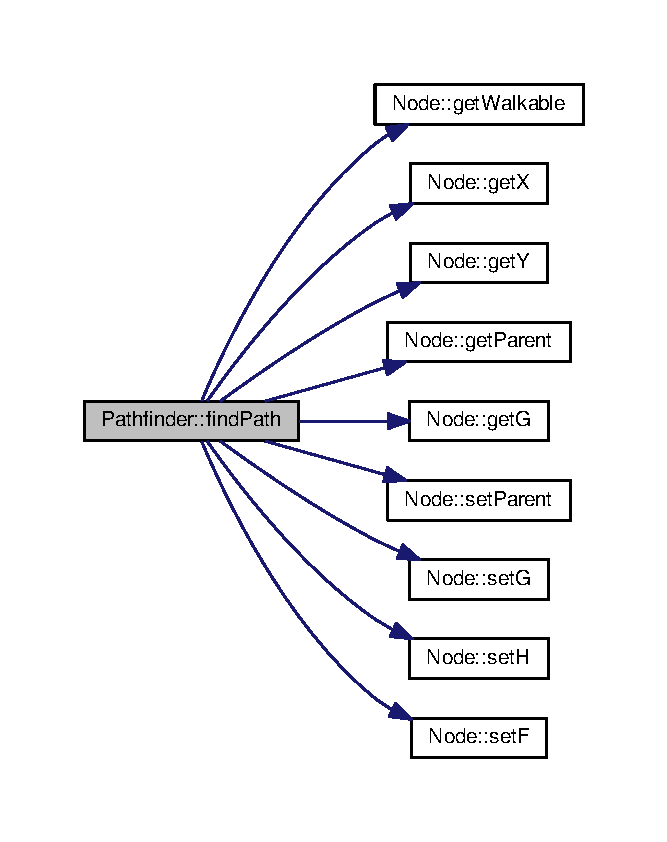
\includegraphics[width=320pt]{class_pathfinder_aee6e72cf2b4a9f86c6aa1139618e2167_cgraph}
\end{center}
\end{figure}




Voici le graphe des appelants de cette fonction \-:
\nopagebreak
\begin{figure}[H]
\begin{center}
\leavevmode
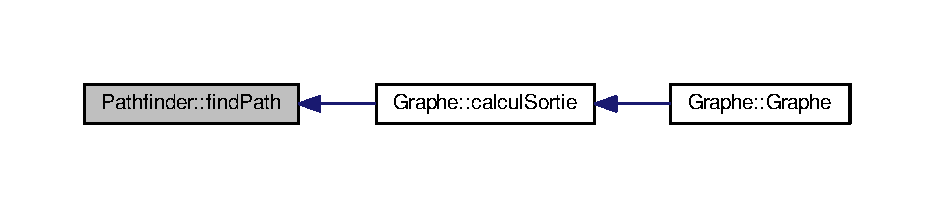
\includegraphics[width=350pt]{class_pathfinder_aee6e72cf2b4a9f86c6aa1139618e2167_icgraph}
\end{center}
\end{figure}




\subsection{Documentation des données membres}
\index{Pathfinder@{Pathfinder}!N\-O\-D\-E\-\_\-\-D\-I\-S\-T\-A\-N\-C\-E\-\_\-\-D\-I\-A\-G\-\_\-\-V\-A\-L\-U\-E@{N\-O\-D\-E\-\_\-\-D\-I\-S\-T\-A\-N\-C\-E\-\_\-\-D\-I\-A\-G\-\_\-\-V\-A\-L\-U\-E}}
\index{N\-O\-D\-E\-\_\-\-D\-I\-S\-T\-A\-N\-C\-E\-\_\-\-D\-I\-A\-G\-\_\-\-V\-A\-L\-U\-E@{N\-O\-D\-E\-\_\-\-D\-I\-S\-T\-A\-N\-C\-E\-\_\-\-D\-I\-A\-G\-\_\-\-V\-A\-L\-U\-E}!Pathfinder@{Pathfinder}}
\subsubsection[{N\-O\-D\-E\-\_\-\-D\-I\-S\-T\-A\-N\-C\-E\-\_\-\-D\-I\-A\-G\-\_\-\-V\-A\-L\-U\-E}]{\setlength{\rightskip}{0pt plus 5cm}const int Pathfinder\-::\-N\-O\-D\-E\-\_\-\-D\-I\-S\-T\-A\-N\-C\-E\-\_\-\-D\-I\-A\-G\-\_\-\-V\-A\-L\-U\-E = 140\hspace{0.3cm}{\ttfamily [static]}}\label{class_pathfinder_a9fabc665d250a89c2f0af4059d77d8b2}
cout d'un deplacement dans les cases voisines D\-I\-A\-G\-O\-N\-A\-L\-E\-S \index{Pathfinder@{Pathfinder}!N\-O\-D\-E\-\_\-\-D\-I\-S\-T\-A\-N\-C\-E\-\_\-\-V\-A\-L\-U\-E@{N\-O\-D\-E\-\_\-\-D\-I\-S\-T\-A\-N\-C\-E\-\_\-\-V\-A\-L\-U\-E}}
\index{N\-O\-D\-E\-\_\-\-D\-I\-S\-T\-A\-N\-C\-E\-\_\-\-V\-A\-L\-U\-E@{N\-O\-D\-E\-\_\-\-D\-I\-S\-T\-A\-N\-C\-E\-\_\-\-V\-A\-L\-U\-E}!Pathfinder@{Pathfinder}}
\subsubsection[{N\-O\-D\-E\-\_\-\-D\-I\-S\-T\-A\-N\-C\-E\-\_\-\-V\-A\-L\-U\-E}]{\setlength{\rightskip}{0pt plus 5cm}const int Pathfinder\-::\-N\-O\-D\-E\-\_\-\-D\-I\-S\-T\-A\-N\-C\-E\-\_\-\-V\-A\-L\-U\-E = 100\hspace{0.3cm}{\ttfamily [static]}}\label{class_pathfinder_a75096e49427cc06e95e82819d949b8e4}
cout d'un deplacement dans les cases voisines H\-A\-U\-T B\-A\-S G\-A\-U\-C\-H\-E ou D\-R\-O\-I\-T\-E 

La documentation de cette classe a été générée à partir des fichiers suivants \-:\begin{DoxyCompactItemize}
\item 
code/include/{\bf Path\-Finder.\-h}\item 
code/src/Path\-Finder.\-cpp\end{DoxyCompactItemize}

\section{Référence de la classe T\-E\-R\-Observer}
\label{class_t_e_r_observer}\index{T\-E\-R\-Observer@{T\-E\-R\-Observer}}


Classe representant un observateur, qui s'occupe de la gestion des agents dans ce processus.  




{\ttfamily \#include $<$T\-E\-R\-Observer.\-h$>$}



Graphe d'héritage de T\-E\-R\-Observer\-:
\nopagebreak
\begin{figure}[H]
\begin{center}
\leavevmode
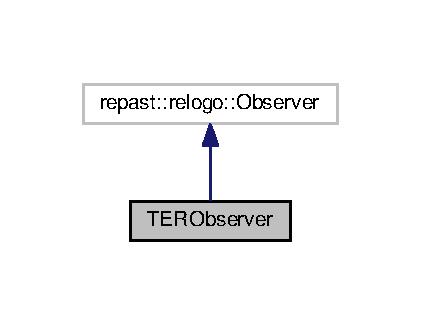
\includegraphics[width=202pt]{class_t_e_r_observer__inherit__graph}
\end{center}
\end{figure}


Graphe de collaboration de T\-E\-R\-Observer\-:
\nopagebreak
\begin{figure}[H]
\begin{center}
\leavevmode
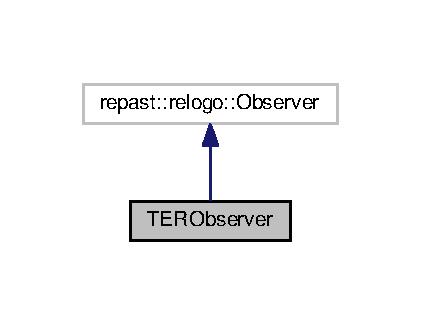
\includegraphics[width=202pt]{class_t_e_r_observer__coll__graph}
\end{center}
\end{figure}
\subsection*{Fonctions membres publiques}
\begin{DoxyCompactItemize}
\item 
{\bf T\-E\-R\-Observer} ()
\begin{DoxyCompactList}\small\item\em Constructeur. \end{DoxyCompactList}\item 
virtual {\bf $\sim$\-T\-E\-R\-Observer} ()
\begin{DoxyCompactList}\small\item\em Destructeur. \end{DoxyCompactList}\item 
void {\bf go} ()\label{class_t_e_r_observer_a87524bb92d6be89b025e4312440f6948}

\begin{DoxyCompactList}\small\item\em Fonction heritee qui est appelee a chaque tick de la simulation. \end{DoxyCompactList}\item 
virtual void {\bf setup} (repast\-::\-Properties \&props)\label{class_t_e_r_observer_a9f04020109fb77d6e704546c7060fff3}

\begin{DoxyCompactList}\small\item\em Fonction heritee qui est appelee a l'initialisation de l'objet Observer. \end{DoxyCompactList}\item 
void {\bf load\-Map\-\_\-a\-\_\-star} (repast\-::\-Properties \&props, std\-::vector$<$ {\bf Coordonnes2\-D} $>$ \&sorties)\label{class_t_e_r_observer_ae8d98b39e6c1f41f2eb78326893106f0}

\begin{DoxyCompactList}\small\item\em Charge a partir du fichier d'initialisation, la matrice map a utiliser pour A$\ast$. \end{DoxyCompactList}\item 
repast\-::relogo\-::\-Relogo\-Agent $\ast$ {\bf create\-Agent} (const {\bf Agent\-Package} \&content)
\begin{DoxyCompactList}\small\item\em Fonction qui cree un agent a partir d'une archive serialisee. \end{DoxyCompactList}\item 
void {\bf provide\-Content} (const repast\-::\-Agent\-Request \&request, std\-::vector$<$ {\bf Agent\-Package} $>$ \&out)
\begin{DoxyCompactList}\small\item\em Fonction qui assigne les valeurs d'un tableau d'archives serialisees a un agent ou un ensemble d'agents. \end{DoxyCompactList}\item 
void {\bf enregister\-Resultats} ()\label{class_t_e_r_observer_a7ef10641e78a9fe2ba24e4fa6fc7e83a}

\begin{DoxyCompactList}\small\item\em Fonction qui enregistre les resultats de la simulation dans un fichier tableur. \end{DoxyCompactList}\item 
void {\bf load\-Map} (repast\-::\-Properties \&props, int process\-\_\-cadran)
\begin{DoxyCompactList}\small\item\em Fonction charge la map a partir du fichier d'initialisation. \end{DoxyCompactList}\item 
void {\bf create\-Agents} (std\-::vector$<$ {\bf Agent\-Package} $>$ \&content, std\-::vector$<$ repast\-::relogo\-::\-Relogo\-Agent $\ast$ $>$ \&out)
\begin{DoxyCompactList}\small\item\em Fonction qui cree des agents, appelee lors d'une synchronisation du buffer de la grille Repast. \end{DoxyCompactList}\item 
void {\bf provide\-Content} (repast\-::relogo\-::\-Relogo\-Agent $\ast$agent, std\-::vector$<$ {\bf Agent\-Package} $>$ \&out)
\begin{DoxyCompactList}\small\item\em Fonction qui fournit aux agents leur contenu, appelee lors d'une synchronisation du buffer de la grille Repast. \end{DoxyCompactList}\item 
void {\bf update\-Agent} ({\bf Agent\-Package} package)
\begin{DoxyCompactList}\small\item\em Fonction qui met à jour des agents deja existants. \end{DoxyCompactList}\item 
void {\bf dessiner\-Decor} (int cadran)
\begin{DoxyCompactList}\small\item\em Fonction qui dessine le decor dans la \doxyref{Fenetre}{p.}{class_fenetre} S\-D\-L. \end{DoxyCompactList}\item 
{\bf Coordonnes2\-D} {\bf Rcor2\-G\-L\-Cor} (int X, int Y, int cadran)
\begin{DoxyCompactList}\small\item\em Fonction qui convertie des cordonnees du monde Repast vers des coordonnes en pixel dans la \doxyref{Fenetre}{p.}{class_fenetre} S\-D\-L associee a ce processus. \end{DoxyCompactList}\item 
{\bf Coordonnes2\-D} {\bf Fcor2\-R\-Cor} (int pos\-X, int pos\-Y)
\begin{DoxyCompactList}\small\item\em Fonction qui convertie des cordonnees du Fichier vers des coordonnes du monde Repast. \end{DoxyCompactList}\item 
{\bf Coordonnes2\-D} {\bf Mcor2\-G\-L\-Cor} (int pos\-X, int pos\-Y)
\begin{DoxyCompactList}\small\item\em Fonction qui convertie des cordonnees de la liste de matrices map vers des coordonnes en pixel de la \doxyref{Fenetre}{p.}{class_fenetre} S\-D\-L. \end{DoxyCompactList}\item 
void {\bf synchronize\-Map} ()\label{class_t_e_r_observer_af7e1247020de2e3d4d42a13ff8c6b6c2}

\begin{DoxyCompactList}\small\item\em Fonction qui synchronise la map et la met a jour en fonction de la map Repast. \end{DoxyCompactList}\item 
void {\bf raz\-Map} ()\label{class_t_e_r_observer_a3b78e3ab9fe3a01b465ccd31f1e88f45}

\begin{DoxyCompactList}\small\item\em Fonction qui remet a 0 la map (liste de matrices en memoire) \end{DoxyCompactList}\item 
{\bf Coordonnes2\-D} {\bf map2\-Repast} ({\bf Coordonnes2\-D} c, int cadran)
\begin{DoxyCompactList}\small\item\em Fonction qui convertit les coordonnes de la map vers des coordonnees Repast. \end{DoxyCompactList}\item 
void {\bf print\-Map} ()\label{class_t_e_r_observer_acb9c7049485c5f1067bf7fd9a1300d28}

\begin{DoxyCompactList}\small\item\em Fonction qui affiche dans la console le contenu de la map (utilise pour debugger) \end{DoxyCompactList}\item 
int {\bf get\-Survivants} ()
\begin{DoxyCompactList}\small\item\em Getter de l'attribut m\-\_\-survivants de la Classe \doxyref{T\-E\-R\-Observer}{p.}{class_t_e_r_observer}. \end{DoxyCompactList}\item 
void {\bf set\-Survivant} (int val)
\begin{DoxyCompactList}\small\item\em Setter de l'attribut m\-\_\-survivants de la Classe \doxyref{T\-E\-R\-Observer}{p.}{class_t_e_r_observer}. \end{DoxyCompactList}\item 
repast\-::\-Properties $\ast$ {\bf get\-Props} ()
\begin{DoxyCompactList}\small\item\em Getter de l'attribut proprietes de la Classe \doxyref{T\-E\-R\-Observer}{p.}{class_t_e_r_observer}. \end{DoxyCompactList}\end{DoxyCompactItemize}


\subsection{Description détaillée}
Classe representant un observateur, qui s'occupe de la gestion des agents dans ce processus. 

\subsection{Documentation des constructeurs et destructeur}
\index{T\-E\-R\-Observer@{T\-E\-R\-Observer}!T\-E\-R\-Observer@{T\-E\-R\-Observer}}
\index{T\-E\-R\-Observer@{T\-E\-R\-Observer}!TERObserver@{T\-E\-R\-Observer}}
\subsubsection[{T\-E\-R\-Observer}]{\setlength{\rightskip}{0pt plus 5cm}T\-E\-R\-Observer\-::\-T\-E\-R\-Observer (
\begin{DoxyParamCaption}
{}
\end{DoxyParamCaption}
)\hspace{0.3cm}{\ttfamily [inline]}}\label{class_t_e_r_observer_aa9e1451ecf894d0b47978a251c33a5bb}


Constructeur. 

Constructeur de la classe \doxyref{T\-E\-R\-Observer}{p.}{class_t_e_r_observer} \index{T\-E\-R\-Observer@{T\-E\-R\-Observer}!$\sim$\-T\-E\-R\-Observer@{$\sim$\-T\-E\-R\-Observer}}
\index{$\sim$\-T\-E\-R\-Observer@{$\sim$\-T\-E\-R\-Observer}!TERObserver@{T\-E\-R\-Observer}}
\subsubsection[{$\sim$\-T\-E\-R\-Observer}]{\setlength{\rightskip}{0pt plus 5cm}virtual T\-E\-R\-Observer\-::$\sim$\-T\-E\-R\-Observer (
\begin{DoxyParamCaption}
{}
\end{DoxyParamCaption}
)\hspace{0.3cm}{\ttfamily [inline]}, {\ttfamily [virtual]}}\label{class_t_e_r_observer_a7aab378089e1835d915d675c1b1aee24}


Destructeur. 

Destructeur de la classe \doxyref{Pathfinder}{p.}{class_pathfinder} 

\subsection{Documentation des fonctions membres}
\index{T\-E\-R\-Observer@{T\-E\-R\-Observer}!create\-Agent@{create\-Agent}}
\index{create\-Agent@{create\-Agent}!TERObserver@{T\-E\-R\-Observer}}
\subsubsection[{create\-Agent}]{\setlength{\rightskip}{0pt plus 5cm}Relogo\-Agent $\ast$ T\-E\-R\-Observer\-::create\-Agent (
\begin{DoxyParamCaption}
\item[{const {\bf Agent\-Package} \&}]{content}
\end{DoxyParamCaption}
)}\label{class_t_e_r_observer_a2ebef6d41d08586bd3b54157ea372f99}


Fonction qui cree un agent a partir d'une archive serialisee. 


\begin{DoxyParams}{Paramètres}
{\em content} & \-: archive serialisee de type \doxyref{Agent\-Package}{p.}{struct_agent_package} \\
\hline
\end{DoxyParams}
\begin{DoxyReturn}{Renvoie}
pointeur sur le nouvel Agent cree en memoire 
\end{DoxyReturn}
\index{T\-E\-R\-Observer@{T\-E\-R\-Observer}!create\-Agents@{create\-Agents}}
\index{create\-Agents@{create\-Agents}!TERObserver@{T\-E\-R\-Observer}}
\subsubsection[{create\-Agents}]{\setlength{\rightskip}{0pt plus 5cm}void T\-E\-R\-Observer\-::create\-Agents (
\begin{DoxyParamCaption}
\item[{std\-::vector$<$ {\bf Agent\-Package} $>$ \&}]{content, }
\item[{std\-::vector$<$ repast\-::relogo\-::\-Relogo\-Agent $\ast$ $>$ \&}]{out}
\end{DoxyParamCaption}
)}\label{class_t_e_r_observer_a33b585c06b752057e20af26a2220a23f}


Fonction qui cree des agents, appelee lors d'une synchronisation du buffer de la grille Repast. 


\begin{DoxyParams}{Paramètres}
{\em content} & \-: archive serialisee de type \doxyref{Agent\-Package}{p.}{struct_agent_package} \\
\hline
{\em out} & \-: reference vers un tableau d'agents a mettre a jour \\
\hline
\end{DoxyParams}
\index{T\-E\-R\-Observer@{T\-E\-R\-Observer}!dessiner\-Decor@{dessiner\-Decor}}
\index{dessiner\-Decor@{dessiner\-Decor}!TERObserver@{T\-E\-R\-Observer}}
\subsubsection[{dessiner\-Decor}]{\setlength{\rightskip}{0pt plus 5cm}void T\-E\-R\-Observer\-::dessiner\-Decor (
\begin{DoxyParamCaption}
\item[{int}]{cadran}
\end{DoxyParamCaption}
)}\label{class_t_e_r_observer_a7b97c7e2c7251d65d946c9ced3c54bcf}


Fonction qui dessine le decor dans la \doxyref{Fenetre}{p.}{class_fenetre} S\-D\-L. 


\begin{DoxyParams}{Paramètres}
{\em cadran} & \-: cadran a dessiner dans ce processus \\
\hline
\end{DoxyParams}


Voici le graphe d'appel pour cette fonction \-:
\nopagebreak
\begin{figure}[H]
\begin{center}
\leavevmode
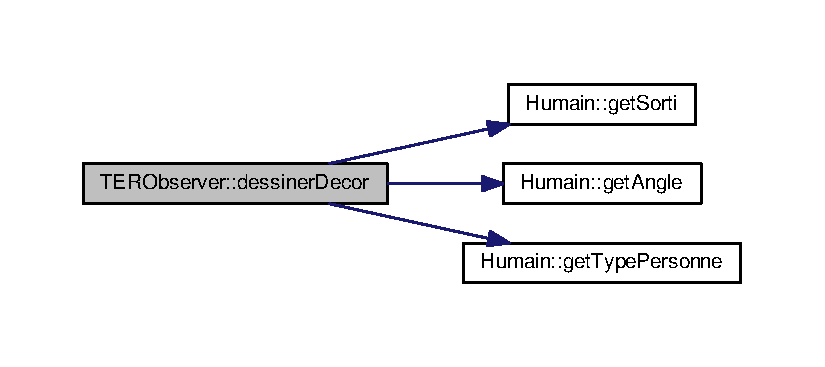
\includegraphics[width=350pt]{class_t_e_r_observer_a7b97c7e2c7251d65d946c9ced3c54bcf_cgraph}
\end{center}
\end{figure}


\index{T\-E\-R\-Observer@{T\-E\-R\-Observer}!Fcor2\-R\-Cor@{Fcor2\-R\-Cor}}
\index{Fcor2\-R\-Cor@{Fcor2\-R\-Cor}!TERObserver@{T\-E\-R\-Observer}}
\subsubsection[{Fcor2\-R\-Cor}]{\setlength{\rightskip}{0pt plus 5cm}{\bf Coordonnes2\-D} T\-E\-R\-Observer\-::\-Fcor2\-R\-Cor (
\begin{DoxyParamCaption}
\item[{int}]{pos\-X, }
\item[{int}]{pos\-Y}
\end{DoxyParamCaption}
)}\label{class_t_e_r_observer_a11cef38b11ca544137fe36e11aba8d5c}


Fonction qui convertie des cordonnees du Fichier vers des coordonnes du monde Repast. 


\begin{DoxyParams}{Paramètres}
{\em X} & \-: coordonne X dans le Fichier \\
\hline
{\em Y} & \-: coordonne Y dans le Fichier \\
\hline
\end{DoxyParams}
\begin{DoxyReturn}{Renvoie}
Un Objet de type \doxyref{Coordonnes2\-D}{p.}{class_coordonnes2_d} contenant les coordonnees converties 
\end{DoxyReturn}
\index{T\-E\-R\-Observer@{T\-E\-R\-Observer}!get\-Props@{get\-Props}}
\index{get\-Props@{get\-Props}!TERObserver@{T\-E\-R\-Observer}}
\subsubsection[{get\-Props}]{\setlength{\rightskip}{0pt plus 5cm}repast\-::\-Properties$\ast$ T\-E\-R\-Observer\-::get\-Props (
\begin{DoxyParamCaption}
{}
\end{DoxyParamCaption}
)\hspace{0.3cm}{\ttfamily [inline]}}\label{class_t_e_r_observer_a8c1de774ac3e1fa31c2233545cae4737}


Getter de l'attribut proprietes de la Classe \doxyref{T\-E\-R\-Observer}{p.}{class_t_e_r_observer}. 

\begin{DoxyReturn}{Renvoie}
l'attribut proprietes de la classe \doxyref{T\-E\-R\-Observer}{p.}{class_t_e_r_observer} 
\end{DoxyReturn}
\index{T\-E\-R\-Observer@{T\-E\-R\-Observer}!get\-Survivants@{get\-Survivants}}
\index{get\-Survivants@{get\-Survivants}!TERObserver@{T\-E\-R\-Observer}}
\subsubsection[{get\-Survivants}]{\setlength{\rightskip}{0pt plus 5cm}int T\-E\-R\-Observer\-::get\-Survivants (
\begin{DoxyParamCaption}
{}
\end{DoxyParamCaption}
)\hspace{0.3cm}{\ttfamily [inline]}}\label{class_t_e_r_observer_a5f19ccb810641760f3623a22cd19fd3c}


Getter de l'attribut m\-\_\-survivants de la Classe \doxyref{T\-E\-R\-Observer}{p.}{class_t_e_r_observer}. 

\begin{DoxyReturn}{Renvoie}
l'attribut m\-\_\-survivants de la classe \doxyref{T\-E\-R\-Observer}{p.}{class_t_e_r_observer} 
\end{DoxyReturn}
\index{T\-E\-R\-Observer@{T\-E\-R\-Observer}!load\-Map@{load\-Map}}
\index{load\-Map@{load\-Map}!TERObserver@{T\-E\-R\-Observer}}
\subsubsection[{load\-Map}]{\setlength{\rightskip}{0pt plus 5cm}void T\-E\-R\-Observer\-::load\-Map (
\begin{DoxyParamCaption}
\item[{repast\-::\-Properties \&}]{props, }
\item[{int}]{process\-\_\-cadran}
\end{DoxyParamCaption}
)}\label{class_t_e_r_observer_ac7815af47779d77ec0ed105af435b186}


Fonction charge la map a partir du fichier d'initialisation. 


\begin{DoxyParams}{Paramètres}
{\em props} & \-: proprietes de la simulation \\
\hline
{\em process\-\_\-cadran} & \-: cadran sur lequel travaille le processus actuel \\
\hline
\end{DoxyParams}
\index{T\-E\-R\-Observer@{T\-E\-R\-Observer}!map2\-Repast@{map2\-Repast}}
\index{map2\-Repast@{map2\-Repast}!TERObserver@{T\-E\-R\-Observer}}
\subsubsection[{map2\-Repast}]{\setlength{\rightskip}{0pt plus 5cm}{\bf Coordonnes2\-D} T\-E\-R\-Observer\-::map2\-Repast (
\begin{DoxyParamCaption}
\item[{{\bf Coordonnes2\-D}}]{c, }
\item[{int}]{cadran}
\end{DoxyParamCaption}
)}\label{class_t_e_r_observer_a51c832c301812eb0cda095e81051d9b0}


Fonction qui convertit les coordonnes de la map vers des coordonnees Repast. 


\begin{DoxyParams}{Paramètres}
{\em c} & \-: Objet de type \doxyref{Coordonnes2\-D}{p.}{class_coordonnes2_d} qui contient les coordonnes de la map à convertir \\
\hline
{\em cadran} & \-: cadran du processus actuel \\
\hline
\end{DoxyParams}
\begin{DoxyReturn}{Renvoie}
Un Objet de type \doxyref{Coordonnes2\-D}{p.}{class_coordonnes2_d} contenant les coordonnees converties 
\end{DoxyReturn}


Voici le graphe d'appel pour cette fonction \-:
\nopagebreak
\begin{figure}[H]
\begin{center}
\leavevmode
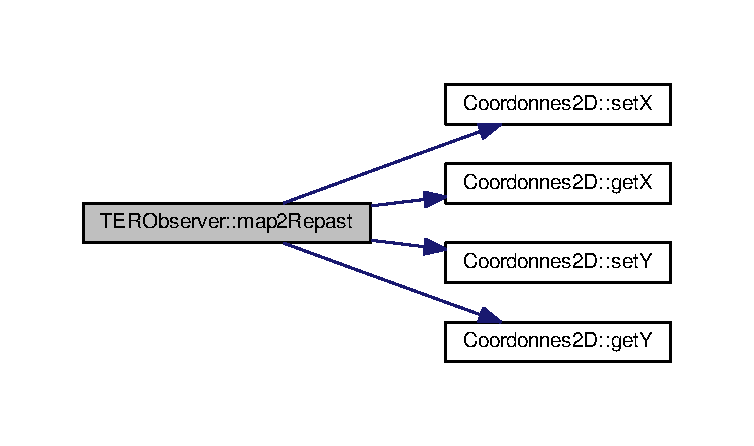
\includegraphics[width=350pt]{class_t_e_r_observer_a51c832c301812eb0cda095e81051d9b0_cgraph}
\end{center}
\end{figure}


\index{T\-E\-R\-Observer@{T\-E\-R\-Observer}!Mcor2\-G\-L\-Cor@{Mcor2\-G\-L\-Cor}}
\index{Mcor2\-G\-L\-Cor@{Mcor2\-G\-L\-Cor}!TERObserver@{T\-E\-R\-Observer}}
\subsubsection[{Mcor2\-G\-L\-Cor}]{\setlength{\rightskip}{0pt plus 5cm}{\bf Coordonnes2\-D} T\-E\-R\-Observer\-::\-Mcor2\-G\-L\-Cor (
\begin{DoxyParamCaption}
\item[{int}]{pos\-X, }
\item[{int}]{pos\-Y}
\end{DoxyParamCaption}
)}\label{class_t_e_r_observer_a5287272e19f0556244cd96a008780d6c}


Fonction qui convertie des cordonnees de la liste de matrices map vers des coordonnes en pixel de la \doxyref{Fenetre}{p.}{class_fenetre} S\-D\-L. 


\begin{DoxyParams}{Paramètres}
{\em X} & \-: coordonne X dans la map \\
\hline
{\em Y} & \-: coordonne Y dans la map \\
\hline
\end{DoxyParams}
\begin{DoxyReturn}{Renvoie}
Un Objet de type \doxyref{Coordonnes2\-D}{p.}{class_coordonnes2_d} contenant les coordonnees converties 
\end{DoxyReturn}
\index{T\-E\-R\-Observer@{T\-E\-R\-Observer}!provide\-Content@{provide\-Content}}
\index{provide\-Content@{provide\-Content}!TERObserver@{T\-E\-R\-Observer}}
\subsubsection[{provide\-Content}]{\setlength{\rightskip}{0pt plus 5cm}void T\-E\-R\-Observer\-::provide\-Content (
\begin{DoxyParamCaption}
\item[{const repast\-::\-Agent\-Request \&}]{request, }
\item[{std\-::vector$<$ {\bf Agent\-Package} $>$ \&}]{out}
\end{DoxyParamCaption}
)}\label{class_t_e_r_observer_ab036cbce36d1f1bd432785277becb041}


Fonction qui assigne les valeurs d'un tableau d'archives serialisees a un agent ou un ensemble d'agents. 


\begin{DoxyParams}{Paramètres}
{\em out} & \-: tableau d'archives serialisees de type \doxyref{Agent\-Package}{p.}{struct_agent_package} \\
\hline
{\em request} & \-: Une requete Repast sur un ou plusieurs agents \\
\hline
\end{DoxyParams}
\begin{DoxyReturn}{Renvoie}
pointeur sur le nouvel Agent cree en memoire 
\end{DoxyReturn}


Voici le graphe d'appel pour cette fonction \-:
\nopagebreak
\begin{figure}[H]
\begin{center}
\leavevmode
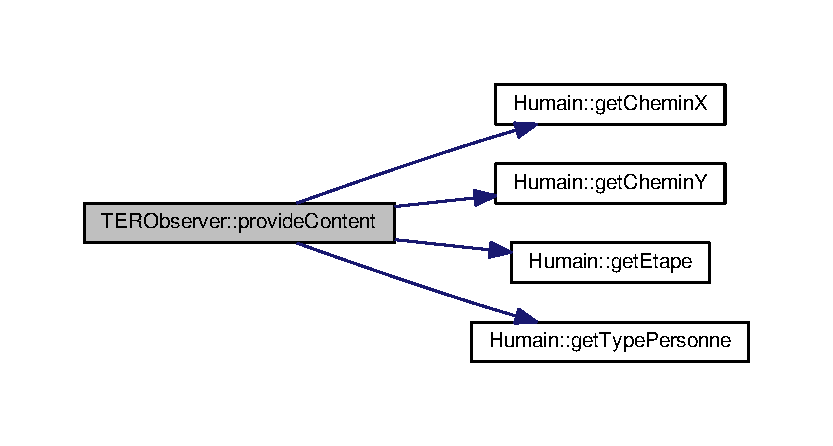
\includegraphics[width=350pt]{class_t_e_r_observer_ab036cbce36d1f1bd432785277becb041_cgraph}
\end{center}
\end{figure}


\index{T\-E\-R\-Observer@{T\-E\-R\-Observer}!provide\-Content@{provide\-Content}}
\index{provide\-Content@{provide\-Content}!TERObserver@{T\-E\-R\-Observer}}
\subsubsection[{provide\-Content}]{\setlength{\rightskip}{0pt plus 5cm}void T\-E\-R\-Observer\-::provide\-Content (
\begin{DoxyParamCaption}
\item[{repast\-::relogo\-::\-Relogo\-Agent $\ast$}]{agent, }
\item[{std\-::vector$<$ {\bf Agent\-Package} $>$ \&}]{out}
\end{DoxyParamCaption}
)}\label{class_t_e_r_observer_a559eb83afbbffd8b6b1d92690e6734ba}


Fonction qui fournit aux agents leur contenu, appelee lors d'une synchronisation du buffer de la grille Repast. 


\begin{DoxyParams}{Paramètres}
{\em agent} & \-: Agent à mettre a jour. \\
\hline
{\em out} & \-: Tableau d'archives serialisees de type \doxyref{Agent\-Package}{p.}{struct_agent_package} \\
\hline
\end{DoxyParams}
\index{T\-E\-R\-Observer@{T\-E\-R\-Observer}!Rcor2\-G\-L\-Cor@{Rcor2\-G\-L\-Cor}}
\index{Rcor2\-G\-L\-Cor@{Rcor2\-G\-L\-Cor}!TERObserver@{T\-E\-R\-Observer}}
\subsubsection[{Rcor2\-G\-L\-Cor}]{\setlength{\rightskip}{0pt plus 5cm}{\bf Coordonnes2\-D} T\-E\-R\-Observer\-::\-Rcor2\-G\-L\-Cor (
\begin{DoxyParamCaption}
\item[{int}]{X, }
\item[{int}]{Y, }
\item[{int}]{cadran}
\end{DoxyParamCaption}
)}\label{class_t_e_r_observer_a6d43b1ce4f72ffe2dafaf6bf831cdec9}


Fonction qui convertie des cordonnees du monde Repast vers des coordonnes en pixel dans la \doxyref{Fenetre}{p.}{class_fenetre} S\-D\-L associee a ce processus. 


\begin{DoxyParams}{Paramètres}
{\em X} & \-: coordonne X dans le monde Repast a convertir \\
\hline
{\em Y} & \-: coordonne Y dans le monde Repast a convertir \\
\hline
{\em cadran} & \-: cadran dans lequel on se trouve \\
\hline
\end{DoxyParams}
\begin{DoxyReturn}{Renvoie}
Un Objet de type \doxyref{Coordonnes2\-D}{p.}{class_coordonnes2_d} contenant les coordonnees converties 
\end{DoxyReturn}
\index{T\-E\-R\-Observer@{T\-E\-R\-Observer}!set\-Survivant@{set\-Survivant}}
\index{set\-Survivant@{set\-Survivant}!TERObserver@{T\-E\-R\-Observer}}
\subsubsection[{set\-Survivant}]{\setlength{\rightskip}{0pt plus 5cm}void T\-E\-R\-Observer\-::set\-Survivant (
\begin{DoxyParamCaption}
\item[{int}]{val}
\end{DoxyParamCaption}
)\hspace{0.3cm}{\ttfamily [inline]}}\label{class_t_e_r_observer_a243d9013eb73de81537e6416561864a4}


Setter de l'attribut m\-\_\-survivants de la Classe \doxyref{T\-E\-R\-Observer}{p.}{class_t_e_r_observer}. 


\begin{DoxyParams}{Paramètres}
{\em val} & \-: l'attribut a affecter a m\-\_\-survivants de la classe \doxyref{T\-E\-R\-Observer}{p.}{class_t_e_r_observer} \\
\hline
\end{DoxyParams}
\index{T\-E\-R\-Observer@{T\-E\-R\-Observer}!update\-Agent@{update\-Agent}}
\index{update\-Agent@{update\-Agent}!TERObserver@{T\-E\-R\-Observer}}
\subsubsection[{update\-Agent}]{\setlength{\rightskip}{0pt plus 5cm}void T\-E\-R\-Observer\-::update\-Agent (
\begin{DoxyParamCaption}
\item[{{\bf Agent\-Package}}]{package}
\end{DoxyParamCaption}
)}\label{class_t_e_r_observer_ab1fe1d3f67f16d7bded15408348bc4b5}


Fonction qui met à jour des agents deja existants. 


\begin{DoxyParams}{Paramètres}
{\em package} & \-: archive serialisee de type \doxyref{Agent\-Package}{p.}{struct_agent_package} \\
\hline
\end{DoxyParams}


Voici le graphe d'appel pour cette fonction \-:
\nopagebreak
\begin{figure}[H]
\begin{center}
\leavevmode
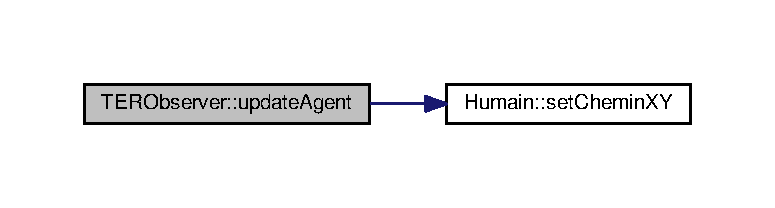
\includegraphics[width=350pt]{class_t_e_r_observer_ab1fe1d3f67f16d7bded15408348bc4b5_cgraph}
\end{center}
\end{figure}




La documentation de cette classe a été générée à partir des fichiers suivants \-:\begin{DoxyCompactItemize}
\item 
code/include/{\bf T\-E\-R\-Observer.\-h}\item 
code/src/T\-E\-R\-Observer.\-cpp\end{DoxyCompactItemize}

\chapter{Documentation des fichiers}
\section{Référence du fichier code/include/\-Agent\-Package.h}
\label{_agent_package_8h}\index{code/include/\-Agent\-Package.\-h@{code/include/\-Agent\-Package.\-h}}


Classe representant une archive serialisee.  


{\ttfamily \#include \char`\"{}repast\-\_\-hpc/\-Agent\-Id.\-h\char`\"{}}\\*
{\ttfamily \#include \char`\"{}boost/serialization/vector.\-hpp\char`\"{}}\\*
Graphe des dépendances par inclusion de Agent\-Package.\-h\-:
\nopagebreak
\begin{figure}[H]
\begin{center}
\leavevmode
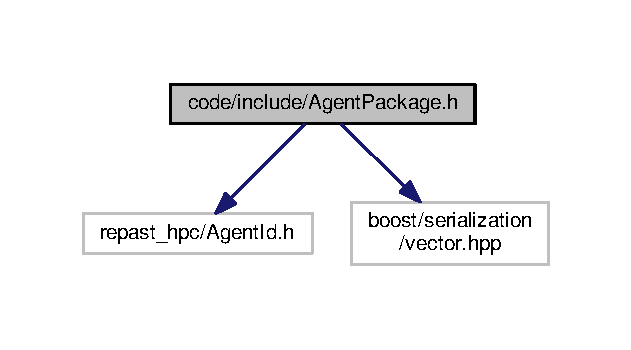
\includegraphics[width=303pt]{_agent_package_8h__incl}
\end{center}
\end{figure}
Ce graphe montre quels fichiers incluent directement ou indirectement ce fichier \-:
\nopagebreak
\begin{figure}[H]
\begin{center}
\leavevmode
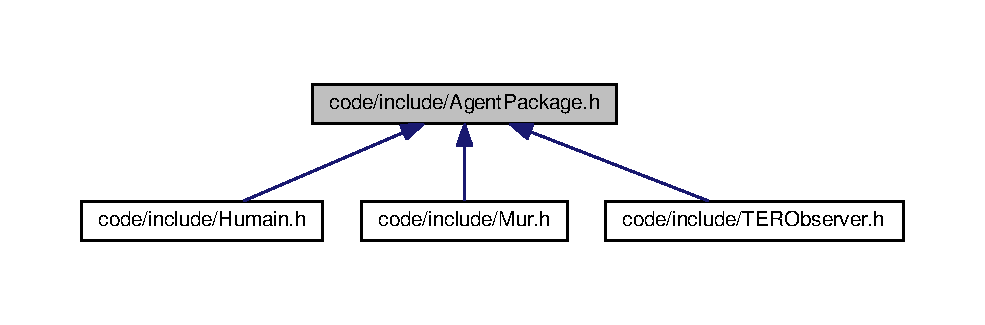
\includegraphics[width=350pt]{_agent_package_8h__dep__incl}
\end{center}
\end{figure}
\subsection*{Classes}
\begin{DoxyCompactItemize}
\item 
struct {\bf Agent\-Package}
\begin{DoxyCompactList}\small\item\em Objet servant d'archive pour le transfert d'attribut des agents d'un processus à un autre. \end{DoxyCompactList}\end{DoxyCompactItemize}


\subsection{Description détaillée}
Classe representant une archive serialisee. \begin{DoxyAuthor}{Auteur}
H\-R\-U\-S\-T\-I\-C E\-M\-I\-R 
\end{DoxyAuthor}
\begin{DoxyVersion}{Version}
0.\-1 
\end{DoxyVersion}

\section{Référence du fichier code/include/coordonnes2d.h}
\label{coordonnes2d_8h}\index{code/include/coordonnes2d.\-h@{code/include/coordonnes2d.\-h}}


Classe representant une position(coordonnees) d'un point.  


Ce graphe montre quels fichiers incluent directement ou indirectement ce fichier \-:
\nopagebreak
\begin{figure}[H]
\begin{center}
\leavevmode
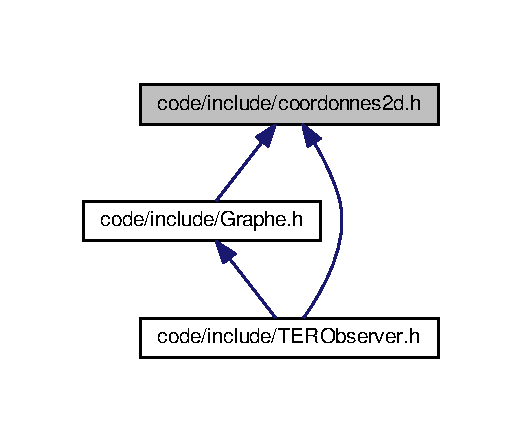
\includegraphics[width=250pt]{coordonnes2d_8h__dep__incl}
\end{center}
\end{figure}
\subsection*{Classes}
\begin{DoxyCompactItemize}
\item 
class {\bf Coordonnes2\-D}
\begin{DoxyCompactList}\small\item\em Classe representant une position(coordonnees) d'un point. \end{DoxyCompactList}\end{DoxyCompactItemize}


\subsection{Description détaillée}
Classe representant une position(coordonnees) d'un point. \begin{DoxyAuthor}{Auteur}
H\-R\-U\-S\-T\-I\-C E\-M\-I\-R 
\end{DoxyAuthor}
\begin{DoxyVersion}{Version}
0.\-1 
\end{DoxyVersion}

\section{Référence du fichier code/include/couleur.h}
\label{couleur_8h}\index{code/include/couleur.\-h@{code/include/couleur.\-h}}


Classe representant une \doxyref{Couleur}{p.}{class_couleur}.  


{\ttfamily \#include $<$S\-D\-L2/\-S\-D\-L.\-h$>$}\\*
Graphe des dépendances par inclusion de couleur.\-h\-:
\nopagebreak
\begin{figure}[H]
\begin{center}
\leavevmode
\includegraphics[width=194pt]{couleur_8h__incl}
\end{center}
\end{figure}
\subsection*{Classes}
\begin{DoxyCompactItemize}
\item 
class {\bf Couleur}
\begin{DoxyCompactList}\small\item\em Classe representant une \doxyref{Couleur}{p.}{class_couleur}. \end{DoxyCompactList}\end{DoxyCompactItemize}


\subsection{Description détaillée}
Classe representant une \doxyref{Couleur}{p.}{class_couleur}. \begin{DoxyAuthor}{Auteur}
H\-R\-U\-S\-T\-I\-C E\-M\-I\-R 
\end{DoxyAuthor}
\begin{DoxyVersion}{Version}
0.\-1 
\end{DoxyVersion}

\section{Référence du fichier code/include/fenetre.h}
\label{fenetre_8h}\index{code/include/fenetre.\-h@{code/include/fenetre.\-h}}


Classe representant une fenetre S\-D\-L.  


{\ttfamily \#include $<$string$>$}\\*
{\ttfamily \#include $<$S\-D\-L2/\-S\-D\-L.\-h$>$}\\*
Graphe des dépendances par inclusion de fenetre.\-h\-:
\nopagebreak
\begin{figure}[H]
\begin{center}
\leavevmode
\includegraphics[width=211pt]{fenetre_8h__incl}
\end{center}
\end{figure}
Ce graphe montre quels fichiers incluent directement ou indirectement ce fichier \-:
\nopagebreak
\begin{figure}[H]
\begin{center}
\leavevmode
\includegraphics[width=350pt]{fenetre_8h__dep__incl}
\end{center}
\end{figure}
\subsection*{Classes}
\begin{DoxyCompactItemize}
\item 
class {\bf Fenetre}
\begin{DoxyCompactList}\small\item\em Classe representant une \doxyref{Fenetre}{p.}{class_fenetre} S\-D\-L. \end{DoxyCompactList}\end{DoxyCompactItemize}


\subsection{Description détaillée}
Classe representant une fenetre S\-D\-L. \begin{DoxyAuthor}{Auteur}
H\-R\-U\-S\-T\-I\-C E\-M\-I\-R 
\end{DoxyAuthor}
\begin{DoxyVersion}{Version}
0.\-1 
\end{DoxyVersion}

\section{Référence du fichier code/include/\-Graphe.h}
\label{_graphe_8h}\index{code/include/\-Graphe.\-h@{code/include/\-Graphe.\-h}}


Classe representant le monde Repast en memoire afin d'appliquer l'algorithme A$\ast$.  


{\ttfamily \#include $<$vector$>$}\\*
{\ttfamily \#include \char`\"{}Node.\-h\char`\"{}}\\*
{\ttfamily \#include \char`\"{}coordonnes2d.\-h\char`\"{}}\\*
{\ttfamily \#include \char`\"{}Path\-Finder.\-h\char`\"{}}\\*
Graphe des dépendances par inclusion de Graphe.\-h\-:
\nopagebreak
\begin{figure}[H]
\begin{center}
\leavevmode
\includegraphics[width=286pt]{_graphe_8h__incl}
\end{center}
\end{figure}
Ce graphe montre quels fichiers incluent directement ou indirectement ce fichier \-:
\nopagebreak
\begin{figure}[H]
\begin{center}
\leavevmode
\includegraphics[width=222pt]{_graphe_8h__dep__incl}
\end{center}
\end{figure}
\subsection*{Classes}
\begin{DoxyCompactItemize}
\item 
class {\bf Graphe}
\begin{DoxyCompactList}\small\item\em Classe representant le monde Repast en memoire. \end{DoxyCompactList}\end{DoxyCompactItemize}


\subsection{Description détaillée}
Classe representant le monde Repast en memoire afin d'appliquer l'algorithme A$\ast$. \begin{DoxyAuthor}{Auteur}
H\-R\-U\-S\-T\-I\-C E\-M\-I\-R 
\end{DoxyAuthor}
\begin{DoxyVersion}{Version}
0.\-1 
\end{DoxyVersion}

\section{Référence du fichier code/include/\-Humain.h}
\label{_humain_8h}\index{code/include/\-Humain.\-h@{code/include/\-Humain.\-h}}


Classe representant un agent \doxyref{Humain}{p.}{class_humain}.  


{\ttfamily \#include \char`\"{}relogo/\-Turtle.\-h\char`\"{}}\\*
{\ttfamily \#include \char`\"{}repast\-\_\-hpc/\-Repast\-Process.\-h\char`\"{}}\\*
{\ttfamily \#include \char`\"{}Agent\-Package.\-h\char`\"{}}\\*
{\ttfamily \#include \char`\"{}fenetre.\-h\char`\"{}}\\*
{\ttfamily \#include \char`\"{}repast\-\_\-hpc/\-Properties.\-h\char`\"{}}\\*
Graphe des dépendances par inclusion de Humain.\-h\-:
\nopagebreak
\begin{figure}[H]
\begin{center}
\leavevmode
\includegraphics[width=350pt]{_humain_8h__incl}
\end{center}
\end{figure}
\subsection*{Classes}
\begin{DoxyCompactItemize}
\item 
class {\bf Humain}
\begin{DoxyCompactList}\small\item\em classe representant un agent humain \end{DoxyCompactList}\end{DoxyCompactItemize}
\subsection*{Macros}
\begin{DoxyCompactItemize}
\item 
\#define {\bfseries T\-A\-U\-X\-\_\-\-P\-E\-R\-S\-O\-N\-N\-E\-S\-\_\-\-A\-G\-E\-E\-S}~5\label{_humain_8h_a544c9c868e9230902e884081c3eea8b6}

\item 
\#define {\bfseries T\-A\-U\-X\-\_\-\-P\-E\-R\-S\-O\-N\-N\-E\-S\-\_\-\-J\-E\-U\-N\-E\-S}~70\label{_humain_8h_a3b4ba41fddcbfd6bc6da3b5d1c470c42}

\item 
\#define {\bfseries T\-A\-U\-X\-\_\-\-P\-E\-R\-S\-O\-N\-N\-E\-S\-\_\-\-A\-D\-U\-L\-T\-E\-S}~20\label{_humain_8h_a3ea4c0823abadc32c7467338f7e10248}

\item 
\#define {\bfseries T\-A\-U\-X\-\_\-\-P\-E\-R\-S\-O\-N\-N\-E\-S\-\_\-\-M\-A\-L\-A\-D\-E\-S}~5\label{_humain_8h_a265aa56b275b328d6800864e06e66886}

\item 
\#define {\bfseries P\-E\-R\-S\-O\-N\-N\-E\-\_\-\-A\-D\-U\-L\-T\-E}~0\label{_humain_8h_add48096cd6292d7b25721b4af3d6e8a3}

\item 
\#define {\bfseries P\-E\-R\-S\-O\-N\-N\-E\-\_\-\-J\-E\-U\-N\-E}~1\label{_humain_8h_a27252b6299c4d107eb363a491e4af6d9}

\item 
\#define {\bfseries P\-E\-R\-S\-O\-N\-N\-E\-\_\-\-A\-G\-E\-E}~2\label{_humain_8h_a32f0282425458046b621418082a6cb9c}

\item 
\#define {\bfseries P\-E\-R\-S\-O\-N\-N\-E\-\_\-\-M\-A\-L\-A\-D\-E}~3\label{_humain_8h_ac639f3633287df1dadde75c60b28eb1e}

\end{DoxyCompactItemize}


\subsection{Description détaillée}
Classe representant un agent \doxyref{Humain}{p.}{class_humain}. \begin{DoxyAuthor}{Auteur}
H\-R\-U\-S\-T\-I\-C E\-M\-I\-R 
\end{DoxyAuthor}
\begin{DoxyVersion}{Version}
0.\-1 
\end{DoxyVersion}

\section{Référence du fichier code/include/\-Mur.h}
\label{_mur_8h}\index{code/include/\-Mur.\-h@{code/include/\-Mur.\-h}}


Classe representant un \doxyref{Mur}{p.}{class_mur}.  


{\ttfamily \#include \char`\"{}relogo/\-Turtle.\-h\char`\"{}}\\*
{\ttfamily \#include \char`\"{}repast\-\_\-hpc/\-Repast\-Process.\-h\char`\"{}}\\*
{\ttfamily \#include \char`\"{}Agent\-Package.\-h\char`\"{}}\\*
{\ttfamily \#include \char`\"{}fenetre.\-h\char`\"{}}\\*
{\ttfamily \#include \char`\"{}repast\-\_\-hpc/\-Properties.\-h\char`\"{}}\\*
Graphe des dépendances par inclusion de Mur.\-h\-:
\nopagebreak
\begin{figure}[H]
\begin{center}
\leavevmode
\includegraphics[width=350pt]{_mur_8h__incl}
\end{center}
\end{figure}
\subsection*{Classes}
\begin{DoxyCompactItemize}
\item 
class {\bf Mur}
\begin{DoxyCompactList}\small\item\em Classe representant un \doxyref{Mur}{p.}{class_mur}. \end{DoxyCompactList}\end{DoxyCompactItemize}


\subsection{Description détaillée}
Classe representant un \doxyref{Mur}{p.}{class_mur}. \begin{DoxyAuthor}{Auteur}
H\-R\-U\-S\-T\-I\-C E\-M\-I\-R 
\end{DoxyAuthor}
\begin{DoxyVersion}{Version}
0.\-1 
\end{DoxyVersion}

\section{Référence du fichier code/include/\-Node.h}
\label{_node_8h}\index{code/include/\-Node.\-h@{code/include/\-Node.\-h}}


Classe representant un \doxyref{Node}{p.}{class_node}.  


Ce graphe montre quels fichiers incluent directement ou indirectement ce fichier \-:
\nopagebreak
\begin{figure}[H]
\begin{center}
\leavevmode
\includegraphics[width=263pt]{_node_8h__dep__incl}
\end{center}
\end{figure}
\subsection*{Classes}
\begin{DoxyCompactItemize}
\item 
class {\bf Node}
\begin{DoxyCompactList}\small\item\em Classe representant un \doxyref{Node}{p.}{class_node} Un \doxyref{Node}{p.}{class_node} est une \char`\"{}case\char`\"{} de la matrice representant le monde Repast, chaque node contient les heuristiques,g,h et f, une position X et Y , un \doxyref{Node}{p.}{class_node} Parent, et un boolean indiquant si le node est un mur ou pas. \end{DoxyCompactList}\end{DoxyCompactItemize}


\subsection{Description détaillée}
Classe representant un \doxyref{Node}{p.}{class_node}. \begin{DoxyAuthor}{Auteur}
H\-R\-U\-S\-T\-I\-C E\-M\-I\-R 
\end{DoxyAuthor}
\begin{DoxyVersion}{Version}
0.\-1 
\end{DoxyVersion}

\section{Référence du fichier code/include/\-Path\-Finder.h}
\label{_path_finder_8h}\index{code/include/\-Path\-Finder.\-h@{code/include/\-Path\-Finder.\-h}}


Classe representant une instance de l'algorithme A$\ast$.  


{\ttfamily \#include \char`\"{}Node.\-h\char`\"{}}\\*
{\ttfamily \#include $<$vector$>$}\\*
Graphe des dépendances par inclusion de Path\-Finder.\-h\-:
\nopagebreak
\begin{figure}[H]
\begin{center}
\leavevmode
\includegraphics[width=210pt]{_path_finder_8h__incl}
\end{center}
\end{figure}
Ce graphe montre quels fichiers incluent directement ou indirectement ce fichier \-:
\nopagebreak
\begin{figure}[H]
\begin{center}
\leavevmode
\includegraphics[width=222pt]{_path_finder_8h__dep__incl}
\end{center}
\end{figure}
\subsection*{Classes}
\begin{DoxyCompactItemize}
\item 
class {\bf Pathfinder}
\begin{DoxyCompactList}\small\item\em Classe representant une instance de l'algorithme A$\ast$. \end{DoxyCompactList}\end{DoxyCompactItemize}


\subsection{Description détaillée}
Classe representant une instance de l'algorithme A$\ast$. \begin{DoxyAuthor}{Auteur}
H\-R\-U\-S\-T\-I\-C E\-M\-I\-R 
\end{DoxyAuthor}
\begin{DoxyVersion}{Version}
0.\-1 
\end{DoxyVersion}

\section{Référence du fichier code/include/\-T\-E\-R\-Observer.h}
\label{_t_e_r_observer_8h}\index{code/include/\-T\-E\-R\-Observer.\-h@{code/include/\-T\-E\-R\-Observer.\-h}}


Classe representant un \doxyref{T\-E\-R\-Observer}{p.}{class_t_e_r_observer}.  


{\ttfamily \#include $<$boost/mpi.\-hpp$>$}\\*
{\ttfamily \#include \char`\"{}relogo/\-Observer.\-h\char`\"{}}\\*
{\ttfamily \#include \char`\"{}repast\-\_\-hpc/\-Agent\-Request.\-h\char`\"{}}\\*
{\ttfamily \#include \char`\"{}repast\-\_\-hpc/\-Properties.\-h\char`\"{}}\\*
{\ttfamily \#include \char`\"{}coordonnes2d.\-h\char`\"{}}\\*
{\ttfamily \#include \char`\"{}Graphe.\-h\char`\"{}}\\*
{\ttfamily \#include $<$list$>$}\\*
{\ttfamily \#include \char`\"{}Agent\-Package.\-h\char`\"{}}\\*
{\ttfamily \#include \char`\"{}fenetre.\-h\char`\"{}}\\*
Graphe des dépendances par inclusion de T\-E\-R\-Observer.\-h\-:
\nopagebreak
\begin{figure}[H]
\begin{center}
\leavevmode
\includegraphics[width=350pt]{_t_e_r_observer_8h__incl}
\end{center}
\end{figure}
\subsection*{Classes}
\begin{DoxyCompactItemize}
\item 
class {\bf T\-E\-R\-Observer}
\begin{DoxyCompactList}\small\item\em Classe representant un observateur, qui s'occupe de la gestion des agents dans ce processus. \end{DoxyCompactList}\end{DoxyCompactItemize}
\subsection*{Macros}
\begin{DoxyCompactItemize}
\item 
\#define {\bfseries N\-B\-\_\-\-P\-R\-O\-C\-E\-S\-S}~4\label{_t_e_r_observer_8h_a42fd4445197ac64796acc0b1deb1a4cd}

\item 
\#define {\bfseries N\-B\-\_\-\-C\-A\-S\-E\-S\-\_\-\-H\-A\-U\-T\-E\-U\-R}~20\label{_t_e_r_observer_8h_a706cc2910571d1667d5d92ce4b92c215}

\item 
\#define {\bfseries N\-B\-\_\-\-C\-A\-S\-E\-S\-\_\-\-L\-A\-R\-G\-E\-U\-R}~20\label{_t_e_r_observer_8h_a05e7c3ac07a9656bf708e6556321e8c1}

\end{DoxyCompactItemize}


\subsection{Description détaillée}
Classe representant un \doxyref{T\-E\-R\-Observer}{p.}{class_t_e_r_observer}. \begin{DoxyAuthor}{Auteur}
H\-R\-U\-S\-T\-I\-C E\-M\-I\-R 
\end{DoxyAuthor}
\begin{DoxyVersion}{Version}
0.\-1 
\end{DoxyVersion}

%--- End generated contents ---

% Index
\newpage
\phantomsection
\addcontentsline{toc}{chapter}{Index}
\printindex

\end{document}
